%%%%%%%%%%%%%%%%%%%%%%%%%%%%%%%%%%%%%%%%%
% Masters/Doctoral Thesis 
% LaTeX Template
% Version 2.5 (27/8/17)
%
% This template was downloaded from:
% http://www.LaTeXTemplates.com
%
% Version 2.x major modifications by:
% Vel (vel@latextemplates.com)
%
% This template is based on a template by:
% Steve Gunn (http://users.ecs.soton.ac.uk/srg/softwaretools/document/templates/)
% Sunil Patel (http://www.sunilpatel.co.uk/thesis-template/)
%
% Template license:
% CC BY-NC-SA 3.0 (http://creativecommons.org/licenses/by-nc-sa/3.0/)
%
%%%%%%%%%%%%%%%%%%%%%%%%%%%%%%%%%%%%%%%%%

%%%%%%%%%%%%%%%%%%%%%%%%%%%%%%%%%%%%%%%%
% PACKAGES AND DOCUMENT CONFIGURATIONS %
%%%%%%%%%%%%%%%%%%%%%%%%%%%%%%%%%%%%%%%%

\documentclass[
11pt, % The default document font size, options: 10pt, 11pt, 12pt
oneside, % Two side (alternating margins) for binding by default, uncomment to switch to one side
english, % ngerman for German
onehalfspacing, % Single line spacing, alternatives: onehalfspacing or doublespacing
%draft, % Uncomment to enable draft mode (no pictures, no links, overfull hboxes indicated)
nolistspacing, % If the document is onehalfspacing or doublespacing, uncomment this to set spacing in lists to single
liststotoc, % Uncomment to add the list of figures/tables/etc to the table of contents
%toctotoc, % Uncomment to add the main table of contents to the table of contents
parskip, % Uncomment to add space between paragraphs
%nohyperref, % Uncomment to not load the hyperref package
headsepline, % Uncomment to get a line under the header
% chapterinoneline, % Uncomment to place the chapter title next to the number on one line
% consistentlayout, % Uncomment to change the layout of the declaration, abstract and acknowledgements pages to match the default layout
]{MastersDoctoralThesis} % The class file specifying the document structure

\usepackage{ifthen} % for conditional statements
    \newboolean{printlayout}
    \setboolean{printlayout}{false} % True for print version

\usepackage{changepage} % for adjustwidth
\usepackage{fontenc} % Output font encoding for international characters
\usepackage{libertine} % Use the Libertine font by default
\usepackage[protrusion=true]{microtype} % Slightly tweak font spacing for aesthetics

\usepackage{adjustbox} % center overlarge elements
\usepackage{algorithm} % for algorithms and pseudo code
\usepackage{algpseudocode} % for algorithms and pseudo code
\usepackage{amssymb} % for symbols
\usepackage[autostyle=true]{csquotes} % Required to generate language-dependent quotes
\usepackage{indentfirst} % indent first line of paragraph, including first in chapter
    \setlength{\parindent}{10pt} % Set paragraph indentation
\usepackage{pdflscape} % landscape pages

\usepackage{float} % strict placement of figures
\usepackage{graphics, subcaption} % Required for including images with lower captions
\usepackage{rotating} % rotate figures
\usepackage{wrapfig} % wrap text around figures

\usepackage{booktabs} % table optimization
\usepackage{colortbl} % color tables
\usepackage{enumitem} % for lists
    \setlist[enumerate]{noitemsep, topsep=0pt}
\usepackage{multirow} % for expanded rows in tables
\usepackage{tabularray} % for tables
\usepackage{xcolor} % custom colors
    \definecolor{hd-red}{RGB}{142, 14, 31} % custom color for the title page
    \definecolor{best}{RGB}{182, 227, 221} % custom color for tables
    \definecolor{worst}{RGB}{240, 222, 176}% custom color for tables
    \definecolor{good}{RGB}{83, 178, 168}% custom color for tables
    \definecolor{bad}{RGB}{209, 159, 89}% custom color for tables

\usepackage{url} % for urls
\usepackage{xurl} % word wrap for links
    \def\UrlFont{\emph} % links are italic

\usepackage{hyperref} % for hyperlinks inside the PDF
\usepackage[nomain,acronyms,automake]{glossaries-extra} % for abbreviations
\usepackage[backend=biber, style=apa, natbib=true, sorting=nyt, isbn=false]{biblatex} % Use the bibtex backend with the APA citation style
    \addbibresource{literature.bib} % The filename of the bibliography
    \renewcommand*{\bibfont}{\small}

% arrows and colors for tables
\newcommand{\upgood}{\color{good}$\uparrow$}
\newcommand{\downgood}{\color{good}$\downarrow$}
\newcommand{\upbad}{\color{bad}$\uparrow$}
\newcommand{\downbad}{\color{bad}$\downarrow$}
\newcommand{\best}{\cellcolor{best}}
\newcommand{\worst}{\cellcolor{worst}}

\newcommand{\comment}[1]{} % enable comment blocks

%%%%%%%%%%%%%%%%%%
% PAPER SETTINGS %
%%%%%%%%%%%%%%%%%%

\geometry{
	paper=a4paper, % Change to letterpaper for US letter
	inner=2.5cm, % Inner margin
	outer=2.5cm, % Outer margin
	bindingoffset=0.0cm, % Binding offset - was 0.5
	top=1.5cm, % Top margin
	bottom=1.5cm, % Bottom margin
	% showframe, % Uncomment to show how the type block is set on the page
}

%%%%%%%%%%%%%%%%%%%%%%
% THESIS INFORMATION %
%%%%%%%%%%%%%%%%%%%%%%

\thesistitle{Enhancing LULC Semantic Segmentation Models by Integrating Spatial Contextual Information from OpenStreetMap Road Networks} % Your thesis title, this is used in the title and abstract, print it elsewhere with \ttitle
\supervisor{apl. Prof. Dr. Sven \textsc{Lautenbach}} % Your supervisor's name, this is used in the title page, print it elsewhere with \supname
\examiner{Dr. Christina \textsc{Ludwig}} % Your examiner's name, this is not currently used anywhere in the template, print it elsewhere with \examname
\degree{Master of Science} % Your degree name, this is used in the title page and abstract, print it elsewhere with \degreename
\author{Nikolaos \textsc{Kolaxidis}} % Your name, this is used in the title page and abstract, print it elsewhere with \authorname
\university{\href{https://www.uni-heidelberg.de/en}{Heidelberg University}} % Your university's name and URL, this is used in the title page and abstract, print it elsewhere with \univname
\department{\href{https://www.geog.uni-heidelberg.de/index_en.html}{Institute of Geography}} % Your department's name and URL, this is used in the title page and abstract, print it elsewhere with \deptname
\group{\href{https://www.geog.uni-heidelberg.de/gis/index_en.html}{GIScience}} % Your research group's name and URL, this is used in the title page, print it elsewhere with \groupname
\faculty{\href{https://www.uni-heidelberg.de/fakultaeten/chemgeo/}{Faculty of Chemistry and Earth Sciences}} % Your faculty's name and URL, this is used in the title page and abstract, print it elsewhere with \facname

\AtBeginDocument{
\hypersetup{pdftitle=\ttitle} % Set the PDF's title to your title
\hypersetup{pdfauthor=\authorname} % Set the PDF's author to your name
% \hypersetup{pdfkeywords=\keywordnames} % Set the PDF's keywords to your keywords
\hypersetup{hidelinks} % hide links
% If you want to have obvious links in the PDF but not the printed text, use:
% \hypersetup{colorlinks=false}.
}

\makeglossaries
% in alphabetical order

% \gls{ai} -> Artificial Intelligence (AI) on first use, then AI on subsequent uses
% \glspl{ai} -> Artificial Intelligences (AIs) on first use, then AIs on subsequent uses
% \glsentrylong{ai} -> Artificial Intelligence
% \glsfmtshort{ai} -> AI

\newabbreviation{ai}{AI}{Artificial Intelligence}
\newabbreviation{ann}{ANN}{Artificial Neural Network}
\newabbreviation{aoi}{AOI}{Area of Interest}
\newabbreviation{ca}{CA}{Class-Wise Accuracy}
\newabbreviation{cle}{CLE}{Cross-Entropy Loss}
\newabbreviation{cnn}{CNN}{Convolutional Neural Network}
\newabbreviation{cpu}{CPU}{Central Processing Unit}
\newabbreviation{cuda}{CUDA}{Compute Unified Device Architecture}
\newabbreviation{cv}{CV}{Computer Vision}
\newabbreviation{dem}{DEM}{Digital Elevation Model}
\newabbreviation{dl}{DL}{Deep Learning}
\newabbreviation{dnn}{DNN}{Deep Neural Network}
\newabbreviation{esa}{ESA}{European Space Agency}
\newabbreviation{fcn}{FCN}{Fully Convolutional Network}
\newabbreviation{ffn}{FFN}{Feed-Forward Network}
\newabbreviation{fn}{FN}{False Negative}
\newabbreviation{fp}{FP}{False Positive}
\newabbreviation{gelu}{GELU}{Gaussian Error Linear Unit}
\newabbreviation{geoai}{GeoAI}{Geospatial Artificial Intelligence}
\newabbreviation{gpu}{GPU}{Graphics Processing Unit}
\newabbreviation{hca}{HCA}{Hierarchical Clustering Analysis}
\newabbreviation{heigit}{HeiGIT}{Heidelberg Institute for Geoinformation Technology}
\newabbreviation{iou}{IoU}{Intersection over Union}
\newabbreviation{lcbb}{LCBB}{Lane-Count-Based Buffer}
\newabbreviation{lulc}{LULC}{Land Use Land Cover}
\newabbreviation{lulcm}{LULC-M}{Land Use Land Cover Mapping}
\newabbreviation{lulcu}{LULC Utility}{Land Use Land Cover Utility}
\newabbreviation{mahdrnk}{MA-HD-RNK}{Mannheim - Heidelberg - Rhein-Neckar-Kreis}
\newabbreviation{mha}{MHA}{Multi-Head (Self-)Attention}
\newabbreviation{mit}{MiT}{Mix Transformer}
\newabbreviation{ml}{ML}{Machine Learning}
\newabbreviation{mlp}{MLP}{Multi-Layer Perceptron}
\newabbreviation{nan}{NaN}{Not a Number}
\newabbreviation{nlp}{NLP}{Natural Language Processing}
\newabbreviation{nn}{NN}{Neural Network}
\newabbreviation{oa}{OA}{Overall Accuracy}
\newabbreviation{ohe}{OHE}{One-Hot Encoding}
\newabbreviation{os}{OS}{Operating System}
\newabbreviation{osm}{OSM}{OpenStreetMap}
\newabbreviation{ppmc}{PPMC}{Pearson's Product Moment Correlation}
\newabbreviation{pvt}{PVT}{Pyramid Vision Transformer}
\newabbreviation{ram}{RAM}{Random Access Memory}
\newabbreviation{relu}{ReLU}{Rectified Linear Unit}
\newabbreviation{resnet}{ResNet}{Residual Network}
\newabbreviation{rf}{RF}{RandomForest}
\newabbreviation{sdg}{SDG}{Sustainable Development Goal}
\newabbreviation{sdpa}{SDPA}{Scaled Dot-Product Attention}
\newabbreviation{setr}{SETR}{Segmentation Transformer}
\newabbreviation{sgd}{SGD}{Stochastic Gradient Descent}
\newabbreviation{tn}{TN}{True Negative}
\newabbreviation{tp}{TP}{True Positive}
\newabbreviation{vit}{ViT}{Vision Transformer}
\newabbreviation{vram}{VRAM}{Video Random Access Memory}
\newabbreviation{wsl}{WSL}{Windows Subsystem Linux} % Load entries from the abbreviations.tex file

%%%%%%%%
% MAIN %
%%%%%%%%

\begin{document}

\frontmatter % Use roman page numbering style (i, ii, iii, iv...) for the pre-content pages

\pagestyle{plain} % Default to the plain heading style until the thesis style is called for the body content

%%%%%%%%%%%%%%
% TITLE PAGE %
%%%%%%%%%%%%%%

\begin{titlepage}
\begin{center}

{\color{hd-red} % Change color as needed
\textsc{\large 
    \univname\\[.4cm] % University name
    \deptname\\ % Department name
    \facname
}}\\[.4cm] % Faculty name
\emph{in cooperation with}\\[.4cm]
{\color{hd-red}
    \textsc{\href{https://heigit.org}{HeiGIT gGmbH}
}}\\[1.2cm]
\textsc{\LARGE Master's Thesis}\\[.8cm] % Thesis type

\HRule \\ % Horizontal line
\vspace{.4cm}
\begin{adjustwidth}{-0.5em}{-0.5em}
    \centering
    {\huge \bfseries \ttitle \par} % Thesis title
\end{adjustwidth}
\vspace{.4cm}
\HRule \\[1.2cm] % Horizontal line
 
\begin{minipage}[t]{.4\textwidth}
\begin{flushleft} \large
\emph{Author:}\\
{\color{hd-red}{\authorname}}
\end{flushleft}
\end{minipage}
\begin{minipage}[t]{.4\textwidth}
\begin{flushright} \large
\emph{First Examiner:} \\
{\color{hd-red}{\supname}} \\
\vspace{.4cm}
\emph{Second Examiner:}\\
{\color{hd-red}
    {\examname} \\
    \emph{associated with \href{https://heigit.org}{HeiGIT gGmbH}}
} \\

\end{flushright}
\end{minipage}\\
 
\vspace{1.6cm}

\large \emph{A thesis submitted in partial fulfillment of\\ the requirements for the degree of}\\[.4cm] % University requirement text
{\color{hd-red}
    \textsc{\degreename
}}\\[.33cm]
\emph{in}\\[.33cm]
{\color{hd-red}
    \textsc{Geography}\\
    Specialization in \textsc{Geoinformatics}
}\\ % Subject
 
\vfill

{\large \today} % Date
 
\end{center}
\end{titlepage}

\ifthenelse{\boolean{printlayout}}{
    \cleardoublepage
    \shipout\null
}{} % insert blank page without increasing page counter for print version

%%%%%%%%%%%%%
% ABSTRACTS %
%%%%%%%%%%%%%

\begin{abstract} % English

Currently, two topics are prevalent in the geographic science world, namely deep learning and climate change. One key research field at the intersection of both fields is \glsentrylong{lulc} (\glsfmtshort{lulc}) mapping, a geographical computer vision task requiring large amounts of remote sensing data and, therefore, suitable deep learning models for segmentation. By utilizing such models, \glsfmtshort{lulc} mapping can be done automatically and efficiently, aiding in environmental monitoring as well as sustainable urban planning and resource management. Deep learning models offer two ways of improvement: enhancing the performance or enhancing the efficiency. In regard to climate change, efficiency becomes more important, as the models should be as sustainable as possible without consuming unnecessary resources. However, the reduction of performance for the sake of efficiency is not a desirable trade-off, especially when the according results are used for further applications. Therefore, this study evaluates a concept of supporting the convergence of models for \glsfmtshort{lulc} mapping in order to reduce the resource consumption while achieving similar performance. Current semantic segmentation models are able to capture a large context area of pixels to classify them effectively with more information available. Hypothetically, for segmentation tasks like \glsfmtshort{lulc} mapping, spatial contextual information has the potential to aid the models in making more informed predictions. As they are an important part of the landscape and are built with the adjacent \glsfmtshort{lulc} areas in mind, roads seem suitable to provide such information. Utilizing the SegFormer architecture inside the \glsfmtshort{lulc} Utility, a cutting-edge semantic segmentation framework for \glsfmtshort{lulc} mapping, this study incorporates features from the OpenStreetMap road network to improve both model performance and resource efficiency. Key research questions focus on identifying relevant road attributes, suitable encoding methods for feature integration, and the impact of these integrations on model performance and resource consumption. The results demonstrate that incorporating road network data, particularly road types and speed limits, considerably enhances the model's performance, while also increasing the resource consumption. However, they also show that with fine-tuning hyperparameters and according optimization techniques, the method has the potential to achieve higher performance while being more efficient, accomplishing the aforementioned goal. The study confirms that the integration of contextual data can be a valuable addition to deep learning models in the field of computer vision, as it offers the potential to enhance both their performance and efficiency.

\end{abstract}

\renewcommand{\abstractname}{Zusammenfassung}  % German
\renewcommand{\byname}{von}
\begin{abstract}

In der geographischen Wissenschaftswelt sind heutzutage zwei Themen nicht wegzudenken: Deep Learning und der Klimawandel. Ein zentrales Forschungsfeld an der Schnittstelle beider Themen ist das Mapping von Landnutzung und Landbedeckung (\glsfmtshort{lulc}), eine geografische Computer Vision-Aufgabe, die vor allem wegen großer Mengen an Fernerkundungsdaten geeignete Deep Learning Modelle für die Segmentierung erfordert. Durch den Einsatz solcher Modelle kann das \glsfmtshort{lulc}-Mapping automatisch und effizient durchgeführt werden, was die Umweltüberwachung sowie die nachhaltige Stadtplanung und Ressourcenverwaltung unterstützt. Deep Learning-Modelle bieten zwei Möglichkeiten zur Verbesserung: die Erhöhung der Performance oder die Verbesserung der Effizienz. In Bezug zum Klimawandel gewinnt die Effizienz immer mehr an Bedeutung, da die Modelle so nachhaltig wie möglich sein sollten, ohne unnötige Ressourcen zu verbrauchen. Allerdings ist eine Reduzierung der Performance zugunsten der Effizienz kein wünschenswerter Kompromiss, insbesondere wenn die Ergebnisse für weitere Anwendungen genutzt werden. Diese Studie evaluiert daher ein Konzept zur Unterstützung der Konvergenz von Modellen für das \glsfmtshort{lulc}-Mapping, um den Ressourcenverbrauch zu reduzieren und gleichzeitig eine ähnliche Performance zu erzielen. Aktuelle Modelle zur semantischen Segmentierung sind in der Lage, einen großen Kontextbereich von Pixeln zu erfassen, um sie mit mehr verfügbaren Informationen effektiver zu klassifizieren. Hypothetisch haben räumliche Kontextinformationen für Segmentierungsaufgaben wie das \glsfmtshort{lulc}-Mapping  das Potenzial, den Modellen zu helfen, fundiertere Vorhersagen zu treffen. Straßen, als wichtiger Teil der Landschaft und in Bezug auf die angrenzenden \glsfmtshort{lulc}-Gebiete gebaut, scheinen geeignet, solche Informationen bereitzustellen. Diese Studie nutzt das SegFormer Modell, eingebettet im \glsfmtshort{lulc} Utility, einem Framework zum \glsfmtshort{lulc}-Mapping, und integriert Features des OpenStreetMap-Straßennetzwerkes, um sowohl die Performance als auch die Ressourceneffizienz des Modells zu verbessern. Die Hauptforschungsfragen konzentrieren sich auf die Identifizierung relevanter Straßeneigenschaften, geeignete Kodierungsmethoden für die Integration von Features und die Auswirkungen der integrierten Kontextinformationen auf die Performance und den Ressourcenverbrauch. Die Ergebnisse zeigen, dass die Einbeziehung von Straßennetzdaten, insbesondere Straßentypen und Geschwindigkeitsbegrenzungen, die Performance des Modells erheblich verbessert, gleichzeitig aber auch den Ressourcenverbrauch erhöht. Sie zeigen allerdings auch, dass mit dem Fine-Tuning der Hyperparameter und entsprechenden Optimierungstechniken die Methode das Potenzial hat, höhere Performance bei höherer Effizienz zu erzielen, und somit das angestrebte Ziel der Kombination von beidem zu erreichen. Die Studie bestätigt, dass die Integration von Kontextdaten eine wertvolle Ergänzung für Deep Learning-Modelle im Bereich des Computer Vision darstellt, da sie das Potenzial bietet, sowohl deren Performance als auch Effizienz zu verbessern.

\end{abstract}

%%%%%%%%%%%%%%%%%%%%
% ACKNOWLEDGEMENTS %
%%%%%%%%%%%%%%%%%%%%

\begin{acknowledgements}

\vspace{.4cm}

% Christina
First and foremost, I would like to express my sincere gratitude to \emph{Dr. Christina Ludwig} for the opportunity of conducting this research, her continuous support, guidance, and insightful discussions that have tremendously enriched this work. Your dedication and knowledge have been invaluable to this study and my academic journey in general.

% Sven
I extend my heartfelt thanks to \emph{apl. Prof. Dr. Sven Lautenbach} for his valuable insights and constructive feedback throughout this research. Your expertise has greatly contributed to the development of this study, including the refinement of the research questions and the overall aim.

% Maciej
Special thanks go to my colleague, \emph{Dr. Maciej Adamiak}, for his assistance, provision of the utilized framework, and inspiration that lay the foundation of this work. Without your limitless inventiveness, creativity, and passion, this thesis would have not been conducted so successfully. Thanks also for enhancing my understanding of the subject matter during the Innovation Weeks and our multiple meetings, this helped me greatly for this thesis.

% Institute of Geography & Heigit
I am grateful to the \emph{Institute of Geography} and the \emph{HeiGIT gGmbH} for providing the resources and environment necessary for the completion of this thesis. 

% Friends and Family
I thank my \emph{family} for continuous support and encouragement throughout my studies. You always had my back and spanned a boundless safety net, enabling me to focus on my studies. Thanks also go to my \emph{friends} for multiple joyful and insightful discussions and experiences.

% Sara
Thanks also to you, \emph{Sara}, without you I would not have left my desk to enjoy the sun in the summer, take relaxing walks, and the office and us would miss a very welcome distraction.

% Bu
Finally, I would like to express my deepest gratitude to \emph{my better half} for unwavering and enduring support, patience, and the best food I could ask for during the long final sprint. Your love and belief in me have been a constant source of motivation and a large driver for my recent development in any aspect.

% Final
Thank you all for giving me the opportunity to grow, learn, and follow my dreams.  Without you, this would not have been possible.

\end{acknowledgements}

\ifthenelse{\boolean{printlayout}}{
    \cleardoublepage
    \shipout\null
}{} % insert blank page without increasing page counter for print version

%%%%%%%%%%%%%%%
% DECLARATION %
%%%%%%%%%%%%%%%

\renewcommand{\authorshipname}{Statutory declaration}
\begin{declaration}

\noindent I, \authorname, declare that this thesis titled, \enquote{\ttitle} and the work presented in it are my own. I confirm that:

\begin{itemize} 
    \item I	have authored this thesis independently.
    \item I have not used other than the declared sources / resources.
    \item I have explicitly marked all material which has been quoted either literally or by content from the used sources.
    \item this paper was not previously presented to another examination board and has not been published.
\end{itemize}

\vspace{1.2cm}

\noindent Dossenheim, \today\\[.4cm]
\rule[.8cm]{15cm}{.5pt} % This prints a line for date and signature
 
\end{declaration}

\ifthenelse{\boolean{printlayout}}{
    \cleardoublepage
    \shipout\null
}{} % insert blank page without increasing page counter for print version

%%%%%%%%%%%%%%%%%%%%%%%%%%%%%%%%%%%%%%%%%%%%%%%%%%%
% LISTS OF CONTENTS/FIGURES/TABLES/ABBREVIATIONS %
%%%%%%%%%%%%%%%%%%%%%%%%%%%%%%%%%%%%%%%%%%%%%%%%%%%

\tableofcontents % Prints the main table of contents
\listoffigures % Prints the list of figures
\listoftables % Prints the list of tables
\printacronyms[nonumberlist, nogroupskip, title=List of Acronyms and Abbreviations] % Prints the list of abbreviations

%%%%%%%%%%%%%%%%%%%%%%%%%%%%%
% THESIS CONTENT - CHAPTERS %
%%%%%%%%%%%%%%%%%%%%%%%%%%%%%

\mainmatter % Begin numeric (1,2,3...) page numbering

\pagestyle{thesis} % Return the page headers back to the "thesis" style

\chapter{Introduction}
\label{sec:intro}

% AI super current with ChatGPT and LLMs
It's everywhere: in the news, in research and science, on the web, in our hands, used in our daily lives as a companion, its usage strongly debated in universities and schools, and its possibilities seemingly endless \autocite{Roumeliotis.Tselikas2023}. \gls{ai} is currently one of the most discussed technological topics thanks to the development of large language models and the emergence of {\nobreak OpenAI's} famous ChatGPT (Generative Pre-Trained Transformer, \autocite{OpenAI2022}) towards the end of 2022, functioning as a chatbot successfully mimicking human conversation \autocite{Abdullah.Madain.ea2022,Alzubaidi.Zhang.ea2021}. Despite its term being coined as far back as 1956 during the Dartmouth Conferences, it is the recent improvements in computational power, networks, and the advent of big data that have truly advanced its growth and application \autocite{Ongsulee2017}. \gls{ai} has already reinvented numerous sectors, from healthcare to finance, by automating tasks, improving decision-making processes, and providing new insights from data \autocite{Alzubaidi.Zhang.ea2021,Bini2018,Ongsulee2017,Roumeliotis.Tselikas2023}.

% ML and Climate Change, SDGs
\gls{ml}, a subfield of \gls{ai} that enables data-driven pattern recognition and sits at the intersection of \gls{ai} and data science, has emerged as a powerful tool for global sustainable development. One of the most critical issues in the 21st century, it aims at fulfilling current requirements of human development without compromising future generations \autocite{UnitedNations2023}. \gls{ml} provides innovative solutions for monitoring and managing natural resources, predicting environmental changes, and driving sustainable practices across various sectors \autocite{Getzner.Charpentier.ea2023,Kar.Choudhary.ea2022,Mehlin.Schacht.ea2023}. Goal 13 \enquote{Climate Action} of the \glspl{sdg}, set by the United Nations to be achieved by 2030, explicitly addresses the need for urgent action to combat climate change and its impacts. Furthermore, goal 11 \enquote{Sustainable Cities and Communities} aims to make cities inclusive, safe, resilient, and sustainable, by addressing comprehensive urban issues such as infrastructure, management, and urban planning, a goal including the advancements in \gls{ai} and, specifically, \gls{ml} and its possibilities for sustainable development \autocite{UnitedNations2023}.

% LULC-M and IPCC
An important geographical research field between \gls{ai} and sustainability is the utilization of \gls{ml} models for \gls{lulcm}, which gains a lot of attention from the need for sustainable development and urban planning \autocite{Zhao.Tu.ea2023}. The Intergovernmental Panel on Climate Change states that \enquote{global greenhouse gas emissions have continued to increase, with unequal historical and ongoing contributions arising from unsustainable energy use, land use and land use change, lifestyles and patterns of consumption and production across regions, between and within countries, and among individuals} \autocite[4]{IPCC2023}. \gls{lulc} is named explicitly as one of the key sectors where more sustainable interaction methods are needed to mitigate climate change, showing its importance in the context of sustainable development.

% What is LULC-M
\gls{lulcm} segments the landscape into patches of different land cover and land use types which gives valuable insights into their distribution and interaction at a given time \autocite{Li.Cai.ea2024}. Its largest potential lies in monitoring human-made and natural landscape changes which enables stakeholders to adapt the anthropogenic land uses in order to act more sustainable in and with the environment \autocite{Moharram.Sundaram2023}. Moreover, it plays a crucial role in diverse sectors such as disaster management, monitoring carbon emissions, and agricultural production, which underlines its broad spectrum of applications \autocite{Alhassan.Henry.ea2020,Rangel.Terven.ea2024,Zhao.Tu.ea2023}.

% Deep Learning for LULC-M
Initially done manually or semi-automated, \gls{lulcm} has been revolutionized by the advent of \gls{ml} and \gls{dl} models, especially image segmentation models, which have significantly improved the accuracy and efficiency of the process \autocite{Zhao.Tu.ea2023}. These models are trained on large datasets of satellite imagery to predict the \gls{lulc} classes of a given area, which can then be used for further analyses like monitoring changes over time and space \autocite{Li.Cai.ea2024}. Especially \gls{dl} models building on the Transformer, serving as the foundation for ChatGPT, have shown great potential in this field due to their ability to capture long-range dependencies and contextual information in images by utilizing attention mechanisms, partially enlarging receptive fields beyond their initial fixed reach \autocite{Alhichri.Alswayed.ea2021,Chen.Yang.ea2016,Xie.Wang.ea2021,Zheng.Lu.ea2021}.

% Environmental impact of ML
However, development and operation of \gls{ml} models require substantial computational resources and energy, which adds negatively to their environmental benefits. This is in particular true for \gls{dl} models as training increasingly complex models for improved accuracy results in greater energy use and carbon emissions \autocite{Desislavov.Martinez-Plumed.ea2023,Mehlin.Schacht.ea2023,Strubell.Ganesh.ea2019}. It is estimated that training a large Transformer model with 213 Million parameters (like a GPT) emits as much carbon dioxide as an average car drive for nearly 400 Kilometers \autocite{Strubell.Ganesh.ea2019,CSS2023}. This shows that the environmental impact of \gls{ml} models is not to be underestimated and that their sustainability has to be addressed alongside improving solely their performance. This ensures the technology's overall viability in the long term, also in respect to the named \glspl{sdg} \autocite{Getzner.Charpentier.ea2023,Thompson.Greenewald.ea2022}.

% Two ways to enhance ML models
So, as the power of \gls{ai} is harnessed for sustainable development, there are two main ways to enhance \gls{ml} and \gls{dl} models: either enhancing the performance by utilizing model improvements or reducing the resource consumption by utilizing sustainable methods for existing models \autocite{Getzner.Charpentier.ea2023,Moharram.Sundaram2023,Zhao.Tu.ea2023}. This is a constant goal in the field of \gls{ml} and \gls{dl} \autocite{Ongsulee2017,Roumeliotis.Tselikas2023}. In order to reduce the consumption of resources, a key strategy involves supporting model convergence with intelligent adaptations along with keeping the accuracies at a similar level, thereby shifting from a \enquote{faster-larger-better} to a \enquote{similar-but-more-efficient} approach \autocite{Lazzaro.Cina.ea2023,Mehlin.Schacht.ea2023,Tao.Meng.ea2022}. But, such a strategy can also enhance the accuracy of the models, as the models can make more informed decisions about the data they are trained on \autocite{Mehlin.Schacht.ea2023}.

% Contextual information
Based on the possibilities brought by the attention mechanisms, larger receptive fields, and the idea of multiple studies, it seems that in the field of \gls{lulcm}, providing spatial contextual information to \gls{dl} models is able to fulfill both roles. \textcite{Zhao.Ning.ea2023} describe the main concept of spatial context using Tobler's First Law of Geography \autocite{Tobler1970}: \enquote{The spatial distribution of geographical things or attributes is interrelated with each other, and it appears with clustering, random, and regular characteristics. The relationship can be described by the spatial context. Hence, spatial context extraction from the surrounding environment of geographic objects can enrich their characteristics and is very useful for predicting their types} \autocite[2]{Zhao.Ning.ea2023}. In their study, they used multiple spatial contexts like intersections, surrounding buildings, and points of interest to predict road types in satellite imagery. Additionally, they used tags from \gls{osm} which added information about traffic behavior and therefore the importance of roads, helping classifying the hierarchically structured road types. \textcite{Xu.Zhou.ea2022,Zong.He.ea2020} also utilized context inclusion, including points of interest and nighttime lights along with other data, to enhance \gls{lulcm}. They and others additionally used road networks from \gls{osm} to divide their \glspl{aoi} into research units and urban segments. \textcite{Forget.Linard.ea2018} went even a step further and assumed a correlation between road network and adjacent urban blocks as well as building types in order to enhance the prediction of built-up areas, an assumption similarly established by \textcite{Ahmadzai2020}. They all showed that including spatial contextual information greatly helps in prediction and can be used to enhance the performance of models, as proposed in its essence as early as in Tobler's First Law of Geography in 1970.

% Aim
This raises the question: if a road network provides additional attributes like road types, can it be utilized to enhance the mapping of all the surrounding \gls{lulc} areas, thus, \gls{lulcm}? This could be a valuable addition to the model, as roads are often built with adjacent \gls{lulc} classes in mind and, therefore, should give hints towards them \autocite{Ahmadzai2020,Levinson.Xie.ea2007,Zeng.Zhao.ea2020}. 

The main task of this study is the evaluation of a contextual inclusion approach which involves the integration of a road network into the feature space of a \gls{lulcm} model through feature engineering. The aim is to enrich the model with valuable spatial contextual information about the adjacent \gls{lulc} classes, given their specific geographical positioning within the landscape and relationship to the road network. Hypothetically, by adding information about the spatial context of \gls{lulc} classes using a road network, the model convergence should be supported and the overall resource consumption reduced alongside an increase of the performance, as the model can make more informed decisions about the \gls{lulc} classes.

% Framework
The \gls{dl} framework selected for assessing this hypothesis is the \gls{lulcu} \autocite{HeiGIT2024a}, a tool developed by the Climate Action focus group of the \gls{heigit} for \gls{lulcm} \autocite{HeiGIT2024}. The \gls{lulcu} utilizes the SegFormer architecture proposed by \textcite{Xie.Wang.ea2021}, a Transformer-based semantic segmentation model originally for RGB images, with adaptations to support multi-spectral satellite bands and a flexible framework to allow for easy integration of additional data sources.

% RQs
The research questions of this study outline the aim of integrating a road network into the feature space of a suitable \gls{dl} model and assessing the impact of integrated spatial contextual information on the model's performance with:\pagebreak

\begin{enumerate}[label={RQ \arabic*:}]
    \item \emph{Which attributes of the \gls{osm} road network can provide the model spatial contextual information regarding \gls{lulc} classes, and what is their relationship to adjacent \gls{lulc} classes derived from \gls{osm}?} 
    \item \emph{What is a suitable encoding method to integrate them into the feature space of the model?}
    \item \emph{How much does the integrated road network and its attributes impact the model's performance and resource consumption?}
\end{enumerate}

% Structure
The further structure of this thesis is organized specifically to address these research questions. First, \gls{lulcm} and the segmentation technique are explained, followed by an introduction to \glspl{dl} for a basic understanding of the training process of neural networks. Later, the background of the SegFormer is explained with a deep dive into attention mechanisms. The methodology outlines the research design used to answer the research questions, including a description of \gls{osm} and utilized datasets, the explorative relationship analysis between select road attributes and \gls{lulc} classes, and the model used as baseline. It further answers RQ 2 by showing four different approaches to integrate the road network into the feature space of the \gls{lulcu}. The results of the experiments are presented and discussed critically in regard to the research questions and similar studies afterwards. The thesis is concluded with an outlook on future research and a summary of the key findings.

\chapter{Theoretical Background}
\label{sec:theory}

This chapter provides the theoretical background for the study. It first gives an introduction to \gls{lulcm} and semantic segmentation. Afterwards, basics of \glspl{nn} and \glspl{dnn} are explained, including training concepts and some milestone model architectures for \gls{cv}. A deeper dive into the attention mechanism and the SegFormer architecture follows, which forms the primary theoretical emphasis of the study. This enables the integration of contextual data into the feature space, which is approached in the next chapter.

%%%%%%%%%%
\section{\glsfmtshort{lulc} Mapping}

Being a classical remote sensing task and having largely profited from advancements in \gls{ml}, \gls{lulcm} is the process of segmenting satellite images into \gls{lulc} classes as seen in figure \ref{fig:lulc_seg} \autocite{Li.Cai.ea2024}. They represent natural and anthropogenic features on the Earth's surface, whereas \enquote{land use} is the human activity that takes place on the land, such as agriculture, forestry, or urban development, and \enquote{land cover} refers to the physical characteristics of the land, such as vegetation, water, or soil \autocite{Zhang.Li2022}. \gls{lulc} are critical components of the Earth's ecosystems and essential for monitoring and managing the environment \autocite{Zhao.Tu.ea2023}. Especially in the context of climate change and the quoted \glspl{sdg}, \gls{lulcm} is a key factor for understanding the impact of human activities on the environment and for developing strategies to mitigate these impacts \autocite{Moharram.Sundaram2023}.

\textcite{Wang.Sun.ea2023} present a plethora of different \gls{lulc} products of different spatial scale, ranging from local to global products in both low and high spatial resolution. The literature on \gls{lulc} products is vast, with many studies focusing on the development of automated algorithms for creating better \gls{lulc} maps with higher resolutions on greater scales. These studies have used a variety of methods, including \gls{ml}, \gls{dl}, and traditional image processing techniques, to classify land cover and land use types, primarily from remote sensing data, but also by utilizing data fusion methods \autocite{Alhassan.Henry.ea2020,Comber.Wulder2019,Rangel.Terven.ea2024,Wang.Sun.ea2023,Yu.Liang.ea2014}.

Traditionally, \gls{lulcm} was done manually or semi-automated using remote sensing data and domain knowledge. \gls{lulc} areas could be identified by their spatial distribution, phenotype, and morphology. Remote sensing data, especially satellite imagery, has been crucial for \gls{lulcm} since the Landsat-1 satellite in 1972, which carried the first multi-spectral camera system. Through this, \gls{lulc} areas could additionally be identified by their different spectral properties \autocite{Ustin.Middleton2021,Zhang.Li2022}. Satellite imagery has some unique characteristics, which is why it is used for \gls{lulcm}. It offers different spatial and temporal scales, can carry different payloads targeted at specific tasks like multi- and hyper-spectral imagery, and generates huge amounts of data in short time, both an advantage and a challenge \autocite{Rolf.Klemmer.ea2024}. At this time, despite \gls{lulcm} being highly accurate due to the expertise of the interpreter, it was time-consuming, spatially inefficient, and prone to discrepancies due to different interpretations \autocite{Rangel.Terven.ea2024,Tzepkenlis.Marthoglou.ea2023}.

\begin{figure}[htb]
    \centering
    \includegraphics[width=\textwidth]{Figures/maps/lulc-m segmentation.pdf}
    \caption[\glsfmtshort{lulc} Mapping]{Exemplary depiction of the \gls{lulc} mapping process from an RGB satellite image (left) to a segmented map of different \gls{lulc} classes (right), somewhere in southwestern Germany. Utilizing sophisticated \gls{dl} methods, more \gls{lulc} classes can be identified which otherwise could be not distinguished with the human eye. The segmentation method utilized different data than the satellite image depicted.}
    \label{fig:lulc_seg}
\end{figure}

Over the years, advances in remote sensing technology have led to satellites with better resolutions also in multi-spectral wavelengths, thus improving the quality of satellite images and \gls{lulcm} simultaneously \autocite{Alhassan.Henry.ea2020,Cao.Zhu.ea2018,Kussul.Lavreniuk.ea2017,Zhang.Li2022}. But, their size and complexity have also increased, making manual interpretation even more challenging. With the recent progress in \gls{ai} and \gls{ml}, especially in the domain of \gls{cv}, \gls{lulcm} can be done more efficiently, both regarding time and spatial resolution \autocite{Comber.Wulder2019,Zhao.Tu.ea2023}. This progress highlights the shift from broad, general maps to highly detailed ones, offering precise information about land patterns and uses \autocite{Comber.Wulder2019,Ongsulee2017,Zhang.Li2022}. Although many algorithms for \gls{lulcm} exist and they already perform quite well, it continues to be a challenging task because of the high abstraction level from single pixels to objects to whole landscapes and the complexity of landscapes with various \gls{lulc} types \autocite{Qi.Wu.ea2015,Zhao.Tu.ea2023}.

\textcite{Rangel.Terven.ea2024,Basheer.Wang.ea2022} name a plethora of different \gls{ml} models which have been successfully utilized for \gls{lulcm}, including \glspl{rf}, \glspl{ann}, as well as ensemble learning methods. \autocite{Li.Cai.ea2024,Moharram.Sundaram2023,Rangel.Terven.ea2024}. However, the most promising results are dominated by \gls{dl} models like \glspl{cnn}, Autoencoders, Transformers, and their follow-ups, published only recently \autocite{Li.Cai.ea2024,Rangel.Terven.ea2024,Tzepkenlis.Marthoglou.ea2023}. This is also shown by \textcite{Boston.VanDijk.ea2022,Kussul.Lavreniuk.ea2017}. They compared the performance of \glspl{cnn} and \glspl{rf} for \gls{lulcm} and found that the \glspl{cnn} outperformed the \glspl{rf} in terms of accuracy and computational efficiency. A similar conclusion was made by \textcite{Digra.Dhir.ea2022,Moharram.Sundaram2023,Tzepkenlis.Marthoglou.ea2023}, who value the \gls{dl} approaches more promising for \gls{lulcm} than other \gls{ml} models, emphasizing their high potential for innovative advancements in the future.

%%%%%%%%%%
\section{Semantic Segmentation}

There are two main types of \gls{dl} based \gls{cv} methods that have proven their suitability for \gls{lulcm}, particularly image classification and image segmentation \autocite{Boston.VanDijk.ea2022,Digra.Dhir.ea2022,Kussul.Lavreniuk.ea2017}. While classification utilizes object detection methods to label whole images based on the detected primary object in them, segmentation assigns each pixel to a class based on its spectral properties and spatial relationships, allowing for a more detailed analysis of the image \autocite{Alhassan.Henry.ea2020,Li.Cai.ea2024,Rangel.Terven.ea2024,Szeliski2022}. It is important to differentiate between classification and segmentation, as these terms are occasionally used interchangeably by authors \autocite{Cao.Zhu.ea2018,Onim.Ehtesham.ea2020}. This confusion arises because segmentation involves categorizing segments, essentially classifying them into different groups, therefore, incorporating classification \autocite{Alhassan.Henry.ea2020}.

Because image segmentation considers all pixels in an image and not only the whole image, it is more suitable for detailed \gls{lulcm} mapping \autocite{Li.Cai.ea2024}. Moreover, it distinguishes itself from image classification and object detection by its necessity to segment even unknown objects. To be more specific, it has to acquire new knowledge about a class without prior knowledge about it \autocite{Guo.Liu.ea2018}. This proves an additional challenge on the one hand, but a strong advantage on the other hand. Furthermore, \textcite{Chen.Liu.ea2023,Guo.Liu.ea2018} state that semantic segmentation requires less preprocessing of the data and is more efficient in predicting end-to-end ground features, because it processes multi-spectral images in full rather than patch- or feature-based. That makes image segmentation all in all very suitable for tasks like \gls{lulcm}.

\begin{figure}[htb]
    \centering
    \begin{subfigure}{0.24\textwidth}
        \centering
        \includegraphics[width=\textwidth]{Figures/theory/sseg_1.png}
        \caption{Original Image.}
    \end{subfigure}
    \begin{subfigure}{0.24\textwidth}
        \centering
        \includegraphics[width=\textwidth]{Figures/theory/sseg_2.png}
        \caption{Semantic Segmentation.}
    \end{subfigure}
    \begin{subfigure}{0.24\textwidth}
        \centering
        \includegraphics[width=\textwidth]{Figures/theory/sseg_3.png}
        \caption{Instance Segmentation.}
    \end{subfigure}
    \begin{subfigure}{0.24\textwidth}
        \centering
        \includegraphics[width=\textwidth]{Figures/theory/sseg_4.png}
        \caption{Panoptic Segmentation.}
    \end{subfigure}
    \caption[Types of Image Segmentation]{The three different image segmentation types compared to the original image (A), semantic (B), instance (C), and panoptic segmentation (D). Adapted from \textcite{Kirillov.He.ea2019,Szeliski2022}.}
    \label{fig:segmentation}
\end{figure}

In image segmentation, there are three main types: instance segmentation, semantic segmentation, and panoptic segmentation, which are exemplarily shown in figure \ref{fig:segmentation}. Instance segmentation, strongly building on object detection methods, identifies every significant object within an image and creates precise pixel-level outlines for their visible areas. In semantic segmentation, each pixel of the whole image is assigned to a class without distinguishing between different objects within the same class. Panoptic segmentation is a combination of these two, identifying and segmenting significant objects, but also assigning everything else in the image to classes \autocite{Li.Cai.ea2024,Minaee.Boykov.ea2022,Szeliski2022}.

In the context of \gls{lulcm}, semantic segmentation is advantageous for its missing focus on specific objects, but classes distributed over the whole image. Semantic in this context means that similar features inherit similar characteristics, they are \enquote{semantically} related \autocite{Shanmugamani2018}. Contrary to the other two image segmentation types, semantic segmentation treats all instances of a class as a single entity. This means that if an image contains multiple objects of the same class, such as several cars, semantic segmentation does not distinguish between different cars but labels all pixels belonging to any car as \enquote{car}. The focus is on understanding the image at a class level, identifying and categorizing the entire area of the image into meaningful classes based on the spectral properties of the pixels and function of the regions, without concern for individual object identities. Thus, \gls{lulcm} is preferably done by utilizing semantic segmentation, although other methods also are suitable \autocite{Li.Cai.ea2024,Minaee.Boykov.ea2022,Shanmugamani2018,Szeliski2022}.

%%%%%%%%%%
\section{Machine \& \glsentrylong{dl}}

In order to understand the process of \gls{lulcm} using semantic segmentation and why \gls{dl} is so computationally demanding, it is necessary to have a basic understanding of the fundamentals of \gls{ml}, \gls{dl}, and the training process of \glspl{ann}. \gls{dl} is a subfield of \gls{ml}, a field that emphasizes data-driven pattern recognition. Unlike traditional programming, where tasks are solved by explicitly programming rules, \gls{ml} algorithms learn these rules from the data on their own. This \enquote{black box} approach, where the input is data and the output is an applicable model rather than a result, has revolutionized many fields \autocite{Bernard2021,Sarker2021,Shinde.Shah2018}. \gls{ml} algorithms are adept at recognizing complex patterns in data. Once these patterns are learned, they can be applied to new problems for prediction. This has led to their widespread use in diverse fields such as \gls{cv} and \gls{nlp}. They are suitable for a plethora of tasks, such as classification, regression, transcription, translation, anomaly detection, and missing value imputation, along with many others. The choice of model depends on the task at hand, the data available, and the desired outcome \autocite{Goodfellow.Bengio.ea2016}.

The main difference between \gls{ml} and \gls{dl} is the complexity of the models. \gls{ml} models are usually simpler and have fewer parameters, making them easier to interpret and faster to train. However, they need elaborate manual preprocessing of data, feature extraction, and feature selection to perform well. \gls{dl} models, on the other hand, are more complex and have more parameters, making them harder to interpret and slower to train. But, they can learn complex patterns from raw data, eliminating the need for manual feature extraction and selection. This makes them more suitable for tasks where the data is complex and the patterns are not easily discernible. Furthermore, \gls{dl} models are highly scalable, adapting to the problem at hand, and offer a high degree of generalization, where the same model architectures can be used with different data for multiple tasks \autocite{Alzubaidi.Zhang.ea2021}.

In \gls{dl}, models mimic the complex \gls{nn} of the human brain to analyze and interpret data. Multi-layered (deep) \glspl{ann} are employed for feature extraction, utilizing these features for predictive and decision-making purposes. The advantages of \gls{dl} include the capability to process complex and voluminous data, achieve high accuracy, and autonomously identify data features, further enhancing its suitability for named fields \autocite{Bernard2021,Szeliski2022}. Nonetheless, it faces challenges such as the need for extensive datasets for training, significant computational resources, and specific data quality demands. Moreover, the models are difficult to interpret due to their \enquote{black box} approach and high complexity. Still, \gls{dl} incorporates a range of architectures of cutting-edge models, which played a crucial role in the progression of the field, offering solutions to previously challenging problems and paving the way for new research and practical applications \autocite{Sarker2021,Cao2022,Reichstein.Camps-Valls.ea2019}.

\gls{ml} and \gls{dl} algorithms can be split into two main paradigms: supervised and unsupervised. In supervised learning, the algorithm learns from labeled data, where the input data is paired with the correct output. The algorithm learns to map the input data to the output data, making predictions based on this mapping. In unsupervised learning, the algorithm learns from unlabeled data, where the input data is not paired with the correct output. The algorithm learns to find patterns in the data without \enquote{knowing} what the data is, clustering similar data points together or reducing the dimensionality of the data \autocite{Goodfellow.Bengio.ea2016,Shinde.Shah2018,Szeliski2022,Zhang.Lipton.ea2023}. There are also subclasses like semi- and self-supervised, but these are not as relevant at this point.

Semantic segmentation can be both, supervised and unsupervised \autocite{Guo.Liu.ea2018,Hamilton.Zhang.ea2022,Zhao.Tu.ea2023}. But, for \gls{lulcm}, as it requires labeled data to learn the mapping between the input data and the output data, it usually is supervised, although much research is focused on semi- and self-supervised learning methods \autocite{Guo.Liu.ea2018,Li.Cai.ea2024}. Nevertheless, the basic architectures and training concepts are the same for both paradigms. 

%%%%%%%%%%
\section{\glsentrylongpl{ann}}

In their essence, \glspl{ann}, called \glspl{nn} from this point on, are constructs of multiple multiplication and addition operations, which are performed on the input data to produce an output. They are composed of multiple layers of interconnected nodes, or neurons, that process data in a hierarchical manner. Each layer of an \gls{nn} performs a specific transformation on the input data, and the output of one layer serves as the input to the next layer. The final layer of the network produces the output, which is used to make predictions or decisions \autocite{Goodfellow.Bengio.ea2016}. These operations are carried out in the form of matrix multiplications and additions, where the features' weights are learned during the training process. This involves adjusting the weights of the model to minimize the difference between the predicted output and the actual output, using a process called backpropagation. Different kinds of layers, such as convolutional, pooling, and fully connected, as well as activation functions, regularization techniques, and optimization algorithms, are used to build the different architectures of \glspl{nn} and \glspl{dnn} \autocite{Goodfellow.Bengio.ea2016,LeCun.Bengio.ea2015,Szeliski2022,Zhang.Lipton.ea2023}.

Some of these terms are explained in more detail in the following sections with the focus on classification tasks, as they are the basis for semantic segmentation and the development of the SegFormer. \gls{ml} and especially \gls{dl} are vast fields with much current research going on. This study only provides an overview of the basics to understand the SegFormer architecture and the framework of the utilized \gls{lulcu}. For further information, especially for a deeper explanation of the mathematical background, the works of \textcite{Bernard2021,Bishop2006,Goodfellow.Bengio.ea2016,Nielsen2015,Zhang.Lipton.ea2023} are recommended, among others.

%%%%%%%%%%
\subsection{Perceptrons}

In \gls{ml}, the simplest \gls{nn} is the Perceptron, an algorithm for supervised binary classification, capable of predicting whether an input belongs to a given class \autocite{Rosenblatt1957}. Consisting solely of one artificial neuron (called simply neuron from this point on), the perceptron is inspired by the biological neuron in the brain's nervous system, capable of classifying linearly separable data \autocite{Rosenblatt1957,Szeliski2022}. The following detailed explanation of the Perceptron is summarized from \textcite{Bernard2021,Bishop2006,Goodfellow.Bengio.ea2016,LeCun.Bengio.ea2015,Nielsen2015,Szeliski2022,Zhang.Lipton.ea2023}, where more details can be found.

%%%%%%%%%%
\subsubsection*{Architecture \& Forward Propagation}
\label{subsec:perceptron}

Technically not a network, the perceptron, visualized in figure \ref{fig:perceptron}, utilizes a single neuron to make binary classifications. It consists of three main components: input features, weights, and bias. 

\begin{figure}[htbp]
    \centering
    \includegraphics[width=.66\textwidth]{Figures/theory/perceptron.pdf}
    \caption[Perceptron Architecture]{Schematic visualization of the Perceptron's architecture. In gray the artificial neuron. Conceptualized from \textcite{Nielsen2015,Sarker2021}.}
    \label{fig:perceptron}
\end{figure}

The input features are the characteristics or properties of the data item being classified, represented as a vector \( \mathbf{x} = [x_1, x_2, \ldots, x_n] \), where \( n \) is the number of features. Each \( x_i \) is a numerical value indicating the presence or magnitude of a specific characteristic of the input. Each feature \( x_i \) is associated with a weight \( w_i \), which are adjustable parameters that determine the importance of each feature in the classification process. Initially, these weights can be set to small random values or zeros.

In addition to weights, the Perceptron includes a bias \( b \), an additional parameter that helps adjust the output independently of the input features. The bias allows the decision boundary to shift to a specific value range, increasing the model's flexibility for particular tasks.

The Perceptron computes a weighted sum \autocite{Nielsen2015,Szeliski2022} of the input features plus the bias with
\begin{equation}
    z = \sum_{i=1}^n w_i x_i + b
\end{equation}
as shown inside the neuron in figure \ref{fig:perceptron}. This sum, \( z \), is also known as the activation value, which is fed into a so called activation function. For binary classification, the Perceptron uses a step activation function, which outputs one class label if \( z \) is above a certain threshold (typically zero) and another class label if it is below. Therefore, this function transforms the linear combination of inputs into a binary decision. The process of feeding input vectors into the neuron, which calculates the weights sum and applies the activation function, is called forward propagation, the first step in the training process of the Perceptron.

%%%%%%%%%%
\subsubsection*{Training}
\label{subsec:training_perceptron}

Training the Perceptron involves adjusting the weights and bias to minimize classification errors on a training dataset. This process is iterative and involves a straightforward algorithm consisting of forward and backward passes through the model, called steps. Initially, weights \( w_i \) and bias \( b \) are set to small random values or zeros. For each training example \([\mathbf{x}^{(t)}, y^{(t)}]\), where \( y^{(t)} \) is the true label for a specific training sample, the weighted sum \( z \) is computed. The activation function is applied to get the predicted output \( \hat{y}^{(t)} \). Then, the error \( e^{(t)} \) \autocite{Bishop2006} is calculated as
\begin{equation}
    e^{(t)} = y^{(t)} - \hat{y}^{(t)}
\end{equation}
and the weights and bias are updated based on the error. The updates are done using the learning rate \( \eta \), which controls how much the weights are adjusted  \autocite{Zhang.Lipton.ea2023}. The weight update is proportional to the product of the error, the input feature, and the learning rate, while the bias update is proportional to the product of the error and the learning rate, specifically,
\begin{equation}
    w_i \leftarrow w_i + \eta \cdot e^{(t)} \cdot x_i^{(t)} \quad\text{and}\quad b \leftarrow b + \eta \cdot e^{(t)}.
\end{equation}

Minimizing the error by updating weights and biases is done for multiple steps, until the algorithm reaches a state where further training does not significantly alter both components. At this point it has reached convergence, indicating that it has effectively learned from the training data.

%%%%%%%%%%
\subsubsection*{Inference}

Once the Perceptron is trained, having adjusted its weights and biases to minimize classification errors on the training dataset, it can then be used to classify new, unseen data. The process for classifying new data points involves calculating the weighted sum using the learned weights and biases, applying the activation function, and outputting the predicted class label, all in only one forward pass. This process is known as inference, where the model applies the learned patterns to new data to make predictions.

In some cases, after initial deployment, the Perceptron's performance might be evaluated further. If the classification accuracy on new data is not satisfactory, additional adjustments or retraining with more data might be necessary.

%%%%%%%%%%
\subsubsection*{Activation Functions}
\label{subsec:activation}

While the Perceptron is simple and intuitive, it has a defining limitation. It can only solve problems that are linearly separable and might struggle converging with other data. To overcome this limitation, other activation functions \( h \) like the very popular \gls{relu} \autocite{Szeliski2022} can be utilized. This allows non-linear decision boundaries with
\begin{equation}
    h(z) = max(0, z),
\end{equation}
whereas \( z \) is the aforementioned weighted sum, put into a different mathematical context. This effectively forms a new type of neuron which responds differently to the data. Other popular activation functions include sigmoid, tanh, and adaptations of \glspl{relu}, among others. They all are aimed at introducing directed non-linearity into the model, allowing it to learn more complex patterns in the data tailored at specific tasks and laying the foundation for more complex \gls{nn} architectures.

%%%%%%%%%%
\subsection{\glsentrylongpl{mlp}}
\label{subsec:mlp}

Using Perceptrons as the basis, more complex \gls{nn} architectures can be constructed by organizing neurons into multiple consecutive layers. Such architectures are similar to Perceptrons, as they also consist of inputs, neurons, and outputs, with the difference that they introduce layers of these three components, effectively forming a neur(on)al network with multiple Perceptrons. \glspl{nn} usually have three groups of layers, an input layer, an output layer, and at least one hidden layer in between. Figure \ref{fig:mlp} visualizes a more complex \gls{nn}. This architecture is called a \gls{ffn}, for information is fed forward through the network without loops \autocite{Nielsen2015,Sarker2021,Szeliski2022}. The hidden layers consist of multiple neurons which perform the weighted summation and application of the activation function, while the output layer produces the final prediction.

\begin{figure}[htbp]
    \centering
    \includegraphics[width=.9\textwidth]{Figures/theory/mlp.pdf}
    \caption[\glsentrylong{mlp} Architecture]{Detailed schematic visualization of the \glsfmtshort{mlp} architecture with two hidden layers and one output, all fully connected. The nodes represent neurons, weights are implicitly included in the arrows. Weight summation and activation functions are added representatively to the top neurons. Different activation functions are used solely for illustration. Conceptualized from \textcite{Bernard2021,Nielsen2015,Szeliski2022}.}
    \label{fig:mlp}
\end{figure}

In the case of the depicted network, the layers are fully connected, meaning that each neuron in one layer is connected to every neuron in the next layer, feeding their activated weighted sum into the next layer of neurons. A network that consists only of fully connected layers is called \gls{mlp}. Despite its name, it usually uses non-linear activation functions and therefore other types of neurons than Perceptrons. This architecture, alongside using non-linear activation functions and different types of connections between the layers, allows models to learn complex patterns in the data, forming the foundation for the majority of subsequent \gls{dnn} \autocite{Goodfellow.Bengio.ea2016,Szeliski2022,Zhang.Lipton.ea2023}.

%%%%%%%%%%
\subsubsection*{Increase in Complexity}

\glspl{mlp} can be increased in complexity and, thus, training capabilities. By adding more neurons to a hidden layer, the network gets wider, enhancing its capacity to capture diverse information from the input data. However, this can lead to a higher tendency for overfitting, where the model learns the training data too well to generalize effectively to new data. On the other hand, adding more hidden layers results in a deeper network, capable of learning more complex patterns. This depth, though, demands more computational resources and a larger dataset for effective training. A network with just one hidden layer is termed a shallow \gls{nn}, whereas those with multiple hidden layers are referred to as \glspl{dnn} \autocite{Bernard2021,Nielsen2015,Zhang.Lipton.ea2023}. The \gls{mlp} in figure \ref{fig:mlp}, for example, is a \gls{dnn} with two hidden layers and a (maximal) width of four neurons, for illustration purposes.

%%%%%%%%%%
\subsubsection*{Softmax Function}
\label{subsec:softmax}

Along with offering more neurons and layers for a deeper understanding of patterns in the data, \glspl{mlp} offer another enhancement. When using them for multi-class classification, the output layer can consist of multiple neurons corresponding to the different classes rather than resulting in only one output as shown in both the aforementioned \glspl{nn}. Depending on applied weights and biases, the raw output scores (logits) can be scaled differently, making their comparison and fusion difficult. For this purpose, a so called softmax function (called simply softmax from this point on) is introduced, where the logits are passed through. The softmax produces a vector with normalized logits, converting them into probabilities. These probabilities indicate the likelihood of the input data belonging to each class, allowing the model to make a decision based on the highest probability \autocite{Goodfellow.Bengio.ea2016,Szeliski2022}.

The formula for the softmax for class \( i \) over all classes \( j \) is given by
\begin{equation}
    \hat{y}_i = \frac{\exp(o_i)}{\sum_{j} \exp(o_j)} \quad\text{resulting to}\quad \mathbf{\hat{y}} = \text{softmax}(\mathbf{o}),
\end{equation}
whereas \( o_i \) is the logit and \( \hat{y}_i \) the predicted probability for class \( i \), respectively. Note that the largest value of \( \mathbf{o} \) corresponds to the class with the highest probability according to \( \mathbf{\hat{y}} \) \autocite{Goodfellow.Bengio.ea2016,Szeliski2022,Zhang.Lipton.ea2023}. 

The softmax applies the exponential function to each logit, magnifying the differences among them. This means higher logits get much larger probabilities than lower ones. Additionally, since all logits are made positive through exponentiation and normalized by dividing by the total of all exponentiated logits, the output values are constrained between 0 and 1, summing up to 1, effectively making them interpretable as probabilities \autocite{Nielsen2015,Szeliski2022,Zhang.Lipton.ea2023}.

%%%%%%%%%%
\section{Training (Deep) \glsentrylongpl{nn}}
\label{subsec:training}

As seen in section \ref{subsec:training_perceptron}, the perceptron is trained by calculating one error term \( e^{(t)} \) and updating the one bias and the according weights. In contrast to that, training \glspl{nn} is more complex due to their multi-layer structure, where every neuron inherits and produces weights and biases. It involves minimizing a loss function through an iterative optimization process known as gradient descent. This process is enabled by backpropagation, an algorithm that efficiently computes gradients for adapting each parameter in the network. In this section, these concepts are explained in more detail to provide a better understanding of the complex training process of \glspl{nn}, which also applies to \glspl{dnn}, in order to show why \gls{dl} is so computationally demanding. Additionally, these concepts come into effect in the \gls{lulcu}, especially optimization techniques, to increase the training efficiency and make the framework adaptable and scalable. 

%%%%%%%%%%
\subsection{Tensors \& Feature Space}    

The first thing to mention is the data which is used in \gls{ml} and \gls{dl}, specifically focusing on tensors and the feature space, which are fundamentally interconnected. Tensors, which can be scalars (0D), vectors (1D), matrices (2D), or higher-dimensional arrays (3D, 4D, etc.), represent numerical data within the feature space. They can be arithmetically altered, providing a flexible datatype for efficiently handling data, and are used to represent input data, weights, biases, and intermediate results during training and inference. They are the fundamental data structure in \gls{dl}, allowing for efficient computation and storage of large amounts of data \autocite{Goodfellow.Bengio.ea2016,Zhang.Lipton.ea2023}

The shape of a tensor directly reflects the structure of the feature space. For example, an image with a resolution of \( 100 \times 100 \) pixels and three color channels (RGB) can be represented as a 3D tensor with the shape \( (100, 100, 3) \), where the first two dimensions represent the spatial dimensions of the image, height and width, and the third represents the color channels, red, green, and blue. The channels represent the value vectors of the features, in this case pixels, so all the information values the pixels can have on multiple dimensions (red, green, and blue) in the according image spaces. Therefore, feature space primarily means the channels of the tensors. More channels mean larger feature space, as features can have more information values describing the features/pixels \autocite{Bernard2021,Bishop2006,Courtial.Touya.ea2022,Szeliski2022,Zhang.Lipton.ea2023}.

\enquote{Input data} from this point on means input tensor, feature space means dimensionality or channels of the according tensor.

%%%%%%%%%%
\subsection{Loss Functions}
\label{subsec:loss}

The loss function is a measure of the model's performance, indicating how well the model's predictions match the true labels, similar to the error when training perceptrons. Loss functions are used to aggregate the error over all instances, including softmax vectors, and map it to a non-negative value to guide the learning process. Again, the goal is to reach convergence by minimizing this aggregated loss, thereby improving the model's predictions. For different tasks and different datasets, specific loss functions can be used to and enhance the adaptability and flexibility of \glspl{nn} \autocite{Bernard2021,Goodfellow.Bengio.ea2016,Janocha.Czarnecki2017}. 

Common loss functions include the Mean Squared Error for regression tasks and the \gls{cle} for classification tasks \autocite{Goodfellow.Bengio.ea2016,Janocha.Czarnecki2017,Szeliski2022}. \gls{cle}, also called the log loss, measures the performance of a classification model whose output is a probability value between 0 and 1, indicating the belonging to a class (softmax). The loss \( L \) is defined as
\begin{equation}
    L_{\gls{cle}}(y,\hat{y}) = -\sum_{i} y_{i} \log(\hat{y}_{i}),
\end{equation}
whereas \( y_{i} \) is the true label (0 or 1) and \( \hat{y}_{i} \) is the predicted probability for class \( i \), respectively \autocite{Zhang.Lipton.ea2023}. Minimizing this loss function ensures that the predicted probabilities are as close as possible to the true labels.

An example: for a three-class classification problem, the softmax vector is \( [0.1, 0.7, 0.2] \). Suppose the true label is class 2, so classes 1 and 3 are 0/false and class 2 is 1/true. The \gls{cle} is calculated as
\begin{equation}
    L_{\gls{cle}} = -(0\cdot\log(0.1) + 1\cdot\log(0.7) + 0\cdot\log(0.2)) = -\log(0.7) \approx 0.155
\end{equation}
while for a true label of class 3, the loss would be \( -\log(0.2) \approx 0.7 \). This simple example shows that the loss function penalizes the model more for incorrect predictions. For a perfect probability of 1 for the true class, the loss would be 0, indicating a perfect prediction \autocite{Szeliski2022,Zhang.Lipton.ea2023}.

%%%%%%%%%%
\subsection{Gradient Descent}

In order to minimize the loss, the weights and biases of all neurons have to be adjusted. This is where gradient descent comes into play, an optimization algorithm originally proposed by Cauchy in 1847 \autocite{Netrapalli2019}. Gradient descent is used to minimize the loss function by iteratively adjusting the model's parameters in the opposite direction of the gradient of the loss function with respect to the parameters. Figure \ref{fig:gd} visualizes this concept of gradient descent. \textcite{Goodfellow.Bengio.ea2016} explain it this way: \enquote{Suppose we have a function \( y = f(x) \), where both \( x \) and \( y \) are real numbers. The derivative of this function is denoted as \( f'(x) \)  or as \( \frac{dy}{dx} \). The derivative \( f'(x) \) gives the slope of \( f(x) \) at the point \( x \). In other words, it specifies how to scale a small change in the input to obtain the corresponding change in the output} \autocite[81]{Goodfellow.Bengio.ea2016}. So, the gradient is the derivative of the loss function, mathematically representing the slope of the loss function at a specific point \autocite{Nielsen2015,Szeliski2022}. This is why all calculations in \glspl{nn} aimed at training the model, especially the loss function, have to be differentiable, so the gradient can be calculated. This restricts the usage of some activation functions and loss functions.

\begin{figure}[htb]
    \centering
    \begin{subfigure}{0.73\textwidth}
        \centering
        \includegraphics[width=.9\textwidth]{Figures/theory/gradient_descent.png}
        \caption{Mathematical Gradient Descent \autocite{Goodfellow.Bengio.ea2016}.}
        \label{fig:gd}
    \end{subfigure}
    \begin{subfigure}{0.25\textwidth}
        \centering
        \includegraphics[width=\textwidth]{Figures/theory/gd_landscape.png}
        \caption{Gradient Descent visualized as a landscape. Adapted from \textcite{Bernard2021}.}
        \label{fig:gd_landscape}
    \end{subfigure}
    \caption[Gradient Descent]{Illustrating how the gradient descent algorithm uses the derivatives of a function to follow the function downhill to a minimum.}
\end{figure}

In visual language, gradient descent can be described as moving downhill in a mountainous landscape to reach the lowest point. The landscape represents the feature space, where each position on the surface represents a particular set of parameters (weights and biases) of the model. Figure \ref{fig:gd_landscape} visualizes this further, showing the landscape for two parameters \( w_1 \) and \( w_2 \) and the current point \( w_{init} \), representing the current step's loss gradient. The steepness and direction of the slope at the current position represent the gradient of the loss function. Gradient descent aims to find the direction of which the network should shift its parameters to further minimize errors along the steepest path possible. This is done iterative, adjusting the parameters based on the gradient for each step \autocite{Bernard2021,Goodfellow.Bengio.ea2016,Nielsen2015,Szeliski2022}.

%%%%%%%%%%
\subsubsection*{Global \& Local Minima}

In \glspl{dnn}, the landscape is much more complex with multiple dimensions and many parameters, usually millions, often even exceeding the number of training samples. In that high-dimensional feature space, this over-parametrization creates multiple local minima along the global minimum. The gradient descent follows the steepest path towards the next minimum, so it often aims towards the local minimum rather than the global minimum, which would represent the best model performance with the lowest loss. This is why the gradient descent is called a local optimization method \autocite{Bernard2021,Szeliski2022}.

Yet, the high-dimensionality is the problem and the solution at the same time. Because of so many parameters, there are multiple options to achieve a good model performance, even if the global minimum is not reached. \enquote{Also, the dimension of the cost-function space is so high that there is often a way out: even when the network seems to get stuck in a minima, one of the many directions might allow for escape. Finally, the gradient descent procedure is likely to end up in a local minima that has a large basin of attraction} \autocite[289]{Bernard2021}, which would be an acceptable minimum \autocite{Bernard2021,Goodfellow.Bengio.ea2016,Szeliski2022}.

%%%%%%%%%%
\subsubsection*{\glsentrylong{sgd}}

For large \glspl{dnn}, calculating the gradient descent is computationally inefficient, because it would need to sum the loss function over all training samples. Instead, the \gls{sgd} is utilized, which only uses a single training sample \( n \) to calculate the gradient of the according loss function \( L_n(w) \). But, because only using a single sample results in a noisy and inaccurate estimate of a suitable descent direction, the losses and gradients of a small subset of the training data are summed with 
\begin{equation}
    L_\mathcal{B}(\mathbf{w}) = \sum_{n \in \mathcal{B}} L_n(\mathbf{w}) 
\end{equation}
for the vector of weights \( \mathbf{w} \) consisting of the according weights of the minibatch \( \mathcal{B} \), a small subset of the training data \autocite{Szeliski2022}. Using this method, a similar estimate of the gradient descent direction can be calculated without needing the entire training dataset. This speeds up the training process and allows for more frequent updates of the model's parameters \autocite{Bernard2021,Goyal.Dollar.ea2018,Netrapalli2019,Szeliski2022,Zhang.Lipton.ea2023}.

After calculating the \gls{sgd}, the weights can be updated by taking a step in the gradient direction with a temporal dependency by using
\begin{equation}
    \mathbf{w}^{(t+i)} \leftarrow \mathbf{w}^{(t)} - \eta^{(t)} \cdot \mathbf{g}^{(t)}
\label{eq:sgd}
\end{equation}
with the summed gradient \( \mathbf{g} \) denoted as
\begin{equation}
    \mathbf{g} = \nabla_\mathbf{w} L_\mathcal{B},
\end{equation}
whereas \( i \) are the steps ahead of the current step \( t \) and \( \eta^{(t)} \) the current learning rate, a hyperparameter that controls the size of the step taken in the gradient direction \autocite{Szeliski2022,Zhang.Lipton.ea2023}.

%%%%%%%%%%
\subsubsection*{Learning Rate \& Optimizers}

The learning rate is crucial for the training process, as it determines how quickly the model learns and how well it generalizes to new data. If the learning rate is too small, the convergence will be too slow, and if it is too large, the model might not even converge and training infinitely until terminated. The choice of learning rate depends on the specific task, the dataset, and the model architecture, and it is usually tuned through hyperparameter optimization \autocite{Bernard2021,Szeliski2022}.

To enhance this procedure, optimizers can be utilized, of which the the Adam optimizer \autocite{Kingma.Ba2015} is the most popular one. Most of these optimizers, also called adaptive learning rate methods, follow a simple principle to optimize the learning rate: when successive gradients are in the same direction, the learning rate is increased, are the gradients in the opposite directions, it is decreased. They often implement further optimization techniques to optimize their optimization method, like decaying averages of gradients, but this will not be elaborated further at this point. The automatic adaptation of the learning rate allows for optimized convergence, increasing the model's efficiency and achieving good loss minimization \autocite{Bernard2021,Kingma.Ba2015,Szeliski2022,Zhang.Lipton.ea2023}.

%%%%%%%%%%
\subsection{Backpropagation}

Efficiently computing the \gls{sgd} and updating the according weights is mandatory for training \glspl{dnn}. This is done via \enquote{backward propagation of errors}, backpropagation for short \autocite{Szeliski2022}.

During forward propagation (explained in section \ref{subsec:perceptron}), the input data is passed through the network, layer by layer, to produce an output. Each layer applies its weights and activation functions to transform the data. The output is then compared to the true label using a loss function, which quantifies the error of the network's prediction. In order to effectively apply the \gls{sgd}, it has to be calculated how much each parameter in the network contributed to the overall error. For this, a backward pass is performed \autocite{Goodfellow.Bengio.ea2016,Szeliski2022,Zhang.Lipton.ea2023}.

The first step in backpropagation is to propagate the error backward through the network. For each neuron, the error is determined by the errors of the neurons in the subsequent layer that it connects to. This is computed similarly to forward propagation but in reverse. After propagating the error backward, the gradient of the loss function with respect to each weight and bias is calculated. This is done by multiplying the propagated error by the gradient of the activation function of the current neuron. The chain rule of calculus is utilized here, which allows the calculation of the gradient of a composed function. \textcite{Szeliski2022} explains this intuitively: \enquote{this backpropagation rule has a very intuitive explanation. The error [...] for a given unit depends on the errors of the units that it feeds multiplied by the weights that couple them together. This is a simple application of the chain rule} \autocite[286]{Szeliski2022}. Once the gradients are computed, they are used to update the network's parameters using the gradient descent rule shown above in equation \ref{eq:sgd} \autocite{Goodfellow.Bengio.ea2016,LeCun.Bottou.ea2012,LeCun.Bengio.ea2015,Szeliski2022,Zhang.Lipton.ea2023}. 

In summary, backpropagation involves a forward pass to calculate the output and error, followed by a backward pass to propagate the error and compute gradients. These gradients are then used to adjust the weights and biases of the network, thereby minimizing the loss function iteratively. This process enables the network to learn from the data and improve its performance over time. Backpropagation is critical for training \glspl{dnn} effectively and is one of the foundational algorithms in the fields of \gls{ml} and especially \gls{dl} \autocite{Goodfellow.Bengio.ea2016,LeCun.Bengio.ea2015,Szeliski2022,Zhang.Lipton.ea2023}.

%%%%%%%%%%
\subsection{Training Loop}

In summary, despite being similar to training Perceptrons, training \glspl{dnn} requires much more additional assumptions, optimizations, and calculations. Together, \gls{sgd} and backpropagation enable the \gls{nn} to learn effectively. Gradient descent acts as the guide, directing the network towards minimizing the loss by adjusting the parameters in the right direction. Backpropagation ensures that the adjustments are computed efficiently, considering how each parameter influences the loss through the network's layers. This combination allows the \gls{nn} to learn from data, improve its predictions over time, and ultimately achieve better performance on the given task \autocite{Szeliski2022,LeCun.Bottou.ea2012}.

During the training process, the network undergoes forward and backward propagation multiple times, corresponding to each step of gradient descent until convergence is reached. This iterative process is known as iteration, often used interchangeably with step. The training loop involves passing the training dataset multiple times through the network (multiple steps) in smaller groups called batches. This enables parallel computing and higher training efficiency. In each step, the network processes these batches, makes predictions for each data point, and adjusts its parameters during backpropagation based on the error of these predictions. Through this iterative process, the network's weights are fine-tuned, enabling the network to learn complex patterns and make accurate predictions. If the entire dataset is fed through the network forward and backward once, an epoch is completed. For the \gls{nn} to learn effectively, usually multiple epochs are used, which explains why \gls{nn} are computationally demanding \autocite{Bernard2021,Szeliski2022,LeCun.Bottou.ea2012,Zhang.Lipton.ea2023}.

%%%%%%%%%%
\subsubsection*{Batch Size}

The size of batches usually can be controlled via a batch size hyperparameter, parameters not part of the model, but tuning the network. Of all the training samples in the entire training dataset, a random selection of the size of this hyperparameter is extracted and passed through the network. A small batch size can lead to faster convergence, but it can also introduce noise into the training process. A large batch size can provide a more stable estimate of the gradient, but it can also slow down the training process. The choice of batch size depends on the specific task, the dataset, and the computational resources available \autocite{Bernard2021,Szeliski2022}. 

In semantic segmentation, for example, where samples are single images with multiple bands, the batch size depends on the size of the images, the number of bands, and the available memory. A batch size that is too large can lead to memory issues, while a batch size that is too small maybe is not enough to find enough distant relationships between pixels, reducing the accuracy of distributed classes. By tuning the batch size, the training process can be optimized for efficiency and performance, ensuring that the network learns effectively and generalizes well to new data \autocite{Szeliski2022,Zhang.Lipton.ea2023}.

%%%%%%%%%%
\subsubsection*{Dataset Split}

Furthermore, the training data is usually split in training and test sets in order to train the model and evaluate its performance in one go. The training set is used to train the model, while the test set is used to evaluate the model's performance on new, unseen data, part of the initial dataset, but strictly not used during training. When working with tunable hyperparameters, the training dataset is further split into a training and a validation set, which is used to track the loss of the model and use it to optimize hyperparameters, also with unseen data. The difference between validation and test sets is that validation sets are used during training to optimize the model, but test sets are only used once after the training to \enquote{test} the model's inference capability \autocite{Alzubaidi.Zhang.ea2021,Zhang.Lipton.ea2023}.

The largest part of the dataset is usually the training set, to have a large enough sample size to learn from, usually followed by the validation set and finally, the smallest, the test set \autocite{Szeliski2022}.

%%%%%%%%%%
\subsubsection*{Model Performance}

Successful training of a \gls{nn} is indicated by the model's performance on the test set. The model's performance is evaluated using metrics such as accuracy, precision, recall, and \( F_{1} \) score, depending on the specific task (more on this topic in section \ref{subsec:metrics}). These metrics provide insights into the model's performance, indicating how well it generalizes to new data and how effectively it makes predictions. By evaluating the model's performance on the test set, the effectiveness of the model can be assessed, and further adjustments can be made to improve its performance \autocite{Bernard2021,Szeliski2022,Zhang.Lipton.ea2023}.

\begin{figure}[htbp]
    \centering
    \includegraphics[width=.66\textwidth]{Figures/theory/fitting.png}
    \caption[Concept of Over-, Under-, and Optimal Fitting of \glsentrylongpl{nn}]{Evaluating the performance of \gls{nn} results to three possible outcomes, of which balanced (or optimal) fitting is desired \autocite{Alzubaidi.Zhang.ea2021}.}
    \label{fig:fitting}
\end{figure} 

There are three possible fittings when evaluating the model's performance during training: underfitting, overfitting, and optimal fitting, as visualized in figure \ref{fig:fitting}. Underfitting occurs when the model is too simple to capture the patterns in the data, resulting in poor performance on both the training and validation/test sets. Overfitting occurs when the model learns the training data too well, including noise and irrelevant patterns, leading to poor generalization on the validation set or new data, respectively. Optimal (or balanced) fitting occurs when the model learns the underlying patterns in the data and generalizes well to new data, achieving high performance on both the training and validation/test sets. In the best case, the loss decreases for both the training and validation sets and the accuracy increases. By evaluating the model's performance on the different data sets, the model's fitting can be assessed, and further adjustments can be made to improve its performance \autocite{Alzubaidi.Zhang.ea2021,Bernard2021,Szeliski2022,Zhang.Lipton.ea2023}.

%%%%%%%%%%
\subsection{Regularization \& Normalization}
\label{subsec:regularization}

When training such networks, it can happen that the model overfits, a common issue in \gls{ml} \autocite{Szeliski2022}. This is where regularization come into play. Regularization techniques are designed to prevent overfitting by constraining the model's complexity and ensuring it generalizes well to new data. Techniques, such as dropout, batch regularization, and early stopping, help prevent overfitting by constraining the model's complexity and ensuring it generalizes well to new data. \autocite{Alzubaidi.Zhang.ea2021,Bernard2021,Nielsen2015,Szeliski2022}.

Early stopping mechanisms, such as a maximum number of epochs or a minimum error threshold, both, upon reaching, terminate the training to reduce overfitting. One very common early stopping mechanism is tracking the error on the validation set and terminating the training if the error does not decrease by a certain (small) amount for a certain number of steps. This is called a patience criterion. Early stopping mechanism can also be optimized, especially when restricting the number of epochs the model is trained on. If the number of epochs is too low, the model may not have enough time to learn the patterns in the data, and the performance may be poor. Contrary, if the number of epochs is too high, the model may overfit the training data, and the performance may be poor on new data. By setting specific restrictive mechanisms, the model can be trained much more efficient, sometimes saving a lot of time and costs \autocite{Goodfellow.Bengio.ea2016,Zhang.Lipton.ea2023}.

Another technique widely used in \glspl{nn} to improve generalization by reducing overfitting is Dropout, first introduced by \textcite{Srivastava.Hinton.ea2014}. Dropout randomly sets a fraction of the connections between neurons to zero at each step, which helps to prevent co-adaptation of neuronal information. In other words, for every step, it randomly breaks up the connection between some of the neurons. This technique is especially useful for \glspl{dnn}, where overfitting is a common issue due to the high number of parameters and the complexity of the model. By randomly dropping connections, Dropout forces the network to learn more robust features and prevents it from relying too heavily on specific neurons, improving generalization and reducing overfitting \autocite{Goodfellow.Bengio.ea2016,Srivastava.Hinton.ea2014,Szeliski2022}.

Input-wise, batch normalization is used to normalize the input data to the network, ensuring that the data has normal distribution. This helps to stabilize the training process and accelerates convergence by ensuring that the input data is within a specific range. By normalizing the input data, batch normalization helps to prevent the network from becoming too sensitive to the input data's scale and distribution, improving its generalization performance and training efficiency \autocite{Bernard2021,Bjorck.Gomes.ea2018,Szeliski2022,Zhang.Lipton.ea2023}. However, batch normalization has some drawbacks, such as the requirement of large batch sizes to accurately estimate the statistics, which can be computationally expensive and memory-intensive. It also introduces additional computation during training and may not perform well in online learning scenarios or when the batch size is small \autocite{Ba.Kiros.ea2016,Szeliski2022}.

To tackle the drawbacks of batch normalization, layer normalization was introduced by \textcite{Ba.Kiros.ea2016}. This technique normalizes the activations of each layer across the feature dimension for each individual data point, rather than across the batch. This means that for each data point, the normalization is performed on the features within that single data point, ensuring that the mean and variance are calculated for each individual sample's features. By doing so, layer normalization stabilizes the training process and improves the model's generalization performance. It is particularly effective for scenarios with variable batch sizes, as it does not rely on batch statistics. This independence from batch size makes it more stable when batch sizes are small or when using sequential models. By ensuring consistency in the distribution of activations, layer normalization helps the model learn more robust features, reduces the risk of overfitting, accelerates the training process, and improves convergence, making it an essential technique for training \glspl{dnn} effectively \autocite{Ba.Kiros.ea2016,Bernard2021,Szeliski2022}.

%%%%%%%%%%
\subsection{Computational Demand}

So all in all, training \glspl{ann} and \glspl{dnn} is a complex process and involves a lot of different calculations. That is the reason why especially \gls{dl} needs a lot of computational power. As a general rule, the deeper and more complex networks get, the more computational resources are needed to train the model effectively. The computational demand of training \glspl{dnn} is a significant challenge in the field of \gls{dl}, as it limits the scalability and accessibility of these models to researchers and practitioners with limited resources. However, advancements in hardware and software, such as distributed training, parallelization, and cloud computing, have helped to address these challenges and make \gls{dl} more accessible to a wider audience. Furthermore, every model architecture incorporates a lot of optimization techniques, which not only increase the model's performance, but also its efficiency.

Still, the focus often lies on the model's performance rather than its computational efficiency, which can lead to resource-intensive models with great performance that are not practical for repeated real-world applications \autocite{Getzner.Charpentier.ea2023,Lazzaro.Cina.ea2023,Mehlin.Schacht.ea2023,Thompson.Greenewald.ea2022}. Therefore, it is essential to consider the computational demand of training \glspl{dnn} and optimize the model architecture and training process even further to ensure that the model is efficient and scalable. This should be a key consideration when designing and training \glspl{dnn} for real-world applications, especially in the field of remote sensing, where large datasets and complex models are common.

%%%%%%%%%%
\section{\glsentrylongpl{dnn} for \glsentrylong{cv}}

The \gls{mlp} architecture and its further developments have been presented as powerful tools for learning complex patterns in data, making them popular for a wide range of \gls{ml} tasks. However, \glspl{mlp} have limitations, especially when dealing with high-dimensional data like images, audio, and text, where spatial relationships are crucial. They treat input values, whether directly adjacent or on opposite sides of an image or a sentence, as equally related since every value is connected to every neuron in a fully connected layer. This approach overlooks the spatial relationships between these input values, which are critical for understanding images and text, leading to the loss of important information \autocite{Nielsen2015}.

To address these limitations, more advanced \gls{dnn} architectures have been developed. \glspl{dnn} enhance \glspl{ann} by incorporating multiple successive layers of transformations, effectively making them \enquote{deep}, thus the term for such networks \autocite{Goodfellow.Bengio.ea2016,LeCun.Bengio.ea2015}. Additionally, they incorporate new types of layers, tuned activation functions, and optimization techniques. These enhancements, when combined, can significantly improve the performance and capability of \glspl{dnn}, making them powerful tools for an even wider range of complex \gls{ml} and \gls{dl} tasks \autocite{Bernard2021,Nielsen2015,Szeliski2022,Zhang.Lipton.ea2023}.

In this section, some of the most important types of \glspl{dnn} for \gls{cv} are introduced, particularly \glspl{cnn} and encoder-decoder architectures, along with residual networks. While there are many \glspl{dnn} designed for various tasks, this study focuses on \gls{lulcm}, therefore, these are described as they address specific challenges in \gls{cv}, especially object detection and semantic segmentation, with images as inputs.

%%%%%%%%%%
\subsection{\glsentrylongpl{cnn}}

Based on the \gls{mlp} and improving it by introducing two new types of hidden layers, \glspl{cnn} are specialized \glspl{dnn} for \gls{cv} tasks. They are designed to process multi-dimensional grid-like data, particularly images, by exploiting the spatial relationships between pixels. This makes them particularly well-suited for tasks like image classification, object detection, and image segmentation, where the input data has spatial structures that need to be preserved and learned \autocite{LeCun.Kavukcuoglu.ea2010,Szeliski2022}.

In comparison to \glspl{mlp}, the inputs to \glspl{cnn} are not single pixels, but rather whole images. In such grid-like inputs, which are seen as 2nd-order tensors (images with one band) to simplify the explanations, every pixel in these images has a specific pixel value. In \glspl{mlp}, every pixel would be fully connected to the next layer of neurons to classify each pixel. This would result in a huge number of parameters, which would be computationally expensive and inefficient. Furthermore, as mentioned above, the spatial relationships between the pixels would be omitted, disregarding critical information of the image. \glspl{cnn} solve this problem by using convolutional layers, which apply a set of learnable filters to the input image. These filters slide (convolve) in small focus areas over the input, performing element-wise multiplications and summing up the results to produce feature maps. This process is known as convolution, and it helps in detecting local patterns, such as edges, textures, and shapes, irrespective of their position in the image. These are crucial for recognizing more complex structures in higher layers. As the network progresses, the depth of the convolutional layer increases and the layers get more coarse, enabling it to learn more abstract features like objects \autocite{Alzubaidi.Zhang.ea2021,Dumoulin.Visin2018,Nielsen2015,Szeliski2022,Zhang.Lipton.ea2023}.

\begin{figure}[htb]
    \centering
    \includegraphics[width=\textwidth]{Figures/theory/cnn/cnn.png}
    \caption[\glsentrylong{cnn} Architecture]{Graphical representation of the general architecture of \glspl{cnn} \autocite{Moharram.Sundaram2023}.}
    \label{fig:cnn}
\end{figure}

A typical \gls{cnn} architecture consists of several key layers, including convolutional, pooling, and fully connected layers, often in multiple repetitions, as seen in figure \ref{fig:cnn}. To clarify what \glspl{cnn} are, \textcite{Goodfellow.Bengio.ea2016} put it simply like this: \enquote{convolutional networks are simply neural networks that use convolution in place of general matrix multiplication in at least one of their layers} \autocite[326]{Goodfellow.Bengio.ea2016}. The convolution operation is done in convolutional layers, therefore, they are the fundamental building blocks of \glspl{cnn}. 

%%%%%%%%%%
\subsubsection*{Convolutional Layers}
\label{subsec:convolution}

Convolution is best described with a graphical representation of the operation, as seen in figure \ref{fig:convolution}. Using a specified and learnable filter, called kernel, the pixels of the image are grouped into patches of the size of the kernel, in this case a \( 3 \times 3 \) grid, as shown exemplary in the figure-like table \ref{tab:kernel}. These groups function as the input to the subsequent hidden neurons, which usually also are pixels on a so called output feature map. To generalize, these neurons are called activations. As mentioned above, convolutional layers are not fully connected layers, so not every pixel is connected to every activation in the next layer. Instead, the kernel is applied to each of these groups, multiplying each pixel value with the corresponding kernel value. These processed pixel values are then connected to a activation of the subsequent layer by applying the kernel-weighted sum, shown as the dark colored values of the smaller grids in figure \ref{fig:convolution}, effectively reducing the input values to this activation. These groups, which resemble the inputs to the activations, are called (local) receptive fields of the according activation \autocite{Alzubaidi.Zhang.ea2021,Dumoulin.Visin2018,Szeliski2022}.

\begin{table}[htb]
    \centering
    \caption[\( 3 \times 3 \) Kernel]{The \( 3 \times 3 \) kernel used for convolution in figure \ref{fig:convolution}.}
    \begin{tabular}{|c|c|c|}
        \toprule
        0 & 1 & 2 \\
        \midrule
        2 & 2 & 0 \\
        \midrule
        0 & 1 & 2 \\
        \bottomrule
    \end{tabular}
    \label{tab:kernel}
\end{table}

This process of applying the kernel-weighted sum is repeated for each pixel group in the image by sliding over the image horizontally and vertically, as depicted in figure \ref{fig:convolution}. Different kernels can be used to form multiple output feature maps, as seen in figure \ref{fig:cnn} \autocite{Alzubaidi.Zhang.ea2021,Dumoulin.Visin2018,Szeliski2022}. The input feature map with a spatial dimension of \( 24 \times 24 \times 1 \) pixels (height, width, depth), for example, is convoluted four times with a kernel size of \( 4 \times 4 \) each time, resulting in an output feature map of the spatial dimension of \( 21 \times 21 \times 4 \) pixels. Using multiple kernels, which is equivalent to making the network wider, can help the network learn different features.

The behavior of a convolution layer can further be specified by additional parameters, including stride, padding, dilation, and grouping \autocite{Dumoulin.Visin2018,Szeliski2022}.

\begin{figure}[htb]
    \centering
    \includegraphics[width=\textwidth]{Figures/theory/cnn/convolution.png}
    \caption[Convolution]{Graphical representation of the convolution operation. The input values of size \( 3 \times 3 \) are multiplied by the kernel, denoted as subscript numbers in the input cells and shown in table \ref{tab:kernel}. The result is a kernel-weighted sum of the inputs, resulting in an output feature map. Adapted from \textcite{Dumoulin.Visin2018}.}
    \label{fig:convolution}
\end{figure}

Stride is the parameter that specifies the sliding movement over the image. It determines the step size of the kernel as it slides over the input feature map. A stride of 1 means that the kernel moves one pixel at a time, while a stride of 2 means that the kernel moves two pixels at a time. Stride affects the spatial dimensions of the output feature map, as it determines how many times the kernel is applied to the input feature map. It also determines how detailed the output feature map is by including selected information.

Padding is applied in two cases: first, to ensure that the output feature map has the same spatial dimensions as the input feature map, and second, to prevent the loss of information at the edges of the input feature map. Padding involves adding values around the input feature map, which allows the kernel to slide over the input without losing information at the edges, as shown in figure \ref{fig:padding}. The amount of padding added to the input feature map is determined by the size of the kernel and the desired spatial dimension of the output feature map. A usual choice is to add zeros around the input feature map, which is called zero padding.

\begin{figure}[htb]
    \centering
    \includegraphics[width=.8\textwidth]{Figures/theory/cnn/padding.png}
    \caption[Padding]{Padding operation during convolution. Around the edges of the input feature map, zeros are added to enlarge the output feature map and to include all information of the edges \autocite{Dumoulin.Visin2018}.}
    \label{fig:padding}
\end{figure}

Dilation enlarges the receptive fields by skipping columns and rows of the input feature map, as shown in figure \ref{fig:dilation}. This can be effective when the images are large and include large details, as dilation needs less slides over the image to fully capture it without losing too much information.

\begin{figure}[htb]
    \centering
    \includegraphics[width=.8\textwidth]{Figures/theory/cnn/dilation.png}
    \caption[Dilation]{Dilation operation during convolution. The receptive field is enlarged by adding space in between the input pixels \autocite{Dumoulin.Visin2018}.}
    \label{fig:dilation}
\end{figure}

Especially when the images have multiple channels, grouping can be used to reduce the computational load. Instead of applying a single kernel to all input channels, the channels are divided into groups, and each group is convolved with a separate set of kernels. This approach reduces the number of parameters and the amount of computation required, making the network more efficient.

Convolutional layers can be stacked to form deeper \glspl{nn}, with each layer learning different features at different levels of abstraction. The output of the convolutional layers is typically passed through an activation function, such as \gls{relu} (see section \ref{subsec:activation}), to introduce non-linearity into the network. This allows the network to learn complex patterns and relationships in the data, making it more powerful and expressive.

The convolution explained above is an example of a 2D convolution, but the process can be generalized to nD convolutions. For instance, in a 3D convolution, the kernels would be cuboids and would slide across the height, width, and depth of the input feature maps. The resulting output feature maps would also be cuboids, but could be flattened to a 2D matrix for further processing, depending on the requirements of the task at hand. This makes \glspl{cnn} very flexible and scalable \autocite{Dumoulin.Visin2018}.

%%%%%%%%%%
\subsubsection*{Pooling Layers}

The second important building block of \glspl{cnn} are pooling layers, often following convolutional layers as shown in figure \ref{fig:cnn}. Pooling operations reduce the spatial dimensions of feature maps in order to reduce the computational load and the number of parameters. Also, they help in reducing the sensitivity to noise and irrelevant details in the input data. Furthermore, by summarizing the presence of features in a particular region of the input, they effectively downsample the input representation, making the network less sensitive to small translations and distortions in the input data. This provides a form of translation invariance, meaning that small shifts in the input image will not significantly affect the pooled output. This helps in recognizing objects in varying positions within the image. Overall, pooling is an essential operation in \glspl{cnn} additionally to convolutions, contributing to the model's ability to generalize well to new data by focusing on the most important features and reducing the effect of noise and minor variations. Pooling helps in making the network more efficient and robust \autocite{Gholamalinezhad.Khosravi2020,LeCun.Bengio.ea2015}.

Pooling works similar to convolution, only that it uses a different function with the aim to reduce the spatial dimensions of feature maps rather than \enquote{read} the input data. There are two main types of pooling, average and max pooling, although multiple other enhancements can also be added. In average pooling, shown in figure \ref{fig:average_pooling}, the average value of each patch is calculated. On the other hand, in max pooling, shown in figure \ref{fig:max_pooling}, the maximum value of each patch is selected \autocite{Dumoulin.Visin2018,Gholamalinezhad.Khosravi2020,LeCun.Bengio.ea2015}. The sizes of patches are adjustable as in convolutional layers, and the sliding parameters can be applied here as well.

\begin{figure}[htb]
    \centering
    \begin{subfigure}{.35\textwidth}
        \centering
        \includegraphics[width=\textwidth]{Figures/theory/cnn/pooling_average.png}
        \caption{Average Pooling.\\The average of the patch is calculated.}
        \label{fig:average_pooling}
    \end{subfigure}
    \begin{subfigure}{.35\textwidth}
        \centering
        \includegraphics[width=\textwidth]{Figures/theory/cnn/pooling_max.png}
        \caption{Max Pooling.\\Of the patch, the maximal value is selected.}
        \label{fig:max_pooling}
    \end{subfigure}
    \caption[Pooling Methods]{Average (A) and max pooling (B) operations to reduce the spatial dimensions of feature maps. Adapted from \textcite{Dumoulin.Visin2018}.}
\end{figure}

For instance, in figure \ref{fig:cnn}, a pooling layer is applied after the convolutional layer, reducing the spatial dimensions of the feature maps from \( 21 \times 21 \times 4 \) to \( 7 \times 7 \times 4\) by using a filter of size \( 3 \times 3 \). After the second convolution layer, another pooling layer is applied, further reducing the spatial dimension of the feature maps to \( 1 \times 1 \times 1 \), which then can be fed to a fully connected layer.  

%%%%%%%%%%
\subsubsection*{Fully Connected Layers}

Usually at the end of \glspl{cnn}, the downsampled feature maps are flattened to a 1D vector and passed through fully connected layers, as shown in figure \ref{fig:cnn}. These layers are similar to the hidden layers in \glspl{mlp}, connecting every neuron in one layer to every neuron in the next layer, leading to a final output layer for classification or regression tasks, as explained for \glspl{mlp} in section \ref{subsec:mlp} \autocite{Alzubaidi.Zhang.ea2021}.

%%%%%%%%%%
\subsubsection*{\glsfmtshortpl{cnn} for Segmentation}

Based on the \gls{cnn}, the \gls{fcn} was developed by \textcite{Long.Shelhamer.ea2015} in order to extend the \gls{cnn} architecture to perform pixel-wise classification. The \gls{fcn} uses convolutional layers to extract features from the input image and upsampling layers to generate a dense prediction map. This allows the network to produce pixel-wise class labels for the entire image, making it suitable for segmentation. \glspl{fcn} has been widely used in various \gls{cv} tasks, including object detection, image segmentation, and image classification, and has been the foundation for many other advanced architectures \autocite{Long.Shelhamer.ea2015,Minaee.Boykov.ea2022,Noh.Hong.ea2015}.

%%%%%%%%%%
\subsection{Encoder-Decoder Architectures}

Even though \glspl{fcn} are suitable for image segmentation and have shown great performance, they have two main limitations. First, the networks have a predefined fixed-size receptive field based on the chosen kernel size, which can lead to fragmented or mislabeled objects that are substantially larger or smaller than the receptive field. Second, the detailed structures of objects are often lost or smoothed because of sparse label maps and the simplified upsampling procedure \autocite{Badrinarayanan.Kendall.ea2017,Liu.Yu.ea2018,Noh.Hong.ea2015}.

\begin{figure}[htb]
    \centering
    \includegraphics[width=\textwidth]{Figures/theory/encoder_decoder.png}
    \caption[Encoder-Decoder Architecture]{Graphical representation of the Deep Deconvolution Network architecture, an Encoder-Decoder for image segmentation proposed by \textcite{Noh.Hong.ea2015}.}
    \label{fig:encoder_decoder}
\end{figure}

To address these limitations, encoder-decoder architectures have been developed, which consist of two main parts: an encoder and a decoder, as shown in figure \ref{fig:encoder_decoder}. The encoder part is typically a \gls{cnn} that processes the input image and extracts features at different levels of abstraction. The decoder part of the architecture is usually a series of upsampling and deconvolutional layers, reverting the feature extraction process to generate an output segmentation mask with the same spatial dimensions as the input image. This architecture is particularly well-suited for semantic segmentation tasks, where the goal is to assign a class label to each pixel in the image \autocite{Minaee.Boykov.ea2022,Noh.Hong.ea2015}.

The key innovation, the decoder, utilizes reverting operations including unpooling and deconvolution in order to reconstruct to initial spatial relationships between pixels. In unpooling, stored locations of maximum activations selected during the max pooling operation in the encoder are employed to place each activation back to its original pooled location. This unpooling strategy is particularly useful to reconstruct the structure of input object. After that, the feature map is enlarged, but sparse, as zeros have been used to fill in the feature maps. Deconvolution densifies feature maps by applying convolutions as well. However, contrary to convolutional layers, which connect multiple input activations within the receptive field to a single activation, deconvolutional layers associate a single input activation with multiple outputs. The learned filters act as bases for reconstructing an input object's shape \autocite{Badrinarayanan.Kendall.ea2017,Chen.Papandreou.ea2015,Noh.Hong.ea2015}.

Hierarchically arranged, these layers capture varying levels of detail, with lower (deeper) layers focusing on the object's overall shape and higher layers encoding class-specific fine details. This structure allows the network to incorporate class-specific shape information directly into semantic segmentation, a feature often overlooked in purely convolutional approaches \autocite{Chen.Papandreou.ea2015,Noh.Hong.ea2015}.

%%%%%%%%%%
\subsection{\glsentrylongpl{resnet}}
\label{subsec:residuals}

\glspl{cnn} have been the backbone of many advancements in \gls{cv} tasks, designed to learn hierarchical representations of data through a series of convolutional layers, which capture spatial hierarchies by applying filters that detect features such as edges, textures, and more complex patterns. However, as deeper and more powerful networks were created, a significant challenge was encountered: the vanishing gradient problem, where gradients become too small to effectively update the parameters in the early layers. This leads to slow or stalled training and can prevent the network from learning effectively \autocite{He.Zhang.ea2016,Zhang.Lipton.ea2023}.

To overcome this limitation, \glspl{resnet} were introduced by \textcite{He.Zhang.ea2016}. They address the vanishing gradient problem by incorporating shortcut connections, also known as skip or residual connections, which allow the network to bypass one or more layers. This innovative architecture enables the creation of much deeper networks by ensuring that gradients can flow more easily through the network during backpropagation. 

To enable this, the inputs to activations are added after the activations to the weighted sums before being fed into the activation functions, as depicted in figure \ref{fig:residual}. Using this, the parameters that need to be learned and adapted are reduced. \enquote{In a regular block ([figure \ref{fig:residual}] left), the portion within the dotted-line box must directly learn the mapping \( f(x) \). In a residual block ([figure \ref{fig:residual}] right), the portion within the dotted-line box needs to learn the residual mapping \( g(x) = f(x) - x \), making the identity mapping \( f(x) = x \) easier to learn} \autocite[313]{Zhang.Lipton.ea2023}.

In summary, while \glspl{cnn} laid the groundwork for understanding and processing visual data, the introduction of \glspl{resnet} marked a significant advancement by enabling the training of much deeper networks. This innovation has not only improved performance on a wide range of \gls{cv} tasks, but also inspired further developments in the field of \gls{dl} \autocite{Goodfellow.Bengio.ea2016,Szeliski2022,Zhang.Lipton.ea2023}.

\begin{figure}[htb]
    \centering
    \includegraphics[width=.66\textwidth]{Figures/theory/cnn/residual.png}
    \caption[Residual Learning Block]{Residual (right) vs. regular block (left) in a \gls{nn}. \enquote{In a regular block (left), the portion within the dotted-line box must directly learn the mapping \( f(x) \). In a residual block (right), the portion within the dotted-line box needs to learn the residual mapping \( g(x) = f(x) - x \), making the identity mapping \( f(x) = x \) easier to learn} \autocite[313]{Zhang.Lipton.ea2023}.}
    \label{fig:residual}
\end{figure}

%%%%%%%%%%
\section{Spatial Context \& Attention in \glsentrylong{cv}}

In the section above, some of the most important \gls{dl} architectures and techniques for \gls{cv} have been introduced. Regarding the topic of this study, the inclusion of contextual information into a model, the key topic of context and its suitable implementation have to be highlighted as well. Therefore, the following section will introduce the concepts of context and attention in \gls{dl} and how they can be used to improve the performance of \glspl{dnn} for \gls{cv} tasks. This functions as a background to the SegFormer, the model utilized by the study's experiment framework, the \gls{lulcu}.

In \gls{dl}, context refers to the additional information that surrounds a particular piece of data, assisting to interpret and provide a fuller understanding of that data. In \gls{cv} and semantic segmentation, the spatial context of features is crucial for accurately interpreting visual scenes. For instance, in an image of a city street, the context includes not just the individual pixels or segments but also their relationships to each other. Recognizing a car involves understanding the context provided by the road, nearby buildings, pedestrians, and other cars. This contextual information helps to distinguish between objects and improve the accuracy of segmentation \autocite{Ding.Jiang.ea2020,Zhang.Zhang.ea2022}.

Traditional \glspl{cnn} capture context through the aforementioned receptive fields. Convolution assumes that nearby pixels are more important than far away pixels, weighting close locality more. As the network grows deeper, the receptive fields grow. This expansion means that activations in deeper layers have a wider view of the input image, allowing the network to capture and integrate information from larger spatial regions. Thus, more complex patterns or features are recognized. But, it comes at a cost of low spatial resolution for the segmentation result, in which blurry class boundaries and the loss of object details become a challenge. Also, receptive fields are limited by their fixed size and locality in each layer, depending on the specification by the model architecture. Therefore, the relationship between distant parts of the image might still be poorly captured, especially in complex scenes requiring long-range dependencies. Dilation enlarges the receptive field more efficiently than other techniques, but still comes with drawbacks like lower resolution or omission of pixels due to the inflation of the kernel with zeros \autocite{deSantanaCorreia.Colombini2022,Cordonnier.Loukas.ea2020,Liu.Yu.ea2018,Luo.Li.ea2017,Ma.Liu.ea2019,Szeliski2022,Xie.Wang.ea2021}.

Tackling these challenges initially in language models and subsequently in \gls{cv} tasks, attention mechanisms were introduced. Attention is a concept deriving from cognitive psychology, summarized by \textcite{deSantanaCorreia.Colombini2022} as: \enquote{Attention is a behavioral and cognitive process of focusing selectively on a discrete aspect of information, whether subjective or objective, while ignoring other perceptible information [...], playing an essential role in human cognition and the survival of living beings in general} \autocite[6038]{deSantanaCorreia.Colombini2022}.

Its development and implementation in \gls{dl} models is a major research topic because it enables models to focus on specific parts of the input data that are most relevant to the task at hand, effectively weighting the importance of different input elements and their context. It allows the model to dynamically adjust the focus and available processing resources on the most relevant parts of the input data, regardless of their distance from each other. This enhances the model's ability to capture dependencies and relationships, especially in sequences or complex scenes, effectively understanding the relationship between features and their important context \autocite{Alhichri.Alswayed.ea2021,deSantanaCorreia.Colombini2022}.

For this study and the spatial contextual information inclusion approach, attention is a key concept and critical for success. The SegFormer model, which is used in the experiment framework, the \gls{lulcu}, is based on the Transformer architecture, which is known for its attention mechanisms. The following section will introduce attention mechanisms in \gls{dl} and how they can be used to improve the performance of \glspl{dnn} for \gls{cv} tasks.

Most current state-of-the-art models in \gls{dl} for \gls{nlp} or \gls{cv} use some form of attention. To understand why attention mechanisms are so effective in \gls{dl}, it is essential to recognize that \glspl{nn} fundamentally serve as function approximators. The ability of \glspl{nn} to approximate various functions depends significantly on their architecture. Traditional \glspl{nn} function through sequences of matrix multiplications and element-wise non-linearities, with interactions between input or feature vector elements limited to addition. Attention mechanisms revolutionize this process by generating a mask that multiplies the features. This seemingly simple adjustment substantially expands the spectrum of functions that \glspl{nn} can approximate accurately. As a result, it enables entirely new applications and greatly enhances performance on complex tasks \autocite{Alhichri.Alswayed.ea2021,Cordonnier.Loukas.ea2020}.

In image segmentation, precise delineation of object boundaries is essential. Attention mechanisms can refine these boundaries by focusing on the relevant context around edges, improving the segmentation quality. To do this, they allow the model to consider the entire image when determining the importance of each pixel or region. This global perspective ensures that even distant parts of the image can influence the segmentation decision, enhancing accuracy. Unlike fixed receptive fields, attention mechanisms can adjust focus based on the input data. For instance, if a scene contains a small but crucial detail (like a traffic light in the background), attention can highlight this detail and incorporate it into the segmentation process \autocite{Chen.Yang.ea2016,deSantanaCorreia.Colombini2022}.

Attention is often described by using the analogy of dictionaries, a key data structure in multiple programming languages. They consist of key-value pairs, denoted as \( k_i, v_i \), and a query \( q \), which can be used to return the value \( v_i \) associated with a specific key \( k_i \). In \glspl{nn}, these three instances are vectors. The query vector \( q \) represents the specific input feature that the model should measure its importance of. The key vectors \( k_i \) represent all relevant inputs in the sequence that the model should consider when processing the query, so the relational data which shows how important the query is. The value vectors \( v_i \) are the actual information associated with the keys that the model will use to form its final output. By using the query to search the keys, the model can retrieve the most relevant information from the key-value pairs, allowing it to focus on the most important parts of the input data \autocite{Brauwers.Frasincar2023,Han.Wang.ea2023,Szeliski2022,Vaswani.Shazeer.ea2017,Zhang.Lipton.ea2023}.

%%%%%%%%%%
\subsection{Self-Attention \& \glsentrylong{sdpa}}

\gls{sdpa} and self-attention are often used interchangeably, although self-attention is the broader concept, which incorporates \gls{sdpa}. Self-attention is the idea of each feature in a dataset attending to all other features in the same dataset and estimating the relevance of one feature to other features. When implemented, self-attention allows each feature to focus on other features in the dataset to build a richer representation of the features' context.

\begin{figure}[htb]
    \centering
    \includegraphics[width=.66\textwidth]{Figures/theory/attention.png}
    \caption[Attention Mechanisms]{General attention mechanisms. Left: \glsentrylong{sdpa}. Right: \glsentrylong{mha}. \glsentrylong{mha} consists of several attention layers running in parallel \autocite{Liu.Zhang.ea2024,Vaswani.Shazeer.ea2017}.}
    \label{fig:attention}
\end{figure}

Figure \ref{fig:attention} shows two common implementations of self-attention, whereas the left one, \gls{sdpa}, is part of the right one. As shown in the figure, the inputs to the attention layer are not vectors, but rather multi-dimensional tensors consisting of these vectors, denoted as \( Q, K \), and \( V \), according to query, key, and value tensor, respectively. However, the attention works channel-wise, so the explanations will focus on the channels of the tensors, which are considered matrices. 

The first step of an attention layer is to calculate the attention scores \( S \), which measure how relevant each key is to the query. This is typically done using a dot product between the query matrix \( Q \) and the key matrix \( K \) with
\begin{equation}
    S(Q, K) = Q \cdot K^T,
\end{equation}
also called matrix multiplication, denoted in the figure as \enquote{MatMul}, whereas \( K^T \) is the transposed key matrix. Transposing is necessary to generate a dot product of \( Q \) and \( K \), assuming \( Q \) is a \( n \cdot d_k \) matrix and \( K \) a \( m \cdot d_k \) matrix, respectively, resulting in a \( n \times m \) matrix when multiplying \( Q \) with the transposed matrix \( K^T \).

The output of the attention function is a weighted sum of the value matrix \( V \), based on \( Q \) and \( K \). This dot product results in scores that can become very large when the dimensionality of the key vectors, \( d_k \), is high. To prevent this and ensure gradient stability, the scores are normalized by dividing them by the square root of \( d_k \), as in
\begin{equation}
    S_{norm}(Q, K) = \frac{S(Q, K)}{\sqrt{d_k}},
\end{equation}
denoted in the figure as \enquote{Scale}. After this step, an optional mask can be applied to restrict the attention only to past and current tokens, important for sequential inputs like in \gls{nlp}. Nonetheless, as explained similarly in section \ref{subsec:softmax}, these normalized scores are then passed through a softmax function (\enquote{SoftMax}) to obtain the probabilities \( P \) with
\begin{equation}
    P(Q, K) = \text{softmax}(S_{norm}(Q, K)) = \frac{\exp(S_{norm}(Q, K)_i)}{\sum_{j} \exp(S_{norm}(Q, K)_j)}.
\end{equation}
Finally, the value matrix is multiplied by the softmax score to obtain the weighted sum \( Z \) of the value matrix, again denoted in the figure as \enquote{MatMul}, whose result is the output of the attention layer. This can be expressed as
\begin{equation}
    Z(Q, K, V) = P(Q, K) \cdot V,
\end{equation}
where vectors with larger probabilities receive additional attention from the subsequent layers as they have higher weights, meaning higher importance for the query. 

This four-step process can be unified into a single function \autocite{Vaswani.Shazeer.ea2017} as
\begin{equation}
    \text{Attention}(Q, K, V) = \text{softmax}\left(\frac{Q \cdot K^T}{\sqrt{d_k}}\right) \cdot V.
\end{equation}

This process in the attention layer is called \gls{sdpa}, as it scales the dot product of the query and key vectors by the square root of the key vector dimensionality. This ensures that the gradients remain stable during training and that the model can effectively learn the attention weights. Figure \ref{fig:self-attention} shows the attention layer for multi-dimensional feature maps, as used in \gls{cv} tasks. Note that \( 1 \times 1 \) convolutions are used, which are reducing dimensionalities by applying a kernel of size \( 1 \times 1 \times d_k \) to the input feature maps \autocite{Cordonnier.Loukas.ea2020,Pan.Ge.ea2022}. Because only one head is used, this approach is called single-head (self-)attention.

This section was summarized from \textcite{Bahdanau.Cho.ea2014,Brauwers.Frasincar2023,Han.Wang.ea2023,Khan.Naseer.ea2021,Liu.Zhang.ea2024,Szeliski2022,Vaswani.Shazeer.ea2017,Zhang.Lipton.ea2023}.

\begin{figure}[htb]
    \centering
    \includegraphics[width=.8\textwidth]{Figures/theory/attention_block.png}
    \caption[Self-Attention Block in \glsentrylong{cv}]{An example self-attention block used in \gls{cv}. Given the input sequence of image features, the triplet of key, query, and value is calculated followed by attention calculation and applying it to reweight the values. A single head is shown here and an output projection \( W \) is finally applied to obtain output feature maps with the same dimension as the input feature maps \autocite{Khan.Naseer.ea2021}.}
    \label{fig:self-attention}
\end{figure}

%%%%%%%%%%
\subsection{\glsentrylong{mha}}

In order to capture multiple relationships between multiple features, enhancing the self-attended feature maps, \gls{mha} is used. This mechanism is achieved by running multiple \gls{sdpa} layers in parallel as shown in figure \ref{fig:attention}, each with its own set of learnable parameters. Note that in the figure, the inputs are denoted as \( X \) and \( Y \), which represent the possibility of using different input datasets. If \(X = Y\), self-attention is used. If \(X \neq Y\), then cross-attention is applied, where the queries come from one set \(X\) and the keys and values come from another set \(Y\) \autocite{Bi.Zhu.ea2021,Khan.Naseer.ea2021,Liu.Zhang.ea2024}.

In a \gls{mha} layer, each head calculates the \gls{sdpa} for its own set of queries, keys, and values. The outputs of these attention layers are concatenated and passed through a final linear transformation \( W^O \) to generate the output of the multi-head attention layer, as in
\begin{equation}
    \begin{aligned}
        \text{MultiHead}(Q, K, V) &= \text{Concat}(\text{head}_1, \ldots, \text{head}_h) \cdot W^O \\
        \text{where head}_i &= \text{Attention}(Q \cdot W_i^Q, K \cdot W_i^K, V \cdot W_i^V),
    \end{aligned}
\end{equation}
where \( W \) are learnable parameters of linear transformations multiplied with the attention calculation per matrix and \( h \) is the number of attention heads \autocite{Vaswani.Shazeer.ea2017}. 

This mechanism allows the model to capture multiple relationships between features, enhancing the model's ability to learn complex patterns and relationships in the data. The number of layers or heads is a hyperparameter that can be adjusted to balance the model's capacity and computational complexity, although in the original work of \textcite{Vaswani.Shazeer.ea2017}, they employed 8 parallel attention heads \autocite{Han.Wang.ea2023,Khan.Naseer.ea2021,Liu.Zhang.ea2024,Vaswani.Shazeer.ea2017,Zhang.Lipton.ea2023}.

%%%%%%%%%%
\subsection{Positional Encoding}

During the attention process, the position of activations is not considered, as all inputs are processed simultaneously, but only the relationships between them. The position of features, however, is of high importance for recognizing larger objects and combining context information features to the activations. To address this, positional encoding, an additional positional vector, is added to the inputs, allowing the model to capture the positional information of activations. Positional encoding is often implemented using sinusoidal functions, enabling the model to learn relative positions and generalize to longer sequences during inference. Positional encoding can either be fixed or learned and relative, adapted to enhance performance for specific tasks and inputs \autocite{Cordonnier.Loukas.ea2020,Han.Wang.ea2023,He.Zhang.ea2016,Khan.Naseer.ea2021,Liu.Zhang.ea2024,Vaswani.Shazeer.ea2017,Zhang.Lipton.ea2023}.

%%%%%%%%%%
\section{Attention-Based Architectures for \glsentrylong{cv}}

Transformers rely solely on attention layers, bypassing the conventional use of convolutions and other techniques found in models like \glspl{cnn} and similar. Consisting of a Transformer encoder and decoder, they have been widely used in \gls{nlp} tasks, achieving state-of-the-art performance on various benchmarks, even serving as the basis for the GPT series \autocite{Tzepkenlis.Marthoglou.ea2023,Zhang.Lipton.ea2023}. Transformers have also been adapted for \gls{cv} tasks, leading to the development of \glspl{vit}, which have shown promising results on image classification, object detection, and semantic segmentation tasks \autocite{Bi.Zhu.ea2021,Han.Wang.ea2023,Khan.Naseer.ea2021,Liu.Zhang.ea2024}. \textcite{Khan.Naseer.ea2021} give an overview over a plethora of models utilizing self-attention for \gls{cv}. They split all the models they reviewed into the two categories single-head self-attention and \gls{mha}, of which the latter are also denoted as \glspl{vit}. The Transformer architecture, introduced by \textcite{Vaswani.Shazeer.ea2017}, is the foundation for many of the models reviewed by \textcite{Khan.Naseer.ea2021} and also of the SegFormer, the model utilized by the research framework of this study, the \gls{lulcu}. 

%%%%%%%%%%
\subsection{\glsentrylong{vit}}

Given the advancements achieved by Transformers in the realm of \gls{nlp} in the recent years since their introduction in 2017, there has been an increasing interest to explore their potential within the scope of \gls{cv} \autocite{Khan.Naseer.ea2021}. Multiple models have been developed for this task, as \textcite{Cordonnier.Loukas.ea2020} proposed that attention could replace convolutions completely, introducing a prototype called the Fully Attentional Network. However, none had a similar impact as the \gls{vit}, introduced by \textcite{Dosovitskiy.Beyer.ea2020} in 2020. It functions as an extension of the Transformer model adapted for image classification tasks. The characteristic feature of the \gls{vit} is that images are split into patches and fed linearly into the model rather than as single pixels. When trained on mid-sized datasets, the \gls{vit} has shown modest accuracy compared to \glspl{cnn}. But trained on large datasets, the \gls{vit} outperformed \glspl{cnn} clearly \autocite{Bi.Zhu.ea2021,Dosovitskiy.Beyer.ea2020,Khan.Naseer.ea2021}.

Figure \ref{fig:vit} shows the architecture of the \gls{vit}. The key part is the Transformer Encoder, which is a combination of an attention block as described above and an \gls{mlp}. The \gls{vit} disregards the Transformer decoder and replaces it with a standard \gls{mlp} head as decoder. Because Transformers are mainly developed for \gls{nlp} tasks with sequential data, the idea for the \gls{vit} was to split the input image so that it resembles a sequence of inputs. However, treating every pixel as input is not efficient, therefore, the image is split into \( 16 \times 16 \) non-overlapping image patches. These are flattened, linearly transformed into fixed-size vectors, enriched with positional encoding vectors, and finally fed into the Transformer encoder. When used for image classification tasks, an extra learnable classification vector \( [class] \) is added during these preprocessing steps, which acts as a representative vector for the entire image \autocite{Han.Wang.ea2023,Khan.Naseer.ea2021,Liu.Zhang.ea2024,Park.Kim2022,Szeliski2022}.

The encoder is based on the encoder block of the Transformer, as it, as well, consists of multiple blocks of normalization, \gls{mha}, and \gls{ffn} layers. When the preprocessed image patches are fed into the encoder, layer normalization, as explained in \ref{subsec:regularization}, is applied, and then they are fed into a \gls{mha} layer. Residual connections, as explained in \ref{subsec:residuals}, are used to counter the vanishing gradient problem. The output of the \gls{mha} layer is again layer normalized before passed through a \gls{ffn} layer, specifically an \gls{mlp}, with another residual connection \autocite{Dosovitskiy.Beyer.ea2020,Geva.Schuster.ea2021,Liu.Zhang.ea2024,Park.Kim2022,Szeliski2022,Zhang.Lipton.ea2023}.

\begin{figure}[htb]
    \centering
    \includegraphics[width=\textwidth]{Figures/theory/vit.png}
    \caption[\glsentrylong{vit} Architecture]{Graphical representation of the architecture of the \gls{vit} \autocite{Dosovitskiy.Beyer.ea2020}.}
    \label{fig:vit}
\end{figure}

The output of the Transformer encoder block is passed through an \gls{mlp} classification head, which is a simple \gls{mlp} with a final \gls{gelu} softmax activation function, an adapted \gls{relu}, to predict the class of the input image. The \gls{vit} has shown state-of-the-art performance on various image classification benchmarks, demonstrating the potential of the Transformer architecture for \gls{cv} tasks \autocite{Dosovitskiy.Beyer.ea2020,Geva.Schuster.ea2021,Liu.Zhang.ea2024,Park.Kim2022,Szeliski2022}.

%%%%%%%%%%
\subsection{Follow-Ups of the \glsentrylong{vit}}

Despite its strong performance, \gls{vit} has two main limitations: first, it produces low-resolution features on a single scale instead of multi-scale ones, and second, it has high computational costs when processing large images \autocite{Xie.Wang.ea2021}. Building a base for many follow-ups, the \gls{vit} can be adapted to tackle these limitations and be made more efficient and performant by changing the decoder head from an \gls{mlp} to different other blocks, like using a Transformer decoder block or a \gls{cnn}, and adapting the encoder by implementing additional components, such as convolutional layers, more efficient attention mechanisms, different positional encodings, and hierarchical structures \autocite{Han.Wang.ea2023,Khan.Naseer.ea2021}.

One milestone in enhancing the \gls{vit} and adapting it to dense prediction tasks was the \gls{pvt} by \textcite{Wang.Xie.ea2021}, introducing the first hierarchical design for \glspl{vit} with progressive shrinking spatial-reduction attention. This enhances the detection of different scaled features, similar to the architectures of \glspl{cnn} and encoder-decoder models. Another one was the Swin Transformer by \textcite{Liu.Lin.ea2021}, which uses a shifting windows approach for splitting images in changing square-shaped blocks of patches and merging them afterwards, resembling block-wise convolution with a Transformer. The \gls{setr} by \textcite{Zheng.Lu.ea2021} demonstrated the suitability of pure Transformer blocks without convolutions or resolution reduction for semantic segmentation, building the base for further follow-ups in this field \autocite{Han.Wang.ea2023,Khan.Naseer.ea2021,Xie.Wang.ea2021}.

As the publication dates of these papers show, applying Transformer architectures to \gls{cv} is a very current research field, leaving a lot of development potential for the future, as stated by \textcite{Digra.Dhir.ea2022,Moharram.Sundaram2023,Tzepkenlis.Marthoglou.ea2023,Xie.Wang.ea2021}. That is why currently a plethora of adapted and enhanced architectures are published, aimed towards tackling various tasks, sometimes generally enhancing the architecture, sometimes tackling very specific use cases.

Evolving the \gls{vit} and some of its follow-ups, especially the \gls{pvt} and the \gls{setr}, into a more flexible and efficient direction, the SegFormer was introduced also in 2021 by \textcite{Xie.Wang.ea2021}. It is the model utilized by the \gls{lulcu} in the experiment framework of this study, therefore, the following section gives an overview of the SegFormer and its architecture.

%%%%%%%%%%
\subsection{SegFormer}
\label{subsec:segformer}

All background information given above, from perceptrons over training \glspl{dnn}, convolutional layers, and attention mechanisms, to Transformers and the \gls{vit}, leads to the SegFormer, proposed by \textcite{Xie.Wang.ea2021}. It incorporates advancements in \gls{dl} of the last decades in one model architecture, aiming at providing an efficient and flexible way to tackle various segmentation tasks. \textcite{Xie.Wang.ea2021} demonstrate that their model performs equally well or even better in semantic segmentation than others while using significantly fewer parameters, thus being more efficient in terms of computational resources. \textcite{Chen.Liu.ea2023,Lin.Cheng.ea2023,Tzepkenlis.Marthoglou.ea2023} further show that due to its adaptability and performance, the SegFormer is a strong competitor to other \gls{dl} models for \gls{cv} and also for \gls{lulcm}. This makes the \gls{lulcu} with the incorporated SegFormer a suitable candidate for the integration of a road network into the feature space in order to assess the impact of spatial contextual information on the model's performance and resource consumption.

The SegFormer is a robust and efficient semantic segmentation framework with a positional-encoding-free hierarchical Transformer encoder and a lightweight All-\gls{mlp} decoder that \enquote{yields a powerful representation without complex and computationally demanding modules} \autocite[2]{Xie.Wang.ea2021}. The hierarchical Transformer encoder with four stages is based on the \gls{pvt} encoder and is referred to as \gls{mit} \autocite{Khan.Naseer.ea2021,Liu.Zhang.ea2024}. \textcite{Xie.Wang.ea2021} state that they extend the \gls{vit} and \gls{setr} by adapting the encoder and decoder, a novel approach, as normally only mainly the Transformer encoder of the \gls{vit} is considered.

%%%%%%%%%%
\subsubsection*{Improvements Over Predecessors} 

The SegFormer has some advantages over other \glspl{vit}, as stated by \textcite{Xie.Wang.ea2021} themselves, comparing the SegFormer primarily to the \gls{setr}. First, the training process is more efficient, as a much smaller training dataset is used for pre-training. Also, the encoder is smaller than the one implemented in the \gls{vit} and can capture both high-resolution coarse and low-resolution fine features due to its hierarchical structure in four stages. Most \glspl{vit} at this point, including the \gls{setr}, can only generate low-resolution feature maps. The omission of the positional encoding in the encoder is another advantage, as it allows the model to adapt to arbitrary image resolutions without impacting the performance. \gls{vit} and \gls{setr} use fixed shape positional encoding which decreases the accuracy when the inference resolution differs from the training resolution, as interpolation has to be used to make up the different resolutions. The All-\gls{mlp} decoder takes advantage of the Transformer blocks which apply both local and global attention based on their hierarchy. The decoder aggregates these attentive features, combining local and global attention, resulting in powerful multi-scaled representations. Additionally, the decoder is simpler and less computationally demanding than the one implemented in the \gls{setr}, leading to a negligible computational overhead. Comparing the performance and efficiency of the SegFormer with the \gls{setr}, the Swin Transformer, the \gls{pvt}, and a \gls{fcn}, alongside others, it is safe to say that the SegFormer is able to outperform them all while being more efficient, achieving higher \gls{iou} scores while using less parameters \autocite{Lin.Cheng.ea2023,Tzepkenlis.Marthoglou.ea2023,Wang.Wang.ea2023,Xie.Wang.ea2021}.

\begin{figure}[htb]
    \centering
    \includegraphics[width=\textwidth]{Figures/theory/erfa.png}
    \caption[Effective Receptive Field Analysis of the SegFormer]{Effective receptive field analysis of all stages of the SegFormer compared to DeepLabv3+, average over 100 images from the Cityscapes benchmark. The boxes to the far right are zoomed-in representations of Stage-4 and the head of the SegFormer, respectively \autocite{Xie.Wang.ea2021}.}
    \label{fig:erfa}
\end{figure}

In regard to the task at hand, which focuses on the contextual information of spatial features, \textcite{Xie.Wang.ea2021} present an effective receptive field analysis, showing that the receptive field of the SegFormer is much larger without being complex, resembling \enquote{convolutions at lower stages, while able to output highly non-local attentions that effectively capture contexts at Stage-4} \autocite[5]{Xie.Wang.ea2021}. The SegFormer takes advantage of the Transformer block as it generates both global and highly local attention at the same time, shown in the different phases of figure \ref{fig:erfa}. These are merged in the decoder, where it \enquote{renders complementary and powerful representations by adding few parameters} \autocite[5]{Xie.Wang.ea2021}. Seen in the colored boxes to the far right in the figure, it is observable that the decoder produces a stronger local attention while keeping the same global attention level \autocite{Xie.Wang.ea2021}. This is useful for this study, as the SegFormer \enquote{understands} belonging spatial contextual information to features over a larger context area.

%%%%%%%%%%
\subsubsection*{Architecture} 

Figure \ref{fig:segformer} shows the architecture of the SegFormer, emphasizing its simplicity, as it only has two main computation blocks, the \gls{mit} block in the encoder and the \gls{mlp} in the decoder, shown broken down below the architecture. As in the \gls{vit}, before feeding the \gls{mit} with input tensors, the images have to be transformed into input sequences to extract features from them. This is done via Overlap Patch Embeddings, which split the images into multiple overlapping patches of size \( 4 \times 4 \), contrary to \( 16 \times 16 \) by the \gls{vit}, generating a vector for each of them \autocite{Lin.Cheng.ea2023,Wang.Wang.ea2023,Xie.Wang.ea2021}. These image patches are then fed into the \gls{mit} as the aforementioned \( Q, K \), and \( V \) tensors. The \gls{mit} consists of three submodules, the Efficient \gls{mha}, the Mix-\gls{ffn}, and Overlap Patch Merging.

\begin{figure}[htb]
    \centering
    \includegraphics[width=\textwidth]{Figures/theory/segformer.pdf}
    \caption[SegFormer Architecture]{Graphical representation of the architecture of the SegFormer by \textcite{Xie.Wang.ea2021}. \gls{mit} block and \gls{mlp} layer are broken down below the architecture.}
    \label{fig:segformer}
\end{figure}

The efficient \gls{mha} block is similar to the \gls{mha} with the implemented \gls{sdpa} explained above and shown in figure \ref{fig:attention}. Compared to the traditional \gls{sdpa}, it reduces computational load and the number of parameters, enhancing runtime efficiency and mitigating overfitting. The \gls{mha} is a computational bottleneck as each of the attention heads has the same dimensions \( N \times C \), where \( N = H \times W \) is the length of the sequence, and the \gls{sdpa} has to calculate the similarity matrix between any two positions. This results in a computational complexity of \( O(N^2) \), which reduces the efficiency of the attention block drastically for large images. The efficient self-attention block introduces a reduction ratio \( R \), similar to the sequence reduction process introduced in the \gls{pvt}, in order to reduce the input sequence length with 
\begin{equation}
    \begin{aligned}
        \hat{K} &= \text{Reshape}\left(\frac{N}{R}, C \cdot R\right) (K) \\
        K &= \text{Linear}\left(C \cdot R, C\right) (\hat{K}).
    \end{aligned}
\end{equation}

The reshaping operation divides the key tensor \( K \) into smaller patches of size \( \frac{N}{R} \), each having \( C \cdot R \) elements. After reshaping, a linear transformation is applied to transform the input from \( C \cdot R \) to \( C \) dimensions, effectively transforming \( K \) from prior \( N \times C \) to \( \frac{N}{R} \times C \). This reduces the number of parameters and the computational complexity of the \gls{mha} block from \( O(N^2) \) to \( O\left(\frac{N^2}{R}\right) \), as shown in figure \ref{fig:effi_attention}. The figure shows a similar attention block like figure \ref{fig:attention}, with the difference that the according shapes with the reduction ratio are included for visualization \autocite{Lin.Cheng.ea2023,Wang.Wang.ea2023,Xie.Wang.ea2021}. \( R \) is set by \textcite{Xie.Wang.ea2021} to \( [64, 16, 4, 1] \) from stage-1 to stage-4 in the SegFormer, representing the increase in spatial detail and decrease in the need of sequence reduction. These parameters are adaptable.

\begin{figure}[htb]
    \centering
    \begin{subfigure}{.45\textwidth}
        \centering
        \includegraphics[width=.66\textwidth]{Figures/theory/effi_attention.png}
        \caption{Efficient Self-Attention, used in the \gls{mha}.}
        \label{fig:effi_attention}
    \end{subfigure}
    \begin{subfigure}{.45\textwidth}
        \centering
        \includegraphics[width=.66\textwidth]{Figures/theory/mix-ffn.png}
        \caption{Mix-\glsentrylong{ffn} after the efficient \gls{mha}.}
        \label{fig:mix-ffn}
    \end{subfigure}
    \caption[\glsentrylong{mit} Block of the SegFormer]{Graphical representation of the \glsentrylong{mit} block of the SegFormer with the efficient self-attention (A) and the Mix-\gls{ffn} (B). Adapted from \textcite{Wang.Wang.ea2023}, added a residual connection in the Mix-\gls{ffn} as in \textcite{Lin.Cheng.ea2023}.}
    \label{fig:segformer_block}
\end{figure}

The output of the efficient \gls{mha} is then propagated into a Mix-\gls{ffn}, which is broken down in figure \ref{fig:mix-ffn}. The limitation of a fixed positional encoding is omitted by utilizing zero padding, as explained in section \ref{subsec:convolution}, in combination with \( 3 \times 3 \) convolutions to indirectly encode the positional information. The according Mix-\gls{ffn}, combining an and convolution into a \gls{ffn}, can be described as
\begin{equation}
    x_{out} = \text{\gls{mlp}}(\text{\gls{gelu}}(\text{Conv}_{3 \times 3}(\text{\gls{mlp}}(x_{in})))) + x_{in},
\end{equation}
where \( x_{in} \) is the feature from the efficient \gls{mha} module \autocite{Lin.Cheng.ea2023,Wang.Wang.ea2023,Xie.Wang.ea2021}. \textcite{Xie.Wang.ea2021} show that these depth-wise convolutions are sufficient for efficiently providing positional information.

After propagating the images through the efficient \gls{mha} and Mix-\gls{ffn} layers, Overlap Patch Merging is applied to merge the overlapping patches into a complete image. In the \gls{vit}, merging non-overlapping patches can lead to boundary effects where the transitions between patches are not smooth, resulting in discontinuities in segmentation tasks. In the SegFormer, overlapping patches are merged using a specific convolutional operation to blend the edges of patches. This ensures that adjacent patches with similar or identical category labels are fused together smoothly. This means that the semantic meaning of the image is preserved, and the segmentation map is semantically coherent \autocite{Lin.Cheng.ea2023,Xie.Wang.ea2021}.

The image patches derived from splitting the input image into \( 4 \times 4 \) patches at the beginning are propagated through multiple of these \gls{mit} blocks, which obtain multi-level features at 1/4, 1/8, 1/16, and 1/32 of the original image resolution, annotated in figure \ref{fig:segformer} on the top. All of these features are directly fed into the All-\gls{mlp} decoder, which fuses them together and generates the segmentation mask in four main steps \autocite{Lin.Cheng.ea2023,Xie.Wang.ea2021}..

Initially, the multi-level features \( F_i \) from the encoder are passed through an \gls{mlp} layer to normalize the channel dimensions. In the layer, these features are upsampled to 1/4th of their original size in a second step. In the third step, another \gls{mlp} layer fuses the concatenated features together to \( F \). Finally, a subsequent \gls{mlp} layer processes the fused feature map to generate the segmentation mask \( M \), achieving a resolution of \( \frac{H}{4} \times \frac{W}{4} \times N_{cls} \), where \( N_{cls} \) is the number of categories for the segmentation. \textcite{Lin.Cheng.ea2023,Wang.Wang.ea2023,Xie.Wang.ea2021} provide the according formulas to describe these operations.

The SegFormer is highly scalable, as it provides tuning the hyperparameters of the \gls{mit} encoder, resulting in multiple model variants from \gls{mit}-B0 with 3.7 to \gls{mit}-B5 with 82 Million parameters, offering the possibility to utilize it for real-time or high performance applications \autocite{Xie.Wang.ea2021}. For the \gls{lulcu}, the SegFormer is a strong candidate, as it is designed to be efficient and flexible while achieving high performance. Its capability to capture contextual information over long-ranges effectively and efficiently is crucial and beneficial for the integration of spatial features into the feature space of the \gls{lulcu}.

%%%%%%%%%%
\section{Summary}

\gls{dl} is a diverse field with many different models and techniques, each with its own strengths and weaknesses. This chapter provided an introduction into \gls{dl} with an overview of some of the most important models and concepts for \gls{cv}. From the simplest \glspl{nn}, Perceptrons, to advanced architectures like \glspl{cnn} and attention-based architectures like the \gls{vit}, all played a role in the development of the SegFormer, which is the basis for the \gls{lulcu} experiment framework used in this study. The highly complex training process of these architectures is the reason why \gls{dl} models are so computationally demanding, especially as datasets become larger and computational power increases. That is why optimizing the computational efficiency of such models is increasingly critical. The SegFormer is designed to be more efficient and flexible than comparable architectures, making it a strong candidate for the \gls{lulcu} experiment framework. In that regard, the next chapter will introduce the methodology used to evaluate the impact of spatial contextual information on the performance and resource consumption of the SegFormer in the \gls{lulcu}, proofing a concept utilizable for other \gls{dl} tasks in the \gls{cv} domain as well.

\chapter{Methodology}
\label{sec:method}

The research questions contain three main points, outlining the methodology of the study: exploring the relationship between select road network attributes and adjacent \gls{lulc} classes, integrating them into the feature space of the \gls{lulcu} with a suitable encoding method, and in the end evaluating its impact regarding the model's performance. The assessment of the relationship between roads and adjacent \gls{lulc} classes includes preprocessing the road network and following a methodology which spatially joins the road network to the \gls{lulc} classes. Based on this spatial join, the relationship can be analyzed statistically. The findings are used for the development of multiple methods for feature engineering and encoding the road network, facilitating its integration into the feature space of the \gls{lulcu}. The last step is to evaluate the impact of the road network as spatial contextual information on the model's performance and resource consumption, which is done by comparing the baseline model to different so called extensions with differently encoded road network attributes integrated into the feature space of the model.

%%%%%%%%%
\section{Study Area}

The selected study area is located in Baden-Württemberg in the southwest of Germany and spans an area of approximately 1,314 km². The area is composed of the home town of the university this thesis is written at, the city of Heidelberg, along with two adjacent areas, the city of Mannheim and the Rhein-Neckar-Kreis, all part of the Rhine-Neckar Metropolitan Region.

Heidelberg is a city with approximately 160,000 inhabitants on an area of about 109 km², known for its picturesque old town, the Heidelberg Castle, and the oldest university in Germany, the Ruprecht-Karls-Universität Heidelberg \autocite{Heidelberg2024a}. Its landscape is characterized by a mix of urban areas and farmlands, with the Neckar river running through the city and the Odenwald, a low mountain range with large areas covered by forests, making a large part of the city's area in the east \autocite{Heidelberg2024b}.

Mannheim is the second largest city of Baden-Württemberg, spanning roughly 145 km² with nearly 312,000 inhabitants further northwest of Heidelberg, known for its grid-like city layout and the Palace of Mannheim. Due to its size and location at the confluence of the rivers Rhine and Neckar, it is an important economic hub in the region. Its landscape is more urban than Heidelberg's \autocite{Mannheim2024}. The Rhein-Neckar-Kreis almost surrounds the city of Heidelberg completely, the city of Mannheim only borders Heidelberg to the northwest.

Spanning an expansive area of about 1,061 km² and home to over 556,000 people, the Rhein-Neckar-Kreis is by far the largest of the three areas. This rural district is renowned for its vineyards, the Neckar river, and the Odenwald. It primarily consists of farmlands, forests, and many spatially distributed small towns and cities across the area \autocite{Rhine-Neckar2024,Rhein-Neckar-Kreis2024}. Figure \ref{fig:mahdrnk} shows the selected area of interest with \gls{lulc} classes provided by \gls{osm}Landuse \autocite{Schultz.Voss.ea2017}.

\begin{figure}[htb]
    \centering
    \includegraphics[width=\textwidth]{Figures/maps/MAHDRNK.pdf}
    \caption[Overview over the \glsentrylong{aoi} \glsfmtshort{mahdrnk}]{Selected \gls{aoi}, composed of the cities of Mannheim and Heidelberg as well as the adjacent Rhein-Neckar-Kreis in southwest Germany. The colors represent the land use and land cover classes, provided by \gls{osm}Landuse, and the boxes represent the patches calculated by the area descriptor module of the \gls{lulcu}.}
    \label{fig:mahdrnk}
\end{figure}

The \gls{aoi}, called \gls{mahdrnk} from this point on, is located in the northwest of Baden-Württemberg, blending the parts of the Odenwald low mountain range and the Upper Rhine Rift Valley. Incorporating two larger and many smaller cities as well as large rural regions, it is characterized by a heterogeneous \gls{lulc} composition. As seen in figure \ref{fig:mahdrnk}, this includes urban and rural areas, water bodies, forests, different artificial land uses, as well as large farmland patches. Moreover, it features a diverse relief, a result of the geographical influences of the rift valley and the Odenwald, all within a comparatively small area.

The area descriptor module of the \gls{lulcu}, explained further below, splits the \gls{aoi} in 19 rectangular patches. These can also be seen in figure \ref{fig:mahdrnk}. 

%%%%%%%%%%
\section{Data}

This section describes the various datasets utilized for the explorative relationship analysis and model training, including \gls{osm}, road networks and \gls{lulc} classes from \gls{osm}, as well as satellite imagery. All datasets, except those automatically created during model training, are queried for the timestamp \emph{2024-03-15T 00:00:00Z} to ensure consistency and comparability.

%%%%%%%%%%
\subsection{\glsentrylong{osm}}
\label{subsec:osm}

The \gls{lulcu} utilizes \gls{osm} data as ground truth (true) labels for the \gls{lulcm}. That is because studies have shown its suitability for remote sensing based \gls{lulcm} \autocite{Usmani.Napolitano.ea2023,Yang.Fu.ea2017}. \textcite{Schott.Zell.ea2024}, furthermore, evaluated the suitability of \gls{osm} for deriving \gls{lulc} labels for remote sensing-based models. They based their analysis on intrinsic quality indicators of the data and concluded that using \gls{osm} proves high potential for \gls{lulcm}.

\gls{osm} is the world's largest community-based Volunteered Geographic Information mapping project. It provides free geographical vector data of different scale, including buildings, roads, borders, as well as other geographical features. The database is publicly accessible and maintained by a global community of volunteers. The community comprises both individual contributors as well as organized mapping communities, including corporate and humanitarian organizations, which contribute to \gls{osm} collectively through organized mapathons \autocite{Anderson.Sarkar.ea2019,Herfort.Lautenbach.ea2021}. These contributors gather data from a variety of sources, including manual digitization of ortho-rectified satellite imagery, GPS data collection, data imports from other databases, and local knowledge for data verification \autocite{Usmani.Napolitano.ea2023}.

%%%%%%%%%%
\subsubsection*{Data Structure}

A unique aspect of \gls{osm} is its use of a hierarchical data structure to organize object-related data. This data can be utilized to efficiently extract or filter information relevant to specific geographical applications or problems \autocite{Schott.Zell.ea2024}. \gls{osm} utilizes three main data elements: nodes, ways, and relations.

A node, defined by latitude and longitude, represents a specific point on Earth. Each node has an ID and coordinates. Nodes can depict standalone features like a tree or a a park bench, or define a way's shape. When part of ways, nodes usually lack tags, but exceptions exist, like traffic signals on roads or pylons on power lines. Nodes can also be members of relations, with their roles indicated within the relation \autocite{Minghini.Frassinelli2019,OSMWiki2024}.

A way is the second fundamental map element, representing linear features like roads or rivers. It is an ordered list of at least two nodes and can be open or closed. Closed ways, where the first and last node are the same, can depict area boundaries like buildings or forests. However, they can also represent loops, such as roundabouts. Tags on the way help distinguish between these uses. If a way consists of more than 2,000 nodes, a more complex MultiLineString or MultiPolygon relation data structure will be required instead \autocite{Minghini.Frassinelli2019,OSMWiki2024}.

A relation in OSM defines relationships between nodes, ways, or other relations. Examples include route relations for highways or bus routes, turn restrictions, and MultiPolygons. The relation's purpose is determined by its tags, particularly \emph{type}. Relations consist of an ordered list of members, which can have optional roles. For instance, in a turn restriction, members have \enquote{from} and \enquote{to} roles indicating the prohibited turn \autocite{Minghini.Frassinelli2019,OSMWiki2024}.

All three data elements can have tags. A tag, consisting of a key and a value, describes the element's meaning. For instance, a tag of \emph{highway=residential} indicates a residential road. Each element can only have unique keys. There's no fixed tag dictionary, but conventions exist \autocite{Ludwig.Hecht.ea2021,Mocnik.Zipf.ea2017}.

%%%%%%%%%%
\subsubsection*{External Applications}

Tag usage can be analyzed with the \gls{osm} Taginfo application \autocite{OSMFoundation2024}. It provides global statistics on tag usage, including the number of elements with a specific tag, the number of unique values, and the number of users contributing to the tag. The application also provides a tag history, showing the tag's usage over time \autocite{Minghini.Frassinelli2019,OSMFoundation2024}.

\gls{osm} data can be queried using different tools. One of them, the Ohsome API \autocite{Raifer.Troilo.ea2019}, also developed by the \gls{heigit}, is a powerful solution for analyzing and extracting both historical and current \gls{osm} data. It is particularly useful for understanding spatial-temporal patterns, assessing data quality, and conducting research on volunteered geographic information. The Ohsome API provides a wide range of functionalities, including querying data by time, space, and tags, as well as analyzing data quality and completeness. It also allows users to export data in various formats \autocite{Auer.Eckle.ea2018}.

%%%%%%%%%%
\subsubsection*{Limitations \& Considerations}

Although \gls{osm} data is a valuable source for geographical data and specifically \gls{lulcm}, it has limitations that always have to be considered \autocite{Minghini.Frassinelli2019}. First, because it is a volunteered geographic information project, data quality can vary depending on the contributors and their experience. There are many quality indicators for \gls{osm}, including extrinsic (comparisons to authoritative data) and intrinsic quality evaluations like mapping density and currentness. This is a prominent analysis topic regarding \gls{osm} data \autocite{JokarArsanjani.Mooney.ea2015,Schott.Zell.ea2024}.

Second, as \textcite{Herfort.Lautenbach.ea2021} show, the data can also be biased, with more data available in urban areas in the global north or areas with very low income that are prone to disasters, often targeted by humanitarian mapping projects like the Humanitarian \gls{osm} Team \autocite{HOTOSM2024}, but with a lot of missing data especially in the global south. In addition to that, rural areas tend to be more incomplete than urban areas, because \gls{osm} also relies on local knowledge, which has to be contributed by the local population. This can lead to a lack of data in rural areas, because of the lower population and possible contributor density \autocite{Moradi.Roche.ea2021}. Nonetheless, the evolution of \gls{osm}, prophesied by \textcite{Barrington-Leigh.Millard-Ball2017,Neis.Zielstra.ea2012} and later confirmed by \textcite{Herfort.Lautenbach.ea2021,Forget.Linard.ea2018}, shows the increasing interest of volunteers as well as organizations to contribute to \gls{osm}, observable through projects like Missing Maps \autocite{MissingMaps2024}, who aim to fill missing data especially in developing regions. These increase \gls{osm}'s fit-for-purpose, including \gls{lulcm}, as shown by \textcite{Schott.Zell.ea2024}, and it is expected that its fit-for-purpose will even increase in the coming years.

Third, the data can also be inconsistent, with different contributors using different tags or mapping conventions \autocite{Ludwig.Hecht.ea2021,Majic.Winter.ea2017}. Although the \gls{osm} community tries to establish conventions and guidelines, the data is still open to interpretation by the contributors \autocite{Mocnik.Zipf.ea2017}. The road network of \gls{osm} proves additional challenges in that regard. There are no conventions on how to map and tag a road correctly. It is possible to use the road name and map it as a whole feature, oftentimes resulting in long roads. Alternatively, roads can be split at every intersection, following the concept of a \enquote{edge}, a street between two nodes (intersections), so features only consist of one delimited road segment and many of those segments have the same name tag \autocite{Barrington-Leigh.Millard-Ball2017,Marshall.Gil.ea2018}. In gls{osm}, both types of roads exist, but using both methods without specific rules makes it difficult to analyze road networks based on feature counts. That is why it is advised to work with road lengths rather than feature counts if applicable to given task \autocite{Hacar.Kilic.ea2018,Vargas-Munoz.Srivastava.ea2021}.

So all in all, \gls{osm} can be incomplete, outdated, mismapped, or inaccurate. However, its evolution over the last decade shows a significant increase in data quality as well as mapping completeness. Due to its open nature in adding and accessing data, contributors are very interested in enhancing and filling in missing data. A plethora of studies have shown the suitability of \gls{osm} data for research tasks, especially \gls{lulcm}, but always include quality assessments to prove its suitability for specific areas. Therefore, despite its limitations, \gls{osm} is a very valuable source for geographical data in the context of this study.

%%%%%%%%%
\subsection{Road Network}
\label{subsec:roadnetwork}

The road network for the study area is queried using the aforementioned Ohsome API \autocite{Raifer.Troilo.ea2019} from \gls{osm}. Due to the heterogeneous \gls{lulc} composition and overall rural character of the \gls{aoi}, it is expected that a large part of the road network consists of rural roads, namely tracks and paths. Additionally, because of the two larger and many smaller cities in the \gls{aoi}, urban areas with dense road networks of residential types are also expected. 

Figure \ref{fig:roadnetwork} shows the complete road network of the \gls{aoi} \gls{mahdrnk}, queried by using the filter \emph{highway=*}, \emph{way} as \gls{osm} type, and \emph{line} as geometry type. This is important, because otherwise all nodes and relations, the elements of \gls{osm} as explained above, would be queried also. Additionally, polygons and points should be ignored as well, because they are not part of the road network and probably hint towards wrongly mapped roads or features not usable for this analysis. Interestingly, even when using this filter, there still are 4 stray features of point geometry in the response. Their existence cannot be explained, for the filter explicitly excludes them. Apart from this, the road network consists of 141,486 LineStrings and 96 MultiLineStrings, which shows that the filter was successful in excluding other geometries and \gls{osm} elements. The total length of the road network, obtained by adding up the lengths of all road geometries, is 17,836.11 km.

\begin{figure}[htb]
    \centering
    \includegraphics[width=\textwidth]{Figures/maps/Road Network.pdf}
    \caption[Road Network of \glsfmtshort{mahdrnk}]{Complete road network of \gls{mahdrnk}. Urban areas can be recognized by dense road networks, while rural areas are characterized by fewer roads. The total length of the road network is 17,836.11 km.}
    \label{fig:roadnetwork}
\end{figure}

Using the Ohsome Quality API \autocite{HeiGIT2024c}, the online dashboard of the Ohsome API, the mapping saturation and completeness of roads in the \gls{aoi} can be assessed. The mapping saturation of the road network of the last three years, which is calculated by comparing the mapped \gls{osm} data to a modelled saturation curve, is at 97.25 \%, meaning it has a high mapping saturation and completeness. Moreover, comparing the mapped \gls{osm} data to the Microsoft Roads dataset \autocite{Microsoft2024}, a freely available dataset of roads detected using a \gls{dl} model workflow, it is clear that in \gls{osm} much more roads are mapped (17,836.11 km in \gls{osm} vs. 8.760,20 km in Microsoft Roads). But, of all the roads Microsoft Roads has mapped, \gls{osm} covers 8.523,75 km of them, achieving a completeness score of 97.3 \%. This means that the road network from \gls{osm} of the \gls{aoi} does not cover every road, but is mapped much more than Microsoft Roads, although not covering all of them. Therefore, the road network from \gls{osm} can be used for a reliable analysis and model training.

Regarding the first research question, which attributes of the road network are useful for adding spatial contextual information to \gls{lulc} classes, two main attributes of the introduced road network are in focus. Based on \textcite{Ahmadzai2020,Forget.Linard.ea2018}, the road types in the \gls{osm} tag \emph{highway}, and based on \textcite{Levinson.Xie.ea2007,Levinson.Yerra2005,Zhao.Ning.ea2023}, the speed limits in the tag \emph{maxspeed} are of interest due to their correlation to adjacent \gls{lulc} classes. Other tags used by \textcite{Zhao.Ning.ea2023}, \emph{bridge, oneway, layer}, and \emph{tunnel}, do not play a role for adjacent \gls{lulc} as \textcite{Levinson.Xie.ea2007,Levinson.Yerra2005} propose. They actually include traffic flow and congestion as additional parameters for modeling the evolutionary relationship between road network and \gls{lulc} classes, which apparently are not part of the \gls{osm} data. Therefore, the road types and speed limits are the most important attributes for the road network in the context of this study.

%%%%%%%%%
\subsubsection*{Road Types}

By looking at figure \ref{fig:roadnetwork}, urban areas can be recognized, as expected, by spatially distributed dense road networks, while the majority of the network is characterized by fewer roads, signifying the extensive rural areas. Table \ref{tab:roadlengths} shows the distribution of road types in percent of the total road length for the \gls{aoi} \gls{mahdrnk}. Here, too, as expected, the two most common road types are \emph{track}, which is typical for rural areas, as well as \emph{residential}, which is typical for urban areas \autocite{Atwal.Anderson.ea2022,Forget.Linard.ea2018}. Furthermore, there are a lot of minor road types with a very low percentage (under 0.01 \%) of the total road length, including \emph{corridor, platform, bus\_stop}, and \emph{elevator}. Most of these road types are either remains of earlier mapping actions (like \emph{razed}) or data not useful for analyzing the road network. This includes the type \emph{steps}, which constitutes 0.32 \% of the total road length, although it is not a \enquote{way} in the original sense. There also is a special type usually not found in most of the road networks, \emph{raceway}, which has a comparably high percentage, likely attributed to the world-famous Hockenheimring, a racetrack situated near the city of Hockenheim in the Rhein-Neckar-Kreis.

The road network is quite complex, with a total of 32 different road types, observable in table \ref{tab:roadlengths}. There are no roads without a mapped road type, which would be recognized as the value \emph{road} or missing values. The most common road types are \emph{track}, \emph{residential}, \emph{service}, and \emph{path}, which together make up over 75 \% of the total road length. The least common road types are \emph{via\_ferrata}, \emph{elevator}, \emph{street\_lamp}, \emph{bus\_stop}, and \emph{razed}, which together make up less than 0.01 \% of the total road length.

Due to its complexity, the road network is preprocessed to reduce the computational cost for the subsequent methodology and model training. This includes filtering the road network and the \gls{osm} tags, effectively reducing their Dataframe size, and removing the mentioned stray points. Moreover, in order to reduce the number of road types, only the most common road types (over 0.2 \% globally) are included in the analysis, based on the \gls{osm} Taginfo homepage \autocite{OSMTaginfo2024}. Global values are used to ensure that the road types are not only common in the \gls{aoi}, but also in other areas, which makes the procedure more generalizable. This concludes to removing half of the prior 32 road types, resulting in a road network of 16 road types. After preprocessing, the total road network length is reduced to 17,606.58 km, a reduction of only approximately 1.29 \% compared to the previous total road network length, although the channels relevant for encoding are reduced by half.

\begin{table}[htb]
    \centering
    \caption[Road Lengths of \glsfmtshort{mahdrnk}]{Absolute and relative road lengths of road types in \gls{mahdrnk}, sorted by percentage. The percentage is the share of the total road length of 17,606.58 km.}
    \begin{minipage}{.495\textwidth}
        \centering
        \begin{tabular}{ccc}
            \toprule
            \textbf{Road Type} & \textbf{Length [km]} & \textbf{Percentage} \\
            \midrule
            track & 7374.11 & 41.34 \\
            residential & 2539.51 & 14.24 \\
            service & 2016.65 & 11.31 \\
            path & 1856.03 & 10.41 \\
            footway & 1318.57 & 7.39 \\
            secondary & 534.40 & 3.00 \\
            tertiary & 530.99 & 2.98 \\
            unclassified & 376.17 & 2.11 \\
            primary & 282.08 & 1.58 \\
            motorway & 247.48 & 1.39 \\
            living\_street & 230.64 & 1.29 \\
            motorway\_link & 79.27 & 0.44 \\
            bridleway & 77.62 & 0.44 \\
            trunk & 72.88 & 0.41 \\
            cycleway & 85.13 & 0.48 \\
            steps & 56.64 & 0.32 \\
            \bottomrule
        \end{tabular}
    \end{minipage}
    \begin{minipage}{.495\textwidth}
        \centering
        \begin{tabular}{ccc}
            \toprule
            \textbf{Road Type} & \textbf{Length [km]} & \textbf{Percentage} \\
            \midrule
            primary\_link & 31.67 & 0.18 \\
            pedestrian & 31.85 & 0.18 \\
            trunk\_link & 30.83 & 0.17 \\
            secondary\_link & 19.25 & 0.11 \\
            construction & 14.69 & 0.08 \\
            raceway & 13.19 & 0.07 \\
            proposed & 8.00 & 0.05 \\
            tertiary\_link & 3.37 & 0.02 \\
            corridor & 2.09 & 0.01 \\
            busway & 1.23 & 0.01 \\
            platform & 1.15 & 0.01 \\
            razed & 0.25 & 0.00 \\
            bus\_stop & 0.29 & 0.00 \\
            street\_lamp & 0.03 & 0.00 \\
            elevator & 0.04 & 0.00 \\
            via\_ferrata & 0.02 & 0.00 \\
            \bottomrule
        \end{tabular}
    \end{minipage}
    \label{tab:roadlengths}    
\end{table}

%%%%%%%%%
\subsubsection*{Speed Limits}
\label{subsec:speedlimits}

Another aspect of the road network are speed limits. In \gls{osm}, the most prominent tag for speed limits is \emph{maxspeed}. This tag usually has an integer value mapped, which shows the maximum speed limit on this road segment. However, this tag can not only contain an integer value as speed limit, but also values like \emph{variable, walk}, and even \emph{DE:rural}. These are implicit speed limits, based on default speed limits defined by the \gls{osm} community or country specific regulations \autocite{OSMWiki2024f}. So, for example, a value of \emph{DE:rural} means that the speed limit is 100 km/h, because this is the default speed limit for rural roads in Germany, not including the vehicle type, according to \textcite{OSMWiki2024f}. Another special case is the value \emph{none}. This term is used not as an indicator of missing data, but to specify roads, mostly certain sections of German autobahns and a few other areas, where no speed limit is enforced. It is important to distinguish this from situations where the speed limit is unknown \autocite{OSMWiki2024a}. So, the speed limit is not always directly mapped, but can be converted to one, based on the country specific regulations or the \gls{osm} community's default speed limits.

Table \ref{tab:maxspeed} shows the values in the \emph{maxspeed} tag for the \gls{aoi}, excluding the ambiguous value \emph{variable}. The largest difference in comparison to the road types is that there are missing values, represented by \emph{None} (mind the capital first letter) or \gls{nan}, as it is used from this point on. These values make up 76.34 \% of the total feature count, which is a significant share. The most common mapped speed limits area 30, 50, and 70 km/h, which are typical for urban areas. Together they make up over 20 \% of the total feature count. This coincides with the distribution of the road types, for urban roads like \emph{residential} and \emph{living\_street} have a similar share in the road network. 

\begin{table}[htb]
    \centering
    \caption[Value Counts in the Tag \emph{Maxspeed} for \glsfmtshort{mahdrnk}]{Value Counts in the Tag \emph{Maxspeed} for \gls{mahdrnk}, sorted by percentage. The percentage is the share of the total feature count. Mind the different \emph{None} (missing value) and \emph{none} (no enforced speed limit). Value \emph{variable} with 3 entries is excluded due to aesthetic reasons.}
    \begin{minipage}{.45\textwidth}
        \centering
        \begin{tabular}{ccc}
            \toprule
            \textbf{\emph{Maxspeed} Value} & \textbf{Count} & \textbf{Percentage}\\
            \midrule
            None/\glsfmtshort{nan} & 102871 & 76.34 \\
            30       & 16065  & 11.92 \\
            50       & 9341   & 6.93 \\
            70       & 2234   & 1.66 \\
            100      & 1209   & 0.90 \\
            10       & 641    & 0.48 \\
            20       & 544    & 0.40 \\
            120      & 533    & 0.40 \\
            none     & 437    & 0.32 \\
            walk     & 316    & 0.23 \\
            7        & 195    & 0.14 \\
            60       & 121    & 0.09 \\
            \bottomrule
        \end{tabular}
    \end{minipage}
    \begin{minipage}{.45\textwidth}
        \centering
        \begin{tabular}{ccc}
            \toprule
            \textbf{\emph{Maxspeed} Value} & \textbf{Count} & \textbf{Percentage}\\
            \midrule
            15       & 80     & 0.06 \\
            80       & 59     & 0.04 \\
            5        & 24     & 0.02 \\
            130      & 19     & 0.01 \\
            40       & 16     & 0.01 \\
            90       & 13     & 0.01 \\
            6        & 12     & 0.01 \\
            32       & 9      & 0.01 \\
            8        & 5      & 0.00 \\
            25       & 5      & 0.00 \\
            DE:urban & 1      & 0.00 \\
            DE:walk  & 1      & 0.00 \\
            \bottomrule
        \end{tabular}
    \end{minipage}
    \label{tab:maxspeed}
\end{table}

%%%%%%%%%
\subsection{\glsfmtshort{lulc} Classes}
\label{subsec:labels}

\gls{osm} provides multiple tags to classify \gls{lulc} areas. As \textcite{Yang.Fu.ea2017} show, the \gls{osm} tags \emph{landuse} and \emph{natural} are the most common tags for \gls{lulcm}. The \emph{landuse} tag is used to describe the human use of the land (land use), while the \emph{natural} tag is used to describe the natural state of the land (land cover). The \emph{waterway} tag is additionally used to describe water bodies, like rivers, lakes, and reservoirs. \textcite{Schott.Zell.ea2024} suggest an approach of aggregating minor \emph{landuse, natural}, and \emph{waterway} tags into major classes. By using these, the landscape segmentation becomes less fragmented compared to using all the minor tags, thereby improving the interpretability of the results. Table \ref{tab:lulc} shows the \gls{lulc} classes used in this study according to one of the label files (\enquote{label\_v3}) shipped with the \gls{lulcu}. These aggregated major \gls{lulc} classes are based on the works of \textcite{Schott.Zell.ea2024}, but extend them with two additional classes, and include the three \gls{osm} minor tags \emph{landuse, natural}, and \emph{waterway}.

The major \gls{lulc} classes in this study consist of six distinct classes. \enquote{Built-up} areas are mostly areas with anthropogenic impermeable surfaces, like residential areas, large building complexes, and parking lots, and are usually found in urban areas. The filter only uses the \emph{landuse} tag, because these areas are technically not natural land cover. In contrast to the classes proposed by \textcite{Schott.Zell.ea2024}, railways are also included here. \enquote{Forest} areas are characterized by dense tree coverage, both managed and not managed. Since forests can serve human purposes and also constitute land cover, both the \emph{landuse} and \emph{natural} tags are utilized. \enquote{Water} areas encapsulate bodies of water such as reservoirs, rivers, and docks. This class is the only one to utilize all three minor tags. These classes are derived from \textcite{Schott.Zell.ea2024}.

\begin{table}[htb]
    \centering
    \caption[\glsfmtshort{osm} Filters for the \glsfmtshort{lulc} Classes of \glsfmtshort{mahdrnk}]{Filters from \gls{osm} were used to aggregate minor \gls{lulc} classes of \gls{mahdrnk} into major ones (adapted from \textcite{Schott.Zell.ea2024}), sorted by percentage. The percentage is the share of the total area covered by the \gls{lulc} classes.}
    \begin{tabular}{ccp{0.55\textwidth}}
        \toprule
        \textbf{\gls{lulc} Class} & \textbf{Percentage} & \textbf{\gls{osm} Tags} \\
        \midrule
        Forest & 39.55 & \emph{landuse=forest} or \emph{natural=wood} \\
        Farmland & 30.62 & \emph{landuse=farmland} \\
        Built-up & 18.33 & \emph{landuse} in (\emph{civic\_admin, commercial, depot, education, farmyard, garages, industrial, railway, residential, retail}) \\
        Grass & 7.71 & \emph{landuse=meadow} or \emph{landuse=grass} or \emph{natural=grassland} \\
        Permanent crops & 2.08 & \emph{landuse=vineyard} or \emph{landuse=orchard} \\
        Water & 1.71 & \emph{landuse=reservoir} or \emph{natural=water} or \emph{waterway=dock} or \emph{waterway=riverbank} \\
        \bottomrule
    \end{tabular}
    \label{tab:lulc}
\end{table}

The other three classes, \enquote{farmland}, \enquote{permanent crops}, and \enquote{grass}, differ from the proposed classes in order to test the model's usability for smaller distinctions of agricultural areas. \enquote{Farmland} refers to expanses of agricultural land regularly tilled, only using the tag \emph{landuse=farmland}. \enquote{Permanent crops} denote areas dedicated to long-term crops like vineyards and orchards, solely consisting of the \emph{landuse} tag. Lastly, \enquote{grass} areas, often but not exclusively rural, include meadows, grasslands, and urban green spaces, with no distinction made between them, for their cover usually is similar.

Using these filters, the \gls{lulc} classes are queried for the \gls{aoi} also by using the Ohsome API. The resulting classes cover 1,208 km² of the total area, which is nearly 92 \%. The remaining 8 \% are not covered by the \gls{lulc} classes, which is due to the \gls{osm} data not being complete or the filters excluding some areas. Figure \ref{app_fig:lulc} in appendix section \ref{app:aoi} shows the aggregated classes in contrast to prior figure \ref{fig:mahdrnk}, using the color codes defined also in the used label file.

The shares of the \gls{lulc} classes are additionally shown in table \ref{tab:lulc}. As expected for the mostly rural \gls{aoi}, the most common \gls{lulc} classes are \enquote{forest} and \enquote{farmland}, which together make up over 70 \% of the total area. Another large share of about 18 \% is taken by the \enquote{built-up} class, which is also as expected due to the two larger and many other cities in the \gls{aoi}. The least common class is \enquote{water}, solely because of the rivers Rhine and Neckar and the lack of other large water bodies like lakes.

In the model, these \gls{lulc} classes are used as ground truth labels for the model to learn from. The labels are rasterized images where each pixel is assigned to a specific \gls{lulc} class. For every patch of the \gls{aoi}, there is one ground truth label per \gls{lulc} class. These are stacked on top of each other by area size, starting with the largest, and finally concatenated into one label image with all six \gls{lulc} classes per patch.

%%%%%%%%%
\subsection{Remote Sensing Data}
\label{subsec:inputdata}

The \gls{lulcu} framework is designed for universal application, necessitating the use of globally available multi-spectral satellite imagery with, ideally, high spatial resolution for model training. A famous provider meeting the requirements is the Sentinel mission, operated by the \gls{esa} \autocite{ESA2024}. Their imagery is widely utilized in numerous studies regarding \gls{lulcm} or using \gls{lulc} for other analyses due to its free accessibility and relatively high spatial resolution, including \textcite{Ludwig.Hecht.ea2021,ThanhNoi.Kappas2018,Zong.He.ea2020}.

Based on the findings of \textcite{Tzepkenlis.Marthoglou.ea2023}, the \gls{lulcu} utilizes nine input bands, consisting of the polarized VV and VH bands of Sentinel-1, the bands B2, B3, B4, B8, B11, and B12 of Sentinel-2, and a \gls{dem}. \textcite{Tzepkenlis.Marthoglou.ea2023} show that a combination of actually 13 channels, including multiple indices like the Normalized Difference Vegetation Index, delivers the best results and even performs better than a 17 channel combination, but as the model does not need indices to understand the relationship between the according two bands, these additional index channels are disregarded. Furthermore, \textcite{Tzepkenlis.Marthoglou.ea2023} split the \gls{dem} in the two channels \enquote{elevation} and \enquote{slope}, but the \gls{lulcu} uses the \gls{dem} as a single channel. The reduction of the feature space is based on the assumption that the model can learn the relationships between the bands without explicitly providing them. This is also supported by the findings of the same authors, who show in their ablation study that the model, especially the SegFormer, can still perform well even when removing bands from the input data.

But because the \gls{lulcu} is a state-of-the-art tool for \gls{lulcm} with its nine input bands of satellite imagery, some bands have to be removed to increase the possible impact of the road network and enhance its evaluation. The input data for the baseline of the \gls{lulcu} therefore is reduced to five bands, including the Sentinel-2 bands B2, B3, B4, B8, and the \gls{dem}. The polarized VV and VH bands of Sentinel-1 as well as Sentinel-2's bands B11 and B12 are removed from the input data, because \textcite{Tzepkenlis.Marthoglou.ea2023} show that the \gls{dem} has a higher importance for the model's performance.

The Sentinel-2 mission includes two polar-orbiting satellites, Sentinel-2A and Sentinel-2B, launched in June 2015 and March 2017, respectively. These satellites capture multi-spectral images across 13 spectral bands, ranging from the visible to the near-infrared and shortwave-infrared parts of the spectrum. With a spatial resolution between 10 and 60 m and a revisit time of 2-3 days, they offer global coverage high-resolution images \autocite{Basheer.Wang.ea2022,ESA2024,Ludwig.Hecht.ea2021}. \gls{esa} offers two products of Sentinel-2 imagery, namely Level-1C, top-of-atmosphere reflectances, and Level-2A, atmospherically corrected surface reflectances \autocite{ESA2024}. In the context of the \gls{lulcu}, because the focus is on surface features, Level-2A is used. The aforementioned four bands of this product, as shown in table \ref{tab:input_data}, are used as input data for the \gls{lulcu}.

\begin{table}[htb]
    \centering
    \caption[Input Data for the Model]{Input data of the \gls{lulcu}, including four bands of the Sentinel-2 mission and a \gls{dem}. All have a spatial resolution of 10 m. Adapted from \textcite{ESA2024}.}
    \begin{tabular}{ccc}
        \toprule
        \textbf{Channel} & \textbf{Central Wavelength [nm]} & \textbf{Band Width [nm]} \\
        \midrule
        Sentinel-2 B2 (Blue) & 490 & 65 \\
        Sentinel-2 B3 (Green) & 560 & 35 \\
        Sentinel-2 B4 (Red) & 665 & 30 \\
        Sentinel-2 B8 (NIR) & 842 & 115 \\
        \gls{dem} & - & - \\
        \bottomrule
    \end{tabular}
    \label{tab:input_data}
\end{table}

In addition to the Sentinel-2 bands, a \gls{dem}, a representation of the terrain without surface elements like vegetation or buildings, is also integrated in the input data to provide additional information about the relief. Using Sentinel Hub's Process API \autocite{SentinelHub2024}, the \gls{dem} is queried for the \gls{aoi} using two options, depending on availability.

The default one is the Copernicus \gls{dem} \autocite{Airbus2022}, which actually is a Digital Surface Model, including all natural and humanmade elevations on top of the terrain as well. Also operated by the \gls{esa}, there are Digital Surface Model products in three resolutions, namely 10 m (EEA-10), 30 m (GLO-30), and 90 m (GLO-90) \autocite{Airbus2022}. Because of the availability and global coverage in contrast to the high resolution EEA-10, GLO-30 is the default product. The Sentinel Hub Process API enables upsampling the \glspl{dem} to the required resolution of 10 m to align with the Sentinel-2 imagery. 

The other option is the Mapzen Terrain Tiles \gls{dem} (Mapzen DEM) \autocite{Mapzen2024}. It is mainly based on the Shuttle Radar Topography Mission from 2000, which offers a near-global \gls{dem}, but also includes multiple other data sources to fill missing data or locally increase the spatial resolution. The data is provided as tiles, square segments of the Earth's surface, in different spatial resolutions, ranging from 3 m to 156 km, depending on the zoom level and source data. The tiles collection is static and does not depend on the date used for querying it \autocite{Mapzen2024}.

The Sentinel Hub Process API chooses the best available \gls{dem} for the given area and required resolution, which is then stacked on top of the Sentinel-2 bands to create the input data for the \gls{lulcu}. Because of the focus on \gls{lulcm}, the type of \gls{dem} actually does not have a high feature importance, mainly elevation and slope data are important for the model, as stated by \textcite{Tzepkenlis.Marthoglou.ea2023}.

The input data spans six distinct timeframes, which include the three months May, July, and September, for the years 2022 and 2023, respectively. Each interval lasts for one month, starting from the first day of the month and ending on the last day of the same month. In these periods, the image with the lowest cloud coverage is selected also using the Sentinel Hub Process API. For this image, the four bands and the \gls{dem} are downloaded. As mentioned above, the area descriptor module splits the \gls{aoi} into 19 rectangular patches. Using the selected images for each patch, 114 samples are created for the model with five channels each.

%%%%%%%%%
\section{Explorative Relationship Analysis Between Roads \& \glsfmtshort{lulc}}
\label{subsec:explore}

The first research question explores the nature of the relationship between roads and the \gls{lulc} classes adjacent to them. The basic idea of doing this is to see if the model would get feasible signals from integrating the road network into the feature space of the \gls{lulcu}. Signals mean information which is interpretable by the model as \enquote{unique differences} between the \gls{lulc} classes regarding their adjacency to specific roads. If the model can learn these signals and apply them to the input data, it can use them to improve its predictions \autocite{LeCun.Bengio.ea2015,Vaswani.Shazeer.ea2017}.

The methodology to analyze the relationship is based on \textcite{Atwal.Anderson.ea2022}, who use a similar approach, but with the aim of predicting and categorizing buildings into residential or non-residential types by leveraging adjacent roads and other geometrical and topological properties. In their study, indicator attributes are assigned to each building based on its proximity to different types of roads. These indicators denote whether a building is within certain ranges of various types of roads. Buffers of multiple sizes (30, 60, and 90 m) are created around each road and a spatial join is performed between these buffers and the building polygons from \gls{osm}. For each intersection, the corresponding indicator variable is set to 1, depending on the type of the road, as indicated by the \emph{highway} tag. This results in a vector with \( 4 \times 3 \) indicators, each showing the adjacency to a specific road type. This approach allows for an efficient analysis of the relationship between buildings and their surrounding road networks.

However, the relationship in this study shall not be assessed between buildings and roads, but between roads and \gls{lulc} classes. Furthermore, the relationship between roads and \gls{lulc} classes will not be included in the feature space of the model, so transforming this information into a metric for this methodology is not necessary. That is why the methodology of \textcite{Atwal.Anderson.ea2022} is adjusted and explained below. 

It involves several key steps. First, the \gls{lulc} classes and the road network are preprocessed accordingly. Afterwards, the \gls{lulc} classes are spatially joined by intersection to the road network, following the methodology by \textcite{Atwal.Anderson.ea2022}. By doing this, every road gets a \gls{lulc} class assigned, if one is adjacent to the road. This is followed by the calculation of total road lengths for each \gls{lulc} class, which helps to avoid aforementioned issues related to relying on feature counts. Subsequently, a pivot table is created to calculate the sum of the road length per \gls{lulc} class for each road type. Pivot tables are a data summarization tool frequently used in data analysis and business intelligence for organizing and aggregating data in a meaningful way. They allow users to transform (pivot) data to view it from different perspectives, which is particularly useful for summarizing large datasets, spotting trends, and making comparisons, in order to analyze relationships between classes \autocite{Alexander.Kusleika2022}.

In this case, they also can be used to compute the proportion of each \gls{lulc} class relative to the road types and vice versa. This is accomplished by transforming the calculated absolute values into relative ones. This transformation is done by dividing the values by the sum for each \gls{lulc} class, resulting in a distribution where the sum of road length shares per road type equals 100 \% for each \gls{lulc} class. Similarly, the values of each road type are divided by the aggregated road lengths for each \gls{lulc} class, resulting in a reversed distribution where the sum equals 100 \% for each road type. By normalizing the data in this manner, it enables a comparative analysis of the relationship of each \gls{lulc} class and road type, both dependent and independent of the absolute total road lengths.

Utilizing the aggregated sums derived from the road types, a \gls{ppmc} analysis is conducted. This shows how \gls{lulc} classes differ among each other in their relationship to the road types. This analysis is a statistical method used to determine the strength and direction of the relationship between two continuous variables. It ranges from -1 to 1, where 1 indicates a perfect positive linear relationship, -1 a perfect negative (opposing) linear relationship, and 0 no linear relationship at all. The correlation coefficient is calculated by dividing the covariance of the two variables, in this case \gls{lulc} classes and road type patterns per \gls{lulc} class, by the product of their standard deviations \autocite{Awuh.Japhets.ea2019,Feng.Myint2016,Kibena.Nhapi.ea2014}. The results are visualized in a heatmap, where the correlation coefficients are color-coded. Based on similar visualizations by \textcite{Al-Taei.Alesheikh.ea2023,Chen.Zhou.ea2016,Khamchiangta.Dhakal2020}, the two-tailed significance levels of the values are shown as asterisks, where one asterisk indicates a p-value below 0.05, two asterisks a p-value below 0.01, and three asterisks a p-value below 0.001. This allows for an easy interpretation of the linear relationship between \gls{lulc} classes and the patterns of road types in them.

Due to the fact, that the relationship between roads and \gls{lulc} classes can vary depending on the distance between them, the influence of different buffer sizes is included into the analysis as well. For example, there are roads adjacent to forests, but not inside forests. By using the method explained above, the \gls{lulc} class \enquote{forest} will not be assigned to these roads, because they are not intersecting them. But, these road types still can give spatial contextual information about these adjacent \gls{lulc} classes. To account for this, the road network is buffered with different sizes, based on the methodology of \textcite{Atwal.Anderson.ea2022}, and then spatially joined to the \gls{lulc} classes. In this case, every road is assigned to every \gls{lulc} class, if they are spatially intersecting, resulting in larger datasets than the bufferless intersection. However, the buffer sizes are lowered to 0, 10, and 25 m, because \gls{lulc} areas are usually closer to roads than buildings. Since multiple buffers are used and they conceptually represent the distance of adjacent \gls{lulc} classes to roads, changes between the different buffers are also calculated. This way, the influence of different buffer sizes on the relationship between roads and \gls{lulc} classes can be analyzed.

The whole methodology is repeated for the speed limits as well, resulting in a deeper understanding of the relationship between roads and \gls{lulc} classes from different perspectives. The code for this analysis is referenced in appendix \ref{app:code}.

%%%%%%%%%%
\section{\glsfmtshort{lulcu}}

In order to integrate the processed road network as spatial contextual information and evaluate its impact on the model's performance, a suitable platform has to be used. The \gls{lulcu} \autocite{HeiGIT2024a} is a state-of-the-art tool for \gls{lulcm}, developed by the Climate Action focus group of the \gls{heigit}. It is designed to segment \gls{lulc} areas in satellite imagery by leveraging the capabilities of the SegFormer model architecture, as described in section \ref{subsec:segformer}. The creation of the \gls{lulcu} was motivated by the need for a system that allows for the preparation of semantic segmentation models customized for particular research scenarios, for specific \glspl{aoi}, and with custom data sources. Moreover, pre-trained segmentation models for multi-spectral remote sensing data are usually aimed toward specific research areas and questions, so offering a completely open tool fills this software gap \autocite{Guo.Liu.ea2018}.

It incorporates the possibility to adapt the \gls{lulc} labels, based on \gls{osm} (see table \ref{tab:lulc}), as well as the bands of the input data and its source (see table \ref{tab:input_data}), by facilitating the Ohsome and Sentinel Hub Process APIs, as explained above. Additionally, it offers an easy platform for testing new segmentation methods and can function as a high-quality imputing mechanism of missing data for real-time \gls{osm} data. The \gls{lulcu} is designed to be lightweight and adaptable, suitable for different hardware configurations, and to establish a project baseline that can be easily configured to incorporate various data sources and model implementations. It offers a comprehensive solution for training deep learning models tailored to specific research scenarios in the realm of semantic segmentation, managing these models through registration and tracking in an online store, Neptune.ai \autocite{NeptuneLabs2024}, as well as deploying them for local use via a Representational State Transfer API \autocite{HeiGIT2024a}. This makes the \gls{lulcu} a versatile and suitable tool for a multitude of tasks, including \gls{lulcm}.

%%%%%%%%%%
\subsection{Preparation Modules}

The \gls{lulcu} consists of three modules, namely the area descriptor module, the normalization module, and the training module, all required to successfully train a model from scratch for \gls{lulcm}. They are introduced in the following sections.

%%%%%%%%%%
\subsubsection*{Area Descriptor Module}

The area descriptor module (\emph{compute\_area\_descriptor.py}) is an important step to reduce the computational cost of the model training and drastically decrease the runtime. It splits the \gls{aoi} into smaller tiles (patches) with a specified extent, in order to reduce the dataset size of the input data and the total size of each batch during training. This is necessary because the model cannot process the entire \gls{aoi} at once due to hardware limitations. The area descriptor module is designed to be flexible and adaptable, allowing the user to specify the size of the patches and the overlap between them. This enables the user to adjust the granularity of the split based on the specific requirements of the model and the available hardware resources. The descriptions of the patches are then saved to a file to be accessible for other functions, whereas each tile is described by a unique identifier, its bounding box coordinates and the according polygon geometry, and the provided start and end dates of the input data. Using the configuration of the vanilla \gls{lulcu}, the \gls{aoi} is split into 19 patches. 

%%%%%%%%%%
\subsubsection*{Normalization Module}

The normalization module (\emph{calculate\_dataset\_statistics.py}) executes a regularization process, advised when training \gls{dl} models \autocite{Mehlin.Schacht.ea2023,Zhang.Lipton.ea2023}. Particularly when training with images, it is essential to normalize the data across different sensor channels to ensure uniformity in the range of input values \autocite{Szeliski2022}. This process is relatively straightforward for surface reflectance data from Sentinel-2 sensors, but \glspl{dem} require a more nuanced approach to normalization. Specifically, elevation data benefits from normalization that is tailored to local conditions, because this makes the data more interpretable. In order to normalize the input data, mean and standard deviation are calculated for a single batch.

Furthermore, \gls{lulc} datasets often have class imbalances, a situation that can be worsened by \gls{osm} data due to the nature of its collection process. To mitigate the impact of this imbalance on model training, employing weights to classes to adjust the loss function is an effective strategy. This adjustment allows the model to place greater emphasis on underrepresented classes, thereby enhancing its ability to learn from a diverse range of data and improving overall performance.

When executing this module, the training dataset is created and saved to cache, including the input data as explained in \ref{subsec:inputdata}, as well as the labels as explained in \ref{subsec:labels}. The training module can then save the time of creating the dataset and, instead, directly load the cached dataset for training. 

%%%%%%%%%%
\subsection{Training Module \& Model Implementation}

The training module (\emph{train.py}) is responsible for loading the data, initializing and training the model, communicating with the online storage, and evaluating the model's performance. It is the main part of the \gls{lulcu} and uses the data prepared by the other two modules for training the SegFormer model. The model is implemented in \emph{PyTorch Lightning} \autocite{LightningAI2024}, a popular open-source \gls{ml} library, which provides a wide range of tools and utilities for building and training \gls{dl} models. The model is trained with the \emph{PyTorch Lightning} Trainer class, which simplifies the training process by providing a high-level API for training models in PyTorch. During the training phase, the model is optimized with the Adam optimizer with an initial learning rate of 0.0005, which computes adaptive learning rates for each parameter. It is a popular choice for training \gls{dl} models due to its good performance and fast convergence \autocite{Kingma.Ba2015}. The loss function used for training is a categorical \gls{cle}, which is commonly used for multi-class classification (segmentation) tasks, explained in detail in section \ref{subsec:loss} \autocite{Diakogiannis.Waldner.ea2020}. Both the optimizer and the loss function are used in similar research studies like \textcite{Diakogiannis.Waldner.ea2020,Tzepkenlis.Marthoglou.ea2023} and are suitable for tasks including semantically segmenting remote sensing data.

The \gls{lulcu} generates a model instance in the ONNX format \autocite{ONNX.ai2024}, a prevalent format that specifies all required operations for a \gls{ml} model to execute its inference function. This format is used to describe models across different \gls{ml} frameworks. The \gls{lulcu} does not output a segmentation map or mask, it only trains the model and deploys it for applications. Another thing to mention is the capability of the \gls{lulcu} to predict the \gls{lulc} classes of unknown areas, where no labels exist. The unknown areas are not used for training by masking the loss function, but in the prediction phase, the utility still tries to predict the according class based on the learned pattern from the training data, resulting in predicting 100 \% of the area, even when there are large areas of unknown labels.

Regarding efficiency and resource consumption, the \gls{lulcu} already implements some optimization techniques as proposed by \textcite{Mehlin.Schacht.ea2023}. One of them is data augmentation, which artificially increases the input data size through modifications. This method enhances diversity in the input data and bridges the gap between training datasets and real-world scenarios \autocite{Mehlin.Schacht.ea2023,Wang.Wang.ea2024}. The training module applies multiple data augmentation methods on the training dataset. This includes horizontal and vertical flips, which flip the images on either x or y axis, elastic transform, which transforms the morphology of objects in images and produces a see-through-water-like effect, coarse dropout, which removes rectangle regions of the images, and random (training dataset) as well as center crops (validation and test datasets), which crop the images to a specified size \autocite{Torchvision2024,Wang.Wang.ea2024}. All of these methods are applied randomly on the input data with a probability of 25 \% and effectively provide the model with more data it can learn from than is initially available.

Other techniques include using \emph{PyTorch Lightning} as a \gls{ml} framework, hardware suitable for \gls{dl}, and an already efficient model architecture (SegFormer), which itself implements some of the proposed techniques by \textcite{Mehlin.Schacht.ea2023}. Furthermore, the aforementioned normalization process accelerates convergence and, therefore, decreases the runtime and resource consumption of the \gls{lulcu}. Additionally, an early stopping callback mechanism is implemented, which stops the training process if the validation loss does not improve for a specified number of validation epochs. This saves computational resources by stopping the validation process early if the best hyperparameter configuration is achieved (see section \ref{subsec:regularization}) \autocite{Zhang.Lipton.ea2023}.

So all in all, the \gls{lulcu} is already well-optimized for efficient training, but the integration of the road network into the feature space could potentially improve the model's performance and resource consumption even more.

%%%%%%%%%%
\subsection{Baseline \& Model Parameters}

To create a basis for comparison for the research task, a baseline model has to be trained, not altering the architecture of the vanilla \gls{lulcu} and adjusting the configuration to match the specifications of the machine used for training the model. The chosen model variant of the SegFormer family is the \enquote{\gls{mit}-b0} \autocite{HuggingFace2024}, which is the smallest variant with the fastest inference, as shown by \textcite{Tzepkenlis.Marthoglou.ea2023,Xie.Wang.ea2021}. This is used along with a reduced feature space as explained in section \ref{subsec:inputdata} to enhance the possible impact of the road network and make its evaluation more expressive. A restriction of the runtime using a maximal epoch limit is not enforced, so the time needed for convergence can also be compared.

The input data of 114 samples is split into 80 \% training data and 10 \% test data, with the remaining 10 \% used for validation. The crop size for the batches is set to \( 512 \times 512 \), reducing the default \( 1024 \times 1024 \) of the \gls{lulcu} by half due to memory limitations (see \ref{subsec:machine_config}). The batch size is kept at 4 patches per batch, along with an increase of the number of concurrent workers from 8 to 12 to speed up the data preparation process. All other hyperparameters are kept the same as in the vanilla configuration of the \gls{lulcu}, including applied transformations for data augmentation, optimization parameters, and logging configurations for the interaction with the online store. It should be mentioned that the model has not been optimized for the task at hand, which could influence its performance.

The subsequent extensions are trained with the same hyperparameters, configuration, and \gls{lulc} labels as the baseline model. The only difference is the number of channels in the input tensor, which include different encodings of the road network.

%%%%%%%%%%
\section{Integrate Road Network into Feature Space}
\label{subsec:integration}

Training the \gls{lulcu} is done using multiple types of road network integrations, called \enquote{extensions}, based on the nomenclature of \textcite{Alhassan.Henry.ea2020}. Using the baseline defined by the \gls{lulcu}, the extensions are designed to integrate different attributes of the road network into the feature space of the model, without altering other aspects of the \gls{lulcu}. Due to its architecture, it enables the flexible integration of additional channels into the input tensor, effectively enlarging the feature space. All extensions follow a similar integration process, but differ in the applied feature engineering steps of the specific attributes. Figure \ref{fig:researchframework} visualizes the research framework, showing the steps taken for each attribute of the road network.

\begin{figure}[htb]
    \centering  
    \includegraphics[width=.75\textwidth]{Figures/methods/research_framework.pdf}
    \caption[Research Framework]{Research framework for integrating multiple road network attributes into the feature space of the \gls{lulcu}. The colors represent steps taken for specific attributes of the road network, resulting in the different extensions for the \gls{lulcu}.}
    \label{fig:researchframework}
\end{figure}

Because the model is non-deterministic, the baseline and each extension are run three times each to get multiple results per extension, enhancing their comparability. The results are then grouped together, averaged, and compared to each other to evaluate the impact of the different encodings and road networks on the model's performance. Table \ref{tab:model_configs} shows the number of channels for each model configuration. In order to to minimize the computational cost by keeping the feature space small, the number of channels for the second, third, and fourth extensions are determined by analyzing the relationship between the road network and the \gls{lulc} classes and clustering features together. This way, road types and speed limits can be encoded in a manner that allows the model to distinguish between \gls{lulc} classes effectively, without burdening it with unnecessary tensor channels.

\begin{table}[!htb]
    \centering
    \caption[Tensor Channels of Extensions]{Tensor channel count for the baseline and the extensions, which are built on top of the baseline. The number of channels is the sum of the Sentinel-2 bands, the \gls{dem}, and the additional channels of the (encoded) road network for each extension.}
    \begin{tabular}{cc}
        \toprule
        \textbf{Model Configuration} & \textbf{Number of Channels} \\
        \midrule
        Baseline & 5 \\
        Extension 1 - Binary Road Network & 6 (5 + 1) \\
        Extension 2 - Encoded Road Types & 16 (5 + 11) \\
        Extension 3 - Encoded Speed Limits & 13 (5 + 8) \\
        Extension 4 - Ensemble of Extensions 2 \& 3 & 24 (5 + 11 + 8) \\
        \bottomrule
    \end{tabular}
    \label{tab:model_configs}
\end{table}

The code for the integration steps of the road network into the \gls{lulcu} is referenced in appendix \ref{app:code} and explained in the following sections.

%%%%%%%%%%
\subsubsection*{Rasterization}

The main difficulty to integrate the road network into the feature space is rasterizing the \gls{osm} vector data into a raster format, which has the same height and width dimensions as the channels of the baseline input tensor. This is necessary because the segmentation model works pixel-wise, as explained in section \ref{sec:theory}. If the pixels do not match between each channel of the tensor, the model cannot assign the values of the stack to the correct pixel \autocite{Dosovitskiy.Beyer.ea2020,Goodfellow.Bengio.ea2016}. So for all extensions, the road network has to be rasterized, regardless of the encoded information.

This is done by using the same methodology as for the creation of the \gls{lulc} labels, but adapted to the road network. After preprocessing the road network and encoding it according to the requirements of each extension, it still exists as vector data. By using the python package \emph{Geocube} \autocite{CortevaAgriscience2024}, this vector data can be rasterized by assigning a true or 1 to each pixel where a road is intersecting in the final raster. 

The raster is created by merging a background layer with the same extent as the according patch and the road network and appending a boolean column to the resulting DataFrame. To ensure that the road network is appropriately overlaid on the background, the dataset is sorted based on the area size of each geometry in a larger-to-smaller manner, so that the road network overlays the background.

Rasterization is achieved through the utilization of the \emph{make\_geocube} function, which converts the prepared vector data into a Geocube — a georeferenced raster representation of vector data where each pixel's value corresponds to the presence or absence of the road network. This Geocube is then resampled to match the target spatial resolution specified by the satellite imagery shape returned from the Sentinel Hub Process API, employing bilinear interpolation to ensure a smooth transition between different spatial scales. This resampled raster can then be added as a new channel to the feature space.

%%%%%%%%%%
\subsubsection*{\glsentrylong{lcbb}}

In the baseline, some roads, which are missing in the labels, are predicted granulated. This means that parts of the roads are assigned to different \gls{lulc} classes, even if adjacent \gls{lulc} differ. For example, the road is predicted as \enquote{water}, \enquote{built-up}, and \enquote{grass}, although it lies between \enquote{farmland} and \enquote{built-up}. The full road should be either \enquote{built-up} due to its surface reflection, appended to either of the two \gls{lulc} classes because of its proximity, or disregarded if both sides are the same \gls{lulc} class (merged with the class).

\begin{figure}[htb]
    \centering
    \includegraphics[width=.7\textwidth]{Figures/methods/intersection.pdf}
    \caption[Pixel-Scale Sentinel-2 RGB Composite]{A Sentinel-2 RGB composite image with a high zoom factor where single pixels are distinguishable, depicting a highway intersection in the \gls{aoi} \gls{mahdrnk}. The added red pixel illustrates the spatial resolution of \( 10 \times 10 \) m, i.e. one pixel. Wide roads and such intersections are both visible in the imagery, spanning multiple pixels, compared to narrow roads like in the lower left which only span maximal one or two pixels.}
    \label{fig:lcbb}
\end{figure}

Studies looking into road detection models using satellite imagery showed that the two largest road types \emph{motorways} and \emph{trunks} are quite well observable due to their size \autocite{Atwal.Anderson.ea2022}. Both are strongly regulated in Germany due to their importance for the national transportation network \autocite{FGSV.2011}. The regulations restrict them in their width, lane count, and speed limit. They classify them into three categories: long-distance and inter-regional motorways (EKA 1), motorway-like roads called trunks (EKA 2), and urban motorways (EKA 3) \autocite{FGSV.2011}. The widths often span over multiple tens of meters, with lane counts of up to four lanes in each direction. Because the satellite imagery has a spatial resolution of 10 m, these roads and also intersections are usually visible in the imagery, as seen in figure \ref{fig:lcbb}.

Based on these regulations, a \gls{lcbb} was developed to buffer the two largest road types and their links roughly to their expected real size. This is done in order to help the model recognize differences between natural linear features and these major roads. Because of the permanence of the regulations, the values in the function have been hard coded. They depend solely on the road type and lane count of the feature, found in the \gls{osm} tags \emph{lanes} and \emph{highway}. The algorithm has been implemented as an apply function, iterating and buffering row-wise, and looks as shown in algorithm \ref{alg:lanebased_buffer}.

\begin{algorithm}[htb]
    \caption{Algorithm to assign buffer values to geometries based on their lane count.}
    \begin{algorithmic}
        \If{$lanecount$ == '2' and $roadtype$ in (\emph{motorway\_link, trunk\_link})}
            \State $width \gets 9.5$
        \ElsIf{$lanecount$ == '2' and $roadtype$ == \emph{trunk} (EKA 2)}
            \State $width \gets 28 / 2$
        \ElsIf{$lanecount$ == '2' and $roadtype$ == \emph{motorway} (EKA 1)}
            \State $width \gets 31 / 2$
        \ElsIf{$lanecount$ == '3'} \Comment{road type independent (EKA 1/2/3)} 
            \State $width \gets 36 / 2$
        \ElsIf{$lanecount$ == '4'} \Comment{road type independent (EKA 1/2/3)} 
            \State $width \gets 43.5 / 2$
        \Else
            \State $width \gets 6$ \Comment{width of a single lane connector}
        \EndIf
    \end{algorithmic}
    \label{alg:lanebased_buffer}
\end{algorithm}

There are some particularities in the regulations. First, \emph{motorways} and \emph{trunks}, so EKA 1 and 2 roads, with only one lane and connectors with more than two lanes are not possible in Germany, so they are not explicitly considered in the buffer function. Second, there are different width restrictions for EKA 1 and 2 roads depending on the construction type (safety lanes etc.), but the function only considers the largest possible width for each lane. This has been done to include more edge pixels of the roads in the buffer. Third, EKA 3 roads are not considered explicitly, because the roads types are not specific. They can be both \emph{motorways} or \emph{trunks}, but also \emph{primary}. Because this would make the algorithm much more complex, EKA 3 roads are not considered as well. The \gls{lcbb} function is applied during the preprocessing step, before extension specific feature engineering is performed.

%%%%%%%%%%
\subsection{Extension 1 - Binary Road Network}

The first extension is a binary road network, which indicates the presence of a road, regardless of any additional information \gls{osm} has to offer. Although \textcite{Courtial.Touya.ea2022} state that only adding location and shape information of a feature does not convey all necessary information for a model to learn from, it can still be a valuable addition to the feature space. \textcite{Boston.VanDijk.ea2022,Li.Cai.ea2024} state that one challenge of \gls{dl} models in \gls{lulcm} is the detection of edges between \gls{lulc} patches. An increase in contextual information for segmention goes along with a decrease in detail of features, which renders the edge detection inaccurate. However, because roads often form boundaries in \gls{lulc} patches, the road network could help to improve the detection of their edges.

Therefore, the Extension 1 only adds a binary road network to the input data. After preprocessing the road network, it only is rasterized using the aforementioned function and added as an additional channel to the input data, which then is transformed to a tensor utilizable by the \emph{PyTorch Lightning} package. The input tensor therefore has 6 channels in the first extension, the 5 from the baseline with the additional rasterized binary road network.

%%%%%%%%%%
\subsection{\glsentrylong{ohe}}

For the subsequent extensions, the attributes road types and speed limits have to be encoded in order to integrate them into the feature space of the \gls{lulcu}. This also aligns with the second research question, how select attributes of the road network can be encoded. Both tags are nominal categorical without any specific ordinality, so they have to be encoded in a way that an ordinal relationship between them is evaded. Although one could argue that, for example, roads with type \emph{motorway} have a higher ranking than roads with type \emph{secondary}, as soon as the road types \emph{residential} to \emph{service} are compared, the ordinality is not given anymore. For speed limits, the same applies, no speed limit is more important or better than another, they are just nominally different.

According to \textcite{Hancock.Khoshgoftaar2020}, one of the most used encoding techniques for nominal categorical data is \gls{ohe}. It is a simple and effective way to encode categorical data, where each category (value) is represented as a separate column in the dataset. The number of columns is equal to the number of unique categories in the dataset, and each column is filled with ones and zeros based on the presence (1) or absence (0) of the category in the data \autocite{Hancock.Khoshgoftaar2020,Potdar.Pardawala.ea2017}. However, this encoding technique is appropriate only for data characterized by a limited number of possible categories, as the method can lead to an excessive increase in the number of columns. To tackle this problem, sparse representations have been developed, which only store the non-zero values of the matrix, drastically reducing the memory consumption \autocite{Hancock.Khoshgoftaar2020}. The problem for the implementation in the model is, nevertheless, that no matter how dense or sparse the dataset is, every category is encoded into one channel of the tensor and every pixel is filled with a value, because the model cannot handle missing values (they are replaced with zeros). Also, the road network is limited in its complexity and it has already been reduced in the preprocessing step. Moreover, in regard to keeping or increasing the efficiency of the model, the aim is to only use a limited number of categories anyways, so the \gls{ohe} technique is suitable for encoding of the road types and speed limits even without utilizing a sparse matrix.

As stated by \textcite{Courtial.Touya.ea2022}, using \gls{ohe} results in tensor shapes of \( h \times w \times m \), whereas \( h \) is the height, \( w \) the width, and \( m \) the number of categories. This is reflected in the tensor channels shown in table \ref{tab:model_configs} for extensions 2-4. However, additional methods can be used to reduce the road network complexity even further, which are presented in the following sections describing the extensions with encoded road attributes.

%%%%%%%%%%
\subsection{Extension 2 - Encoded Road Types}
\label{sec:ext2}

\textcite{Ahmadzai2020,Forget.Linard.ea2018} assumed a correlation between road types and specific \gls{lulc} classes. In order to test whether the road types can enhance the classification of adjacent \gls{lulc} classes, Extension 2 encodes the road types as separate channels in the input tensor, indicating both the presence of a road and also its type as additional information. This is done by utilizing \gls{ohe} as well as the rasterization function. \textcite{Courtial.Touya.ea2022} used a similar approach to encode building types in their study. However, the road network can be quite complex and contain a lot of different road types, which is reflected in the size of the network with a total of 32 road types in the \gls{aoi} \gls{mahdrnk}, as seen in table \ref{tab:roadlengths}. By using the threshold of 0.2 \% global share of the road types according to the \gls{osm} Taginfo homepage \autocite{OSMTaginfo2024}, the number of road types is reduced to 16, reducing the total number of tensor channels to 21. Regarding the efficiency of the model, keeping the feature space small is advised, therefore, additional road network complexity reduction steps can be taken.

Based on the findings of the explorative relationship analysis between roads and adjacent \gls{lulc} classes (see section \ref{subsec:explore}), a \gls{hca} is conducted to find roads with highly similar patterns of their relationship towards the \gls{lulc} classes. Similar approaches are proposed by \textcite{Yao.Chen.ea2023} who used \gls{hca} to cluster objects based on similar temporal behavior, \textcite{Petrakis.Norman.ea2021} who clustered sub-basins based on similar structural, biophysical, and hydrologic traits, and \textcite{Montazeri.Lilienthal.ea2021} who stated that \gls{hca} is generally suitable for similarity analyses, although sensitive to outliers.

\gls{hca} is a clustering method, aiming to find similarities between features and grouping them together. The key characteristic of \gls{hca} is that it groups the features hierarchically, clustering them multiple times on different levels/hierarchies. There are two clustering strategies in \gls{hca}, agglomerative and divisive. Agglomerative is a \enquote{bottom-up} approach where each feature starts in its own cluster, and pairs of clusters are merged as one moves up the hierarchy. In contrary, divisive is a \enquote{top-down} approach where all features start in one cluster, and splits are performed recursively as one moves down the hierarchy \autocite{Johnson1967,Murtagh.Legendre2014}. In order to find similarities, the agglomerative strategy is used, which also is more common than the decisive strategy. An advantage of \gls{hca} opposite to other clustering methods like k-means is that it does not require the number of clusters to be specified beforehand, which is beneficial for this explorative approach because the number of clusters is not known \autocite{Johnson1967}.

The \gls{hca} is conducted using Ward's method \autocite{Ward1963}, which is a variance-minimizing distance calculation method, aiming to create more compact, spherical clusters. This method is particularly useful for creating clusters that are relatively similar in size \autocite{Murtagh.Legendre2014}. The results are visualized in a dendrogram (see figure \ref{fig:types_dendrogram_mean}), which shows the averaged hierarchical clustering of the road types based on their pattern similarity over the \gls{lulc} classes using the three aforementioned buffer sizes (0, 10, 25 m) for the road network. The dendrograms for the three buffer sizes can be seen in appendix \ref{app_fig:types_dendrograms}.

\begin{figure}[htb]
    \centering
    \includegraphics[width=.66\textwidth]{Figures/results/road_types/clustering/road_types_clustering_average.png}
    \caption[Averaged Dendrogram of \glsentrylong{hca} of Road Types]{Dendrogram showing the \gls{hca} of road types based on their pattern similarity over \gls{lulc} classes for an average over 0, 10, and 25 m buffers applied to the road network.}
    \label{fig:types_dendrogram_mean}
\end{figure}

In order to effectively reduce the complexity of the road types, the results regarding the \gls{hca} have to be partially anticipated. Mainly, there are three large clusters (color-coded) on a high level, but a lot of low level clusters, which partly change depending on the applied buffer size. \textcite{Atwal.Anderson.ea2022} merged the road types \emph{residential} and \emph{living\_street} based on their main relationship to the residential \gls{lulc} class. This is adopted to this complexity reduction as a basis for clustering specific types. Because the \gls{lulc} classes in the \gls{lulcu} include built-up rather than residential areas, the \emph{pedestrian} road type was also merged with the other two for its similar pattern over the \gls{lulc} classes over all dendrograms and similar usage in \gls{osm}. In addition to these steps, because their total proportion of the total road network length is low (2.41 \%) and they already have been handled differently because of their observable size, the roads with the types \emph{motorway} and \emph{trunk} as well as their links are merged into one class \emph{highways}. They also show a similar relationship to \gls{lulc} classes in the averaged dendrogram except for the road type \emph{motorway}. Arguably, \emph{footway} and \emph{service} could also be merged for their similar pattern in all dendrograms, but as their usage in \gls{osm} is defined for slightly different purposes, they are kept separate. Some other low level clusters show greater variations in response to the buffers applied to the road network (e.g. \emph{tertiary} and \emph{unclassified} as well as \emph{secondary} and \emph{cycleway}), therefore, these road types are kept separate as well. 

In summary, the concrete steps taken to reduce the road types complexity from 32 road types to 11 are as follows:

\begin{enumerate}
    \item Disregard all road types with a global share of less than 0.2 \% according to the \gls{osm} Taginfo homepage \autocite{OSMTaginfo2024}, a reduction from 32 to 16 road types.
    \item Merge \emph{pedestrian} and \emph{living\_street} road types into \emph{residential} due to their similar pattern over the \gls{lulc} classes, a reduction from 16 to 14 road types.
    \item Merge \emph{motorway} and \emph{trunk} road types as well as their links into one class \emph{highways}, a reduction from 14 to 11 road types.
\end{enumerate}

The input tensor of Extension 2 has a total of 16 tensor channels, the 5 from the baseline with additional 11 rasterized road types, some of them being a combination of multiple road types. Figure \ref{app_fig:roadtypes} in appendix section \ref{app:aoi} shows the distribution of the road types in the \gls{aoi} \gls{mahdrnk} after feature engineering and clustering.

%%%%%%%%%%
\subsection{Extension 3 - Encoded Speed Limits}
\label{sec:ext3}

The third extension aims to integrate an additional aspect of the \gls{osm} road network, specifically speed limits, in response to the first research question. The assumption here is that speed limits are an indication of adjacent \gls{lulc} classes as well and, not exclusively, but still, road type dependent. This gives the possibility that they provide other information about adjacent \gls{lulc} classes than using only road types. Studies by \textcite{Levinson.Xie.ea2007,Levinson.Yerra2005} have demonstrated a correlation between traffic flow and accessibility within road networks and the surrounding \gls{lulc} classes, suggesting these elements evolve together. Furthermore, \textcite{Zhao.Ning.ea2023} have identified the \emph{maxspeed} tag in \gls{osm} road networks as a valuable indicator for estimating traffic flow. Therefore, this extension focuses on the \emph{maxspeed} tag, which, as shown above in section \ref{subsec:speedlimits}, is not fully mapped in the \gls{osm} data.

In alignment with the second research question, some missing values can be filled by feature engineering and merging other tags of the road network, including \emph{source:maxspeed, zone:maxspeed, zone:traffic} and \emph{maxspeed:type} (called \enquote{speed tags} from this point on). These speed tags also include values like \emph{DE:zone30} or \emph{DE:rural}, but, interestingly, sometimes these values are mapped, although the \emph{maxspeed} tag is empty. In these cases, these values can be converted to speed limit values to fill in missing values in the \emph{maxspeed} tag. Still, there are also values like \emph{sign} or \emph{variable} in these speed tags, which have no useful meaning without additional values in other tags regarding the speed limit. In these cases, the values are disregarded and handled like \emph{\glspl{nan}}. There are also values like \emph{walk} or \emph{default} or values including a country code (like \emph{DE:}), which are country-specific and can be converted to speed limit values based on country-specific regulations. For these regulations, a mapping dictionary is utilized, which includes default speed limits for each road type, as well as country-specific regulations for speed limits and speed zones for specific country codes. Generalizing the country code (deriving it from values) increases the code complexity many times over, therefore, only a specified country code is supported by setting a configuration variable. The according mapping dictionary is referenced in appendix \ref{app:speeddict}. The feature engineering steps for \emph{maxspeed} values and the speed tags if the \emph{maxspeed} value is missing are as follows:

\begin{enumerate}
    \item Replace all points with colons (\enquote{:}), e.g. \emph{DE.zone30} to \emph{DE:zone30}. Points are usually wrongly mapped colons.
    \item Remove everything before and including \enquote{:}, e.g. \emph{DE:zone30} to \emph{zone30}.
    \item Remove all occurrences of \enquote{zone}, e.g. \emph{zone30} to \emph{30}. Remaining empty strings are replaced with \emph{\glspl{nan}}.
    \item \emph{\glspl{nan}} and digits are kept, other values are converted using the mapping dictionary (either country- specific textual or the values \emph{default}, \emph{walk}, or \emph{none}). Otherwise, disregard the values (this also applies to \emph{variable} and \emph{sign}).
    \item The values of the speed tags are merged into \emph{source:maxspeed} by using a specified priority order and then used to fill the missing values in \emph{maxspeed}.
\end{enumerate}

In the \gls{aoi} \gls{mahdrnk}, a total of 528 missing values in \emph{maxspeed}, a share of about 0.5 \%, can be filled with values from the speed tags and another 318 converted from textual to integer values, which both add valuable information to the road network. After enhancing the \emph{maxspeed} tag, the total length of roads with existing speed values is 4,231.83 km km, representing approximately 24 \% of the total road length of 17,606.58 km, with 20 distinct speed limit values remaining in this \gls{aoi}.

In order to further reduce the dependency on road types to achieve an even more different layer of information, a further step is taken to group the values together based on their expected meaning for adjacent \gls{lulc} classes. \textcite{Vitkiene.Puodziukas.ea2017} give an overview over different road classification systems in European countries. As also seen in the \gls{lcbb}, roads are strongly regulated in Germany. Depending on their location (rural, built-up etc.) and their link function level (continental, regional, local etc.), they are assigned to different classes, which in turn have different restrictions like speed limits. Other countries like Denmark, Greece, Portugal, or Norway, distinguish the roads directly by speed limits, creating groups based on speed limit ranges.

This system is adapted in Extension 3 to group the values of the enhanced \emph{maxspeed} tag into eight classes, effectively reducing the speed limit values. The resulting classes and their share in \gls{mahdrnk} can be seen in table \ref{tab:roadnetwork_speeds}. When generalizing the code and applying it to areas outside of Germany, the class \enquote{unlimited} should be disregarded, because speed limits are enforced globally and do not exceed 130 km/h, therefore the tensor channel would stay empty.

\begin{table}[htb]
    \centering
    \caption[Distribution of Speed Limit Classes for \glsfmtshort{mahdrnk}]{Distribution of Speed Limit Classes for \gls{mahdrnk}, adapted from the road classification system of Denmark \autocite{Vitkiene.Puodziukas.ea2017}. A maximum of 255 is chosen due to the \emph{int8} data type. The class \enquote{Unknown} is added to show the share of still missing values, it is not included as a separate class in the model. The percentage is the share of total road length (excluding \enquote{unknown}) of 4,231.83 km. Sorted by speed range.}
    \begin{tabular}{cccc}
        \toprule
        \textbf{Speed Limit Class} & \textbf{Range [km/h]} & \textbf{Length [km]} & \textbf{Percentage} \\
        \midrule
        \textbf{Unlimited} & \enquote{none} (130-255) & 132.73 & 3.14 \\
        \textbf{Very High+} & 110-130 & 136.70 & 3.23 \\
        \textbf{Very High} & 90-110 & 361.76 & 8.55 \\
        \textbf{High} & 70-90 & 18.49 & 0.44 \\
        \textbf{Medium} & 50-70 & 265.73 & 6.28 \\
        \textbf{Low} & 30-50 & 837.10 & 19.78 \\
        \textbf{Very Low} & 10-30 & 2376.67 & 56.16 \\
        \textbf{Walk} & 1-10 & 102.65 & 2.43 \\
        \midrule
        \textbf{Unknown} & \gls{nan} & 13374.75 & - \\
        \bottomrule
    \end{tabular}
    \label{tab:roadnetwork_speeds}
\end{table}

These speed limit classes are encoded similarly to road types, using \gls{ohe}, creating a raster for each class and integrating these as channels into the input tensor. The input tensor of the third extension, therefore, has a total of 13 tensor channels, the 5 from the baseline with additional 8 rasterized speed limit classes. Figure \ref{app_fig:speedlimits} in appendix section \ref{app:aoi} shows the spatial distribution of the speed limit classes in the \gls{aoi} \gls{mahdrnk}.

%%%%%%%%%%
\subsection{Extension 4 - Ensemble of Extensions 2 and 3}

The last extension combines the second and third extension, integrating both road types and speed limit classes into the input tensor and making it the largest extension. But, it also is the most informative one, as it includes all three layers of information about the road network, namely the presence of a road, its type, as well as its speed limit class. However, due to the large proportion of missing values in the speed limits and, therefore, reduction of information mostly to only the presence of a road and its type, the impact will mainly be similar to Extension 2.

Extension 4 boasts a total of 24 tensor channels, 5 from the baseline, 11 rasterized road types, as well as 8 rasterized speed limit classes.

%%%%%%%%%%
\section{Machine Configuration \& Optimization}
\label{subsec:machine_config}

The used machine is a desktop PC running \gls{wsl} inside Windows 11, because the \gls{lulcu} is developed for Linux \glspl{os} and a dual boot setup was unwanted by the author. An NVIDIA \gls{gpu} utilizes the \gls{cuda} \autocite{NVIDIACorporation2024}, NVIDIA's parallel computing architecture and programming framework, enabling significant acceleration of computing tasks by leveraging the computational power of \glspl{gpu}. This technology allows for parallel computing, where the \gls{cpu} handles sequential tasks in combination with the \gls{ram}, optimized for tasks that run best as single threads, and the \gls{gpu} takes on the compute-heavy tasks across its thousands of cores and its separate memory (\gls{vram}) simultaneously \autocite{NVIDIACorporation2024,Zhang.Lipton.ea2023}. Although tensors can be created on the \gls{cpu}, handling them with the \gls{gpu} massively speeds up the process, therefore, utilizing a \gls{cuda}-capable \gls{gpu} is strongly advised \autocite{Zhang.Lipton.ea2023}. Tables \ref{tab:hardwareconfig} and \ref{tab:softwareconfig} show the configuration of the machine including the used \gls{cuda} device, the setup with \gls{wsl}, as well as the listed or estimated maximal power consumption of the hardware.

\begin{table}[htb]
    \centering
    \caption[Machine Configuration - Hardware]{Hardware configuration of the machine. Power consumption is either the listed maximal value from the manufacturer or an estimation of the maximal consumption. Parts have not been acquired solely for \gls{dl} applications, therefore, they are not harmonized. The total power consumption of these parts under full load is \~{}364 W.}
    \begin{tabular}{ccc}
        \toprule
        \textbf{Part}              & \textbf{Model}                    & \textbf{Power Consumption} \\
        \midrule
        \gls{cpu}                  & Intel Core i5 12500               & 65-117 W \\
        \multirow{2}{*}{\gls{ram}} & 32 GB DDR4 3200 MHz               & \multirow{2}{*}{\~{}12 W} \\
                                   & 30 GB assigned to \gls{wsl}       & \\
        \gls{gpu}                  & Zotac GeForce RTX 2070 SUPER amp  & \multirow{2}{*}{215 W} \\
        \gls{vram}                 & 8 GB GDDR6                        & \\
        \multirow{2}{*}{Drives}    & 2x NVMe SSD with 1 TB \& 256 GB   & \multirow{2}{*}{\~{}20 W} \\
                                   & 500 GB SATA-SSD (for \gls{lulcu}) & \\
        \bottomrule
    \end{tabular}
    \label{tab:hardwareconfig}    
\end{table}

\begin{table}[htb]
    \centering
    \caption[Machine Configuration - Software]{Software configuration of the machine. A Windows 11 machine with an integrated \gls{wsl} environment was used.}
    \begin{tabular}{cc}
        \toprule
        \textbf{Configuration}     & \textbf{Version} \\
        \midrule
        \gls{wsl}                  & 2.0.9.0 \\
        \gls{os}                   & Ubuntu 22.04.3 LTS inside Windows 11 \\
        Language                   & Python 3.11.4 \\
        \multirow{4}{*}{Framework} & PyTorch 2.0.1 \\
                                   & PyTorch Lightning 2.2.2 \\
                                   & Lightning 2.1.4 \\
                                   & \gls{cuda} 11.7 \\
        \bottomrule
    \end{tabular}
    \label{tab:softwareconfig}    
\end{table}

When integrating the road network data, it is advised to use suitable data formats for handling the data, in order to reduce memory and disk space usage. During the normalization process of the \gls{lulcu}, where the tensors with the integrated road network are created, the road network data is requested from the Ohsome API for each patch computed by the \gls{lulcu} area descriptor module. After preprocessing and before rasterization, the road network is saved as a file in the cache directory. But, because loading cache files can be time consuming and, depending on the complexity of the road network, the files can grow quite large, the popular GeoJSON and CSV formats are not suitable for handling this data in the cache. Instead, the road network should be handled in a binary format which is much faster and smaller according to tests by \textcite{Zaitsev2019} and \textcite{Rangaraj.ShobanaDevi.ea2022}.

A small test was conducted for this caching task of road networks with the broadly used GeoJSON format for geographical data as baseline and some of the formats proposed by \textcite{Zaitsev2019} and \textcite{Rangaraj.ShobanaDevi.ea2022} as comparisons, namely CSV and the binary formats Feather, Parquet and Pickle. The test was conducted using the road network data for the \gls{aoi} \gls{mahdrnk}. This test area is larger than a typical area from a patch; it was chosen to test the performance of the caching process with a larger road network and under stress conditions.

\begin{table}[htb]
    \centering
    \caption[File Caching Format Comparison]{Comparison of different formats for caching operations. Sorted descending by loading time, the most important aspect for the given task.}
    \begin{tabular}{cccc}
        \toprule
        \textbf{Format} & \textbf{Saving time} & \textbf{Loading time} & \textbf{File size (MB)} \\
        \midrule
        \textbf{GeoJSON} & 3490 ms ± 1340 s & 1570 ms ± 246 ms & 107.3 \\
        \textbf{CSV} & 2060 ms ± 64.8 ms & 1110 ms ± 67.3 ms & 35.5 \\
        \textbf{Pickle} & 340 ms ± 30.1 ms & 235 ms ± 27.8 ms & 34.3 \\
        \textbf{Parquet} & 265 ms ± 23.5 ms & 186 ms ± 16.5 ms & 14.0 \\
        \textbf{Feather} & 241 ms ± 11.4 ms & 185 ms ± 8.78 ms & 16.2 \\
        \bottomrule
    \end{tabular}
    \label{tab:formatcomparison}    
\end{table}

The measurements in table \ref{tab:formatcomparison} show that using binary formats like Feather, Parquet or Pickle result in much faster saving and loading times compared to GeoJSON and CSV, which aligns with the findings of \textcite{Rangaraj.ShobanaDevi.ea2022,Zaitsev2019}. Feather and Parquet also offer much smaller file sizes than the other formats, which gets important for the caching process of very large areas used in the model's training process (if the cache is not built beforehand). Using CSV and GeoJSON would have a bad impact on the model's runtime and required disk space of the cache. Based on this test and the findings of aforementioned literature, the Feather format was chosen for this this due to its slightly better performance in saving and loading times compared to Parquet. For the given caching process and aim of minimizing the computational impact, the speed of saving and loading is more important than the used space on disk, although the file size of the Feather file is still very small compared to CSV, GeoJSON and Pickle.

%%%%%%%%%%
\section{Evaluation metrics}
\label{subsec:metrics}

In \gls{ml} based \gls{lulcm}, there are some common metrics to evaluate the performance of the models. These metrics are used to compare the performance of different models or runs and to assess the quality of the predictions \autocite{Moharram.Sundaram2023,Zhao.Tu.ea2023}. The most common metrics used in \gls{lulcm} are the \glsentrylong{oa}, the \( F_{1} \) score, and the \glsentrylong{iou}. Additionally, regarding the resource consumption, along with runtime and epoch count needed for convergence, hardware utilization and energy consumption are monitored. The following sections will describe the metrics used in this study. In the \gls{lulcu}, the package \emph{TorchMetrics} \autocite{Torchmetrics2024} is primarily used to calculate the metrics, because it offers seamless integration with \emph{PyTorch}.

%%%%%%%%%%
\subsection{Performance}

The metrics are derived from the relationship between correct (true) and incorrect (false) predictions, and whether these predictions are positive (class) or negative (not the class). Four key terms form the basis for these evaluation metrics: \gls{tp}, \gls{tn}, \gls{fp}, and \gls{fn}, which often are visualized in a confusion matrix (see figure \ref{fig:conf_matrix}), plotting the predicted values versus the labels (actual values). The \glspl{tp} denote the total number of instances where the model correctly predicted a positive outcome. Similarly, the \glspl{tn} represent instances where the model correctly predicted a negative outcome. On the other hand, the \glspl{fp} and \glspl{fn} represent instances where the model incorrectly predicted a positive and a negative outcome, respectively. These four values, in conjunction with the total number of samples, are used to compute various evaluation metrics that provide a comprehensive understanding of the model's performance \autocite{Basheer.Wang.ea2022,Fawcett2006,Hu.Li.ea2020}.

\begin{figure}[htb]
    \centering
    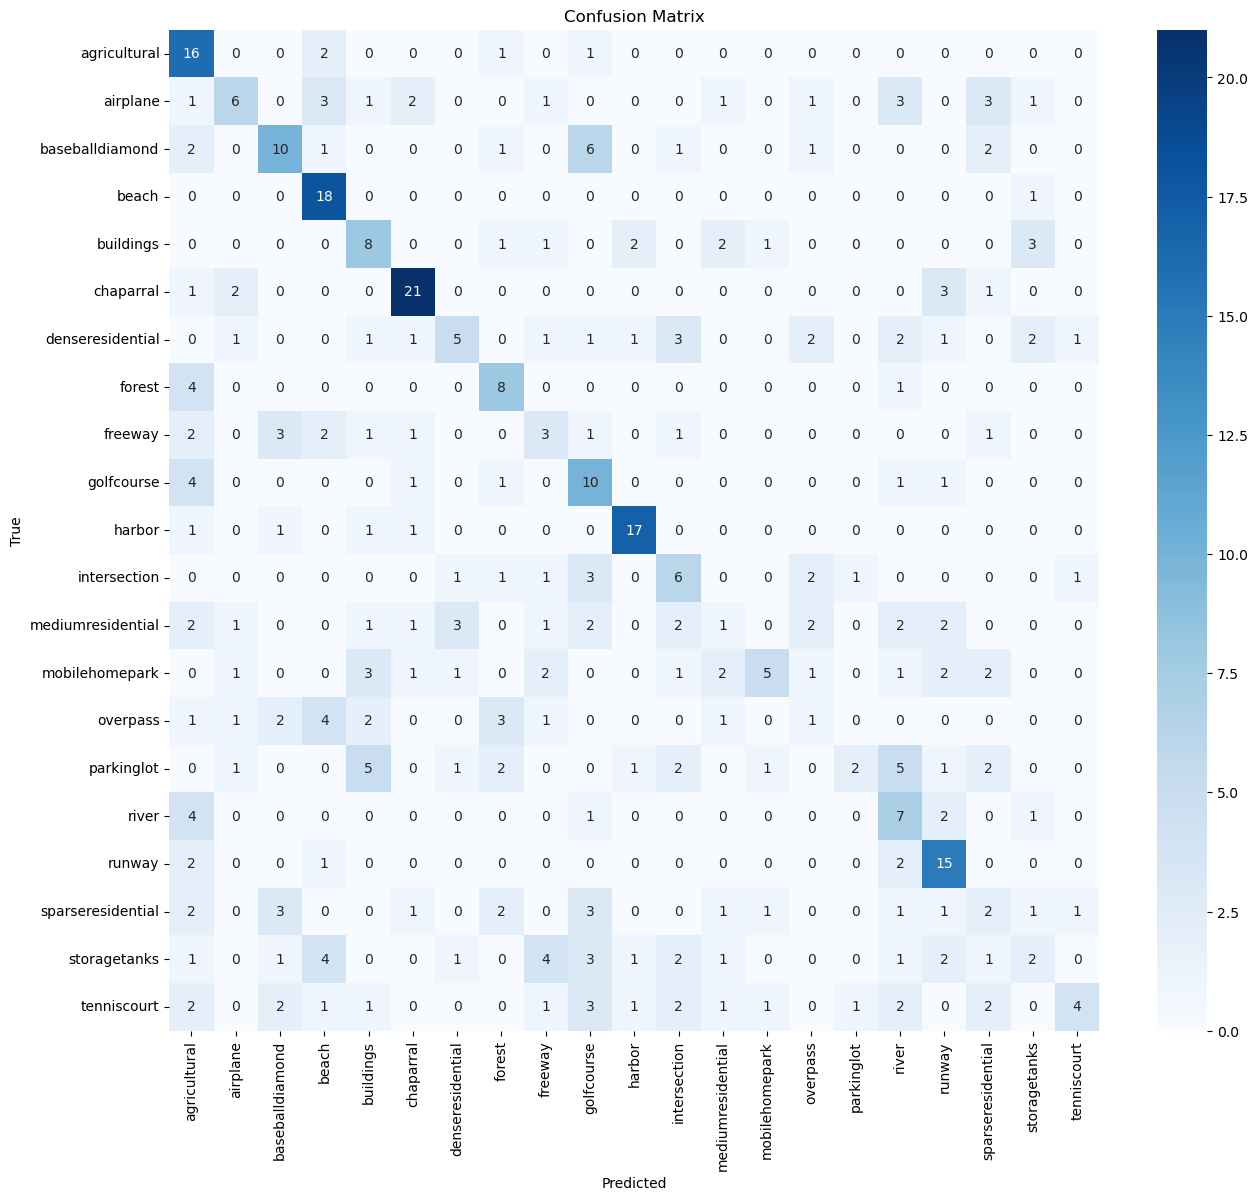
\includegraphics[width=0.5\textwidth]{Figures/methods/confusion_matrix.pdf}
    \caption[Concept of Confusion Matrices]{Conceptual representation of a confusion matrix, depicting the relationship between the predicted values and labels (actual values), adapted from \autocite{Fawcett2006}.}
    \label{fig:conf_matrix}
\end{figure}

%%%%%%%%%%
\subsubsection*{\glsentrylong{oa}}

\gls{oa} measures the proportion of correctly classified predictions out of the total predictions. It is a general measure of how well a classifier performs across all classes \autocite{Moharram.Sundaram2023,Zhao.Tu.ea2023}. It is calculated by dividing the sum of the \gls{tp} and \gls{tn} predictions by the sum of all predictions. The formula for \gls{oa}, used by the \emph{TorchMetrics} package \autocite{Torchmetrics2024a}, is described as
\begin{equation}
    \text{\gls{oa}} = \frac{1}{n}\sum_{i=1}^n 1(y_i = \hat{y}_i),
\end{equation}
whereas \( n \) is the total number of samples, \( y_i \) is the true label for the \( i \)-th sample, \( \hat{y}_i \) is the predicted label for the \( i \)-th sample, and \( 1(y_i = \hat{y}_i) \) is an indicator function that equals one if \( y_i = \hat{y}_i \), so when the prediction is correct, otherwise results to zero.

An alternative depiction of this formula including the aforementioned terms, seen in according literature like in \textcite{Tzepkenlis.Marthoglou.ea2023,Zhao.Tu.ea2023}, is
\begin{equation}
    \text{\gls{oa}} = \frac{\gls{tp} + \gls{tn}}{\gls{tp} + \gls{tn} + \gls{fp}+ \gls{fn}}.
\end{equation}

\gls{oa} should be used with caution, especially when the classes are highly imbalanced, because it can be misleading in such cases. For example, it can increase in cases where the accuracy of a class increases more than it decreases of another class \autocite{Chicco.Jurman2020,Powers.Ailab2011}. By solely looking at the \gls{oa}, this imbalanced behavior cannot be detected, which is why additional metrics are needed to evaluate the model's performance more accurately.

%%%%%%%%%%
\subsubsection*{\glsentrylong{ca}}

Because of the limitations of \gls{oa}, \gls{ca} is used as an additional metric to split the \gls{oa} into each class. It measures the proportion of correctly classified predictions for them \autocite{Fawcett2006}. A confusion matrix, as shown above, shows the class-wise accuracy, but for multiple model runs, averaging these values is done by using the arithmetic mean
\begin{equation}
    \text{\gls{ca}} = \sum_{i=1}^n \frac{\gls{tp}_i}{n},
\end{equation}
whereas \( n \) is the total number of model runs and \( \gls{tp}_i \) the \gls{tp} for the \( i \)-th sample/model run.

By looking at specific classes, conclusions about the used \gls{osm} filters can be drawn in addition to possible issues with the input data. For example, if the model has a high accuracy for the class \emph{built-up}, but a low accuracy for the class \emph{grass}, it can be assumed that the \gls{osm} filter for \emph{grass} contains contradictory \gls{osm} tags or that the input data is not sufficient for the model to extract all the information needed to correctly predict the class. The \gls{ca}, therefore, is more accurate for evaluating the accuracy of imbalanced datasets than the \gls{oa}. 

%%%%%%%%%%
\subsubsection*{\( F_{1} \) Score}

Another common performance evaluation metric is the \( F_{1} \) score. It is the harmonic mean of precision and recall, two metrics to measure the proportion of \glspl{tp} in relation to the sum of certain types of predictions. Precision measures the exactness of a model, so how many of the \glspl{tp} are actually \gls{tp}. On the other hand, recall measures the model's completeness, so how many of all as positive predicted classes were correctly predicted \autocite{Hu.Li.ea2020,Mi.Chen2020,Mohammed.Kora2023,Zhao.Tu.ea2023}. The \( F_{1} \) score is calculated by dividing the product of precision and recall by the sum of precision and recall. A high \( F_{1} \) score near one indicates a good precision and recall, and a low value towards zero indicates the opposite. Basically, the \( F_{1} \) score measures the model's accuracy, but differently than \gls{oa}, for it takes into account how the data is distributed, therefore suitable for imbalanced data \autocite{Chicco.Jurman2020,Mi.Chen2020,Powers.Ailab2011,Zhao.Tu.ea2023}.

It should be reported alongside the \gls{oa} to get a better understanding of the model's performance. This approach enhances the evaluation of both balanced and imbalanced data. Unfortunately, by using the \enquote{multiclass} parameter in the \emph{TorchMetrics} package, the result is exactly the same as \gls{oa}. Regarding these both, this results in ignoring the \( F_{1} \) score and only using the \gls{oa} for the results report.

%%%%%%%%%%
\subsubsection*{\glsentrylong{iou}}

The \gls{iou}, or as it is also sometimes called, the Jaccard Index or Jaccard Similarity Coefficient, is a metric that measures the overlap between the predicted output and the ground truth, divided by the combined area of both \autocite{Csurka.Larlus2013,Demir.Musaoglu2023}. It is defined as
\begin{equation}
    J(A,B) = \frac{|A\cap B|}{|A\cup B|} = \frac{\gls{tp}}{\gls{tp} + \gls{fp} + \gls{fn}} = \text{\gls{iou}},
\end{equation}
whereas \( A \) is the predicted output and \( B \) the ground truth \autocite{Demir.Musaoglu2023,Torchmetrics2024b}.

Using the \enquote{multiclass} parameter, this metric is applied to each class separately and then averaged to get the overall \gls{iou} value. That is why this actually is the mean \gls{iou}, as showed in \textcite{Minaee.Boykov.ea2022,Zhao.Tu.ea2023}. The (mean) \gls{iou} value lies between 0 (no overlap between predicted value and label) and 1 (perfect overlap between predicted value and label). It functions as an alternative measurement of the accuracy and is particularly useful when the location of the prediction matters, for it compares segmentation patches with each other and not only classification values \autocite{Chicco.Jurman2020,Mi.Chen2020}.

%%%%%%%%%%
\subsubsection*{Loss \& Accuracy Progression}

Finally, the loss progression in comparison to the accuracy progression can also be used as a performance metric. As explained in section \ref{subsec:loss}, the loss function is used to optimize the model's parameters during training, so the loss should decrease over time, while the accuracy should increase. Monitoring these for the training and validation sets, the models can be checked for their fitting behavior, and, therefore, the reliability of the other metrics and the overall training process.

%%%%%%%%%%
\subsection{Resource Consumption \& Efficiency}

A model can be using a lot of resources, having a high resource consumption, but still be efficient in its performance when utilizing these resources effectively. This means that if a model is using a lot of resources, but also has a high performance, it can be considered efficient, although a low resource consumption paired with a high performance would be even more efficient, of course. On the other hand, a model can be using a lot of resources, but still have a low performance, which would make it inefficient. Resource consumption and efficiency of a model are important to monitor, because they can tell if a model run is successful in reducing resource consumption while still achieving high performance \autocite{Li.Jiang.ea2021,Xu.Zhou.ea2021}.

The consumption of energy, the emission of carbon, and the overall efficiency solely of the model are difficult to monitor without additional precautions and hardware. \textcite{Mehlin.Schacht.ea2023} introduce different tools for this task, but point out that these tools oftentimes provide only an estimation and have to be reported alongside the geographic region and its infrastructure. Even then, a direct comparison and evaluation, for example of the carbon emission, is still imprecise. In addition to that, the accuracy of the model should also always be included, because achieving a lower energy consumption but also a lower accuracy, for example, is not a good trade-off \autocite{Li.Jiang.ea2021,Tao.Meng.ea2022}. Furthermore, if a code-dependent tool is used, the energy consumption can vary depending on the code and the machine it is running on \autocite{Mehlin.Schacht.ea2023}. Nevertheless, there are some metrics that can be used to estimate the resource consumption and efficiency of the model, which are described below.

%%%%%%%%%%
\subsubsection*{Runtime \& Number of Epochs}

The primary metrics for assessing a model's resource consumption and efficiency are its runtime and the number of epochs required for convergence. These metrics are a reliable indication, as long as the same hardware and software settings are used \autocite{Mehlin.Schacht.ea2023}. However, as explained also in section \ref{subsec:regularization}, less epochs or a shorter runtime do not necessarily mean a more efficient model. A shorter runtime and comparable performance imply higher efficiency, while a higher number of epochs and a longer runtime imply a higher resource consumption regardless of the performance. Similarly, a low resource consumption alongside low performance are not a good trade-off and not efficient as well. The model's total runtime serves as a indicator of its overall resource consumption, as longer runtimes typically correlate with a higher energy consumption \autocite{Li.Jiang.ea2021,Xu.Zhou.ea2021}. To enhance comparability, the time needed per epoch is calculated as well, enabling a better understanding of the model's efficiency in comparison to the performance.

%%%%%%%%%%
\subsubsection*{Model Size}

As showed in \textcite{Mehlin.Schacht.ea2023,Tao.Meng.ea2022}, the model size can also be important for the resource consumption of the model. It is usually directly correlated to the complexity of the model, therefore, needed resources to train and infer \autocite{Xu.Zhou.ea2021}.

Additionally, although today a good internet connection and enough disk space are not a rarity anymore, handling and distributing models with multiple hundreds or thousands of MB can still have an indirect impact on the model's resource consumption. The framework of the \gls{lulcu} is designed to offer an online storage of the model, so the larger the model, the more space is required on the server and cloud which themselves burn a lot of energy to offer this service. By keeping the model size low, these indirect resource consumptions can be reduced. The model size is automatically measured in MB and is the space taken up by the model on the online storage.

%%%%%%%%%%
\subsubsection*{Energy Consumption}

Regarding energy consumption, the \gls{lulcu} has an energy tracker from the \emph{pyJoules} package \autocite{PowerAPI2024} implemented, which measures the consumed energy in Millijoules. But, a large drawback of the measurement is, that it is not possible to monitor the energy consumption of the model alone. The tracker measures the energy consumption of the whole machine in its current state, which includes the main parts \gls{cpu}, \gls{ram}, and \gls{gpu}, but also cooling systems and drives, all drastically influenced by running software and the unoptimized harmonization of hardware. Running a machine with as few additional programs in the background as possible helps in getting a more accurate measurement of the model's energy consumption, but it will never be the exact amount the model has consumed. \textcite{Li.Jiang.ea2021,Mehlin.Schacht.ea2023} present other tools for energy consumption measurement as well, but all have similar drawbacks and limitations.

Because additional hardware for measuring energy could not be installed on the machine and the comparability could not be given due to the setup, this measurement is disregarded and replaced with the following one.

%%%%%%%%%%
\subsubsection*{Hardware Utilization}

Measuring the energy consumption of hardware parts without hardware-near tools is much harder than measuring their utilization, therefore, this is monitored instead. The \gls{cpu}, \gls{gpu} and its memory (\gls{vram}), as well as the \gls{ram} utilization, are measured during the model run and their maxima and averages compared. The largest focus is on the \gls{gpu}, for this part is mainly used for training the model and the largest consumer on the machine, as shown above in table \ref{tab:hardwareconfig}. Additionally, because the \gls{cpu} is the second largest consumer and also highly involved in successfully training the model, it is monitored alongside the \gls{gpu}. \gls{ram} and \gls{vram} play a minor role, because there should be a linear relationship between larger feature spaces and higher memory utilization. That is why reducing the complexity of the road network, as explained in the extension sections, is important. Still, their utilization is monitored to check for memory leaks or other issues, possibly explaining other performance or efficiency issues. 

As measuring the energy consumption, the utilization of those parts can also be influenced by running software in the background. However, the monitoring is much more detailed with more tools at hand, therefore, using the same machine configuration for all the runs and minimizing background processes, the utilization should still give better tendencies on how much the model uses the hardware resources. This gives an good estimation on how difficult it is to train the model and how much computational power is needed, giving a good insight into the resource consumption of the models.

%%%%%%%%%%
\subsubsection*{Carbon Emission}

Finally, measuring the carbon emission depends on the energy source mix of the geographical location which the machine uses \autocite{Mehlin.Schacht.ea2023}. Because this is difficult to determine, the carbon emission is not measured additionally in this study. \textcite{Li.Jiang.ea2021} suggest using a \enquote{Greenness} score for evaluating the carbon emissions of the model, but this was redeemed unfeasible for the task at hand, because it consists of multiple energy measurements, which are disregarded. The presented metrics are good indicators for the efficiency and resource consumption of the different extensions to the model, therefore, carbon emissions will not be included in this assessment.

\chapter{Results}
\label{sec:results}

Three research questions have been put up in the context of the hypothesis, that \enquote{by adding information about the spatial context of \gls{lulc} classes using a road network, the model convergence should be supported and the overall resource consumption reduced alongside an increase of the accuracy, as the model can make more informed decisions about the \gls{lulc} classes}.

The second research question, \emph{\enquote{what is a suitable encoding method to integrate them into the feature space of the model}}, has been answered in the methodology chapter, partly based on the results regarding the first research question. Road types are reduced in their complexity beforehand by using a \gls{hca} and merging road types with similar relationships over \gls{lulc} classes, and speed limits are feature engineered by merging multiple \gls{osm} tags together and categorizing the values into fixed speed limit ranges. Both attributes are encoded via \gls{ohe} and integrated into the feature space of the \gls{lulcu}.

Their suitability for the task at hand is shown by analyzing their relationship to \gls{lulc} classes, fully answering the first research question \emph{\enquote{which attributes of the \gls{osm} road network can provide the model spatial contextual information regarding \gls{lulc} classes, and what is their relationship to adjacent \gls{lulc} classes derived from \gls{osm}}}.

Finally, the third research question, \emph{\enquote{how much does the integrated road network and its attributes impact the model's performance and resource consumption}}, is also answered in this chapter by presenting the results of the model runs and analyzing them.

%%%%%%%%%%
\section{Relationship Between Roads \& \glsfmtshort{lulc} Classes}

\emph{RQ 1: Which attributes of the \gls{osm} road network can provide the model spatial contextual information regarding \gls{lulc} classes, and what is their relationship to adjacent \gls{lulc} classes derived from \gls{osm}?}

In order to give an answer to this question, the results of the explorative relationship analysis between road network attributes and \gls{lulc} classes is presented. The analysis is divided into two sections according to the two attributes of the road network types and speed limits, respectively.

%%%%%%%%%%
\subsection{Road Types vs. \glsfmtshort{lulc} Classes}

This section presents the results of the relationship analysis between road types and \gls{lulc} classes. The analysis is split into two parts: assessing the relationship visually and statistically.

%%%%%%%%%%
\subsubsection*{Visual Relationship}
\label{subsec:vis}

Figure \ref{fig:types_lulc_vis} visualizes the distribution of four out of the 16 road types shown in table \ref{tab:roadlengths}. They are plotted on top of the \gls{lulc} classes before feature engineering them as explained in section \ref{sec:ext2}. The remaining road types are shown in appendix section \ref{app:vis_lulc}.

\begin{figure}[!htb]
    \centering
    \includegraphics[width=\textwidth]{Figures/maps/Single Road Types main.pdf}
    \caption[Visual Relationship between Select Road Types and \glsfmtshort{lulc} Classes]{Visual Relationship between select road types and \gls{lulc} classes for \gls{mahdrnk}. Additional road types are found in appendix section \ref{app:vis_lulc}. Colors represent \gls{lulc} classes, whereas \enquote{built-up} is red, \enquote{forest} is green, \enquote{water} is blue, \enquote{farmland} is yellow, \enquote{permanent\_crops} is orange, and \enquote{grass} is light green (as in figure \ref{app_fig:lulc} in appendix section \ref{app:aoi}). Roads are black.}
    \label{fig:types_lulc_vis}
\end{figure}

The figures primarily show that the occurrence and density of specific road types is highly heterogeneous. Some road types cover nearly the full \gls{aoi}, the high share of over 41 \% of the \emph{track} roads is clearly visible, while others are either very distributed or barely represented. Both links of \emph{motorway} and \emph{trunk} (figure \ref{app_fig:types_lulc_vis_maj}) and types \emph{cycleway} and \emph{pedestrian} (figure \ref{app_fig:types_lulc_vis_min}), all with a share of the total road network length of under 1 \%, are barely visible, making it difficult to draw conclusions about their spatial relationship to \gls{lulc} classes. All in all, the road network is more dense on the western part of the \gls{aoi} and sparse in the southeast.

The major road types, including \emph{motorway, trunk, primary, secondary}, and \emph{tertiary}, are distributed across all \gls{lulc} classes, although \emph{primary} seems to rather occur in built-up areas and \emph{motorway} rather in farmlands. The same applies for \emph{path} and \emph{unclassified}, although both are very granulated, \emph{unclassified} more than \emph{path}. \emph{Path} is more distributed over all \gls{lulc} classes, \emph{unclassified} seems to rather avoid forest areas. Types \emph{footway} and \emph{service} are quite similar in their spatial distribution, whereas \emph{service} covers more area, as it has a higher share.

Some roads seem to be bound to specific \gls{lulc} classes. \emph{Footway, living\_street, residential}, and \emph{service} seem to occur rather in built-up areas, whereas \emph{track} seems to avoid built-up areas completely. It is noticeable that \emph{track} and \emph{residential} are nearly the opposite of each other. Interestingly, \emph{path} is not similar to \emph{track}, although the first impression would suggest that. Forest areas are usually avoided, except for \emph{track} and \emph{path}, although only \emph{track} roads cover nearly all forest areas. Farmlands usually have a sparse network, except for \emph{track} and some roads of the major road types.

So, at first glance, it seems that the road types \emph{residential, footway, living\_street}, and \emph{service} are bound to built-up areas, while \emph{track} is the opposite. The other road types do not seem to have a preference for a specific \gls{lulc} class. This will be investigated further in the statistical relationship analysis.

%%%%%%%%%%
\subsubsection*{Statistical Relationship}

The relationship between road types and \gls{lulc} classes is further analyzed statistically. The results are presented in two heatmaps, showing the distribution of road types over \gls{lulc} classes and vice versa (see figure \ref{fig:types_mean}). The heatmaps are based on the total road length per road type and \gls{lulc} class, respectively. They are the averages of the applied buffers as explained in section \ref{subsec:explore} and as shown in figure \ref{app_fig:types_lulc_v} and \ref{app_fig:types_lulc_h} in the appendix section \ref{app:road_types}. The according figures and the changes between them are not explained in detail, because for the model it only is important to see if there are differences in the signals between the road types for the \gls{lulc} classes. It is sufficient to say that the buffers do have an impact on the distribution, but the average pattern represents the distributions well.

Figure \ref{fig:types_v_mean} shows the quantified relative distribution of road types over \gls{lulc} classes. As explained in section \ref{subsec:explore}, the shares of the total road length per road type have been calculated per \gls{lulc} class, so the figure shows which roads are more prevalent in each \gls{lulc} class, based on the total road length in each \gls{lulc} class. The highest values are achieved by \emph{track}, covering over 70 \% of farmlands, forests, and permanent crops, as well as over 54 \% of grass. \emph{Residential} has the highest share in built-up areas with 30.4 \%, \emph{path} in water areas with 28.4 \%, followed by \emph{track} with 23.5 \%. A strong relation between road types and \gls{lulc} classes (over 50 \%) is only visible for the road type \emph{track} for the three mentioned \gls{lulc} classes as well as permanent crops.  

Peculiarities are that 16.2 \% of built-up areas are intersecting with \emph{track}, which was not observable in the visual relationship, as well as the four types \emph{path, track, footway}, and \emph{service} near water areas, which also was not observable in the figure due to the small share of water areas in the \gls{aoi} (1.7 \%). Also, although \emph{service} has a high share in the road network (11.3 \%), only slightly less than \emph{residential} (14.2 \%), it has not a similar relation to built-up like \emph{residential}, it is more distributed towards water with otherwise similar values in the other \gls{lulc} classes.

\begin{figure}[htb]
    \centering
    \begin{subfigure}{0.4625\textwidth}
        \centering
        \includegraphics[width=\textwidth]{Figures/results/road_types/lulc/road_types_lulc_vertical_mean.png}
        \caption{Heatmap of Road Types per \gls{lulc} Class.\\Summation to 100 \% vertically.}
        \label{fig:types_v_mean}
    \end{subfigure}
    \begin{subfigure}{0.5275\textwidth}
        \centering
        \includegraphics[width=\textwidth]{Figures/results/road_types/lulc/road_types_lulc_horizontal_mean.png}
        \caption{Heatmap of \gls{lulc} Classes per Road Type.\\Summation to 100 \% horizontally.}
        \label{fig:types_h_mean}
    \end{subfigure}
    \caption[Averaged Heatmaps of Road Types vs. \glsfmtshort{lulc} Classes]{Heatmaps showing the relationship between road types and \gls{lulc} classes, averaged over all buffer sizes (0, 10, 25 m; see appendix section \ref{app:road_types}). The distribution depends strongly on the share of road types (A) and the area of \gls{lulc} classes (B) in the \gls{aoi}. All values under 1 \% are omitted for clarity, summation includes the omitted values.}
    \label{fig:types_mean}
\end{figure}

Because of the high share of \emph{track} roads (41.3 \%), the other road types have mostly low distribution values, so the figure is quite biased and, therefore, not very informative about the relationship between road types and \gls{lulc} classes, except those mentioned. That is why for this data no \gls{hca} was conducted, as it would not provide any additional information other than \emph{track} being largely different from the other road types.

In order to get a better understanding of the relationship between road types and \gls{lulc} classes, the distribution is turned around. In figure \ref{fig:types_h_mean}, the share of \gls{lulc} classes adjacent to the road types is shown, summing up to 100 \% horizontally based on the total road length of each road type. In this figure, the distribution gets more distinct. The prior very prevalent road type \emph{track} has now a differentiated distribution over the \gls{lulc} classes, having its highest intersection with the forest class with 37.5 \%, but falling under 1 \% in the water class and under 10 \% in the classes built-up and permanent crops.

The only road types whose largest share (over 50 \%) intersects with a specific \gls{lulc} class are \emph{footway, living\_street, pedestrian, residential}, and \emph{service}, which are the most prevalent in the built-up class. This was also already shown in the \gls{hca} in section \ref{sec:ext2}, where \emph{living\_street, pedestrian}, and \emph{residential} road types were merged together into one class. These three have an even higher relation to built-up areas than \emph{footway} and \emph{service} with each over 70 \%, whereas the other two are between 60 and 65 \%. No other road type intersects over 50 \% with a \gls{lulc} class, only \emph{motorway\_link} does so with the grass class just below at 49.5 \%.

The other road types have a more diverse distribution over the \gls{lulc} classes. There are not many types whose share is the largest in one specific \gls{lulc} class except for those mentioned above, but some road types split themselves over two or three specific \gls{lulc} classes. \emph{Cycleway, motorway\_link, primary, secondary, trunk}, as well as \emph{trunk\_link} all have more than 25 \% of them distributed over the \gls{lulc} classes built-up and grass.  

As assumed in section \ref{sec:ext2}, the major road classes are distributed differently over the \gls{lulc} classes, therefore not merging them in one class was the right decision. Especially \emph{tertiary} and \emph{unclassified} differ from the others with their largest shares distributed over the three \gls{lulc} classes built-up, forest, as well as grass, and built-up, farmland, and grass, respectively. The largest share of \emph{track} are distributed over farmland, forest, and grass, with its largest (37.5 \%) over forest.

For the other merged road types, \emph{motorway, trunk}, and their links, the relationships differ in some aspects. \emph{Motorway} and \emph{trunk} are similar for their largest share intersects with grass, but differ for their second and third largest share intersect oppositely with built-up and forest. \emph{Trunk} and its link seem very similar, but \emph{motorway} and its link have a large difference in the grass class, with the link having a share of 49.5 \%, whereas \emph{motorway} has only 32.5 \%. It seems that the link is more prevalent in grass areas and the \emph{motorway} in forest. The distributions of these road types could provide unclear signals to the model.

Comparing these values with the shares of \gls{lulc} classes in the \gls{aoi}, stronger relationships can be seen. Although forest has a share of 39.6 \% of all \gls{lulc} classes, only \emph{motorway, path}, and \emph{trunk} intersect to over 25 \% with it. Contrary, although grass only has a share of 7.7 \%, \emph{cycleway, motorway, motorway\_link, primary, secondary, trunk}, and \emph{trunk\_link} all intersect with it over 25 \%, suggesting a stronger relationship. Water is even more underrepresented than in the other figure, as its share is only 1.7 \%. Additionally, although farmlands have a share of 30.6 \%, no road type intersects with it over 25 \%. And, although built-up areas have a smaller share of 18.3 \%, many road types intersect with it over 25 \%.

In order to compare the pattern similarities of the road types to determine if specific signals for the \gls{lulc} classes exist for the model to train on, a \gls{hca} has been conducted based on these results, as explained in section \ref{sec:ext2}. Figure \ref{fig:types_clustermap} combines the two distinct figures, the heatmap in figure \ref{fig:types_mean} and the dendrogram in figure \ref{fig:types_dendrogram_mean} into a clustermap, enabling the fast comparison of similar patterns of road types and \gls{lulc} classes.

The first thing that catches the eye is that the most of the largest shares of road types are in the built-up and grass classes, although not always above 50 \%. Additionally, \emph{motorway, path}, and \emph{track} have a large intersection with forest. For farmlands, only \emph{track} has a large share. Permanent crops and water have only have shares under 10 \%.

When looking on the left dendrogram, which shows similar patterns of road types, there are two major groups, splitting into the ones stronger associated with built-up and those with a more distributed pattern, as seen above. They are further split into smaller groups, based on their distributions over specific \gls{lulc} classes. For the model, it would mean that there are primarily signals to better distinguish between built-up and not built-up areas, but also between grass and forest areas. The other two \gls{lulc} classes are not as distinct, therefore it is expected, that for these \gls{lulc} classes the performance will not be enhanced as much.

\begin{figure}[htb]
    \centering
    \includegraphics[width=.9\textwidth]{Figures/results/road_types/clustering/road_types_lulc_dendrogram_mean.png}
    \caption[Clustermap of Road Types vs. \glsfmtshort{lulc} Classes]{Clustermap showing the hierarchical clustering of road types, averaged over all buffer sizes (0, 10, 25 m; see figure \ref{app_fig:types_dendrograms}) based on their distribution pattern similarity over \gls{lulc} classes (see figure \ref{fig:types_h_mean}). The left dendrogram shows the clustering of the road types, the top dendrogram the clustering of the \gls{lulc} classes. The nearer the lines of the dendrograms to the heatmap, the more similar the patterns (unitless).}
    \label{fig:types_clustermap}
\end{figure}

Looking at the top dendrogram, which shows the pattern similarity between \gls{lulc} classes, this assumption is confirmed. Most similar are water and permanent crops, then farmland and forest, grass is more different than these two groups together, and built-up the most different. For the model it would mean that it gets signals it can interpret, but their effectivity depends on the \gls{lulc} class.

Because the clustermap is also influenced by the imbalanced \gls{lulc} classes, a \gls{ppmc} analysis has been conducted as well in order to see if \gls{lulc} classes correlate with each other in their relationship to road types, regardless of the length of road types or the area of \gls{lulc} classes. Figure \ref{fig:pmcc_types_mean} shows the result of this analysis, again averaged for all buffer sizes. A positive relationship near 1 means that the classes are strongly linearly related to each other, a negative relationship near -1 that they are strongly opposed, and values around 0 impose a missing linear relationship.

\begin{figure}[htb]
    \centering
    \includegraphics[width=.66\textwidth]{Figures/results/road_types/lulc/road_types_lulc_correlation_mean.png}
    \caption[\glsfmtshort{ppmc} of \glsfmtshort{lulc} Classes Based on Road Types]{\gls{ppmc} of \gls{lulc} classes based on road type distribution, averaged over all buffer sizes (0, 10, 25 m; see figure \ref{app_fig:types_correlation}). Asterisks show according the significance level at 0.05 (*), 0.01 (**), and 0.001 (***), respectively. The upper triangle is omitted for clarity.}
    \label{fig:pmcc_types_mean}
\end{figure}

The \gls{ppmc} confirms that there are linear relationships between the \gls{lulc} classes, with the strongest positive one between farmland and permanent crops, and the strongest negative one between forest and built-up, as assumed in the elaborations above.

Interestingly, there is nearly no relationship between grass and farmlands, which is surprising, as they are both partially agricultural areas (\emph{landuse=meadow} in grass class). Also surprising is the relatively strong relation between forest and farmland as well as permanent crops. This shows that there is a relationship between agricultural areas and forests based on the road network in them. Unsurprising is the negative relationship between built-up and all other classes, as this has been shown in all figures above.

So, all in all, it seems that road types can give the model according signals towards adjacent \gls{lulc} classes, although not every class will be strongly positively impacted by the integration of the road types into the feature space of the \gls{lulcu}.

%%%%%%%%%%
\subsection{Speed Limit Classes vs. \glsfmtshort{lulc} Classes}

This section focuses on the relationship between speed limits and \gls{lulc} classes, the second attribute of the road network that is investigated. Because of the many missing values, the visual relationship analysis is skipped. The statistical relationship is analyzed similarly to the road types by using two heatmaps, a \gls{hca}, and the \gls{ppmc} analysis, showing the distribution of speed limit classes over \gls{lulc} classes and vice versa (see figure \ref{fig:speeds_mean}). Similar to analyzing the road types, the heatmaps are based on the total road length per speed limit class and \gls{lulc} class, respectively. They are the averages of the applied buffers as explained in section \ref{subsec:explore} and as shown in figure \ref{app_fig:speeds_v} and \ref{app_fig:speeds_h} in the appendix section \ref{app:speeds}. As previously, the according figures and changes between them are not explained in detail. The buffers also affect the distribution in this case, yet the average pattern adequately reflects the distributions as well.

\begin{figure}[htb]
    \centering
    \begin{subfigure}{.465\textwidth}
        \centering
        \includegraphics[width=\textwidth]{Figures/results/speeds/speeds_lulc_vertical_mean.png}
        \caption{Heatmap of Speed Limit Classes per \gls{lulc} Class.\\Summation to 100 \% vertically.}
        \label{fig:speeds_v_mean}
    \end{subfigure}
    \begin{subfigure}{.525\textwidth}
        \centering
        \includegraphics[width=\textwidth]{Figures/results/speeds/speeds_lulc_horizontal_mean.png}
        \caption{Heatmap of \gls{lulc} Classes per Speed Limit Class.\\Summation to 100 \% horizontally.}
        \label{fig:speeds_h_mean}
    \end{subfigure}
    \caption[Averaged Heatmaps of Speed Limit Classes vs. \glsfmtshort{lulc} Classes]{Heatmaps showing the relationship between speed limit classes and \gls{lulc} classes, averaged over all buffer sizes (0, 10, 25 m; see appendix section \ref{app:speeds}). The distribution depends strongly on the share of speed limit classes (A) and the area of \gls{lulc} classes (B) in the \gls{aoi}. All values under 1 \% are omitted for clarity, summation includes the omitted values.}
    \label{fig:speeds_mean}
\end{figure}

Figure \ref{fig:speeds_v_mean} shows the relative distribution of the speed limit classes over \gls{lulc} classes. As explained in section \ref{subsec:explore}, the shares of the total road length per speed limit class have been calculated per \gls{lulc} class analog to the procedure for the road types, so the figure shows which roads are more prevalent in each \gls{lulc} class, based on the total road length in each \gls{lulc} class.

Quite noticeable is the one high value of 72 \% in the relation between the speed limit class \enquote{very low} and the built-up \gls{lulc} class. \enquote{Very low} has the highest share in the road network with over 56 \%, explaining its highest prevalence in every \gls{lulc} class except water. The second highest share of the road network has the speed limit class \enquote{low} with nearly 20 \%, which explains why it has high shares over the \gls{lulc} classes as well. Interestingly, it intersects the most with water areas, surpassing even the class \enquote{very low}. Although \enquote{very high} has the third largest share of the road network with 8.55 \%, it is the second most prevalent speed limit class in farmlands and forests, suggesting an even stronger relationship towards these \gls{lulc} classes. \enquote{Medium}, with 6.3 \% the fourth largest share of the network, is usually the fourth largest share in all \gls{lulc} classes as well except for built-up. The other speed limit classes have low values, with \enquote{high} and \enquote{walk} having the lowest shares in the road network, observable in this figure.

The assumption relating the speed limit classes is, that the further outside of cities, the higher the speed limit. Because of the imbalanced shares of speed limit classes this assumption can not be confirmed by only using this figure, that is why the figure next to it, figure \ref{fig:speeds_h_mean}, is consulted. In this figure, again the share of \gls{lulc} classes adjacent to the speed limit classes is shown, summing up to 100 \% horizontally based on the total road length of each speed limit class.

Partially confirming the assumption, the largest shares of the three slowest speed limit classes \enquote{walk}, \enquote{very low}, and \enquote{low} intersect with the built-up class. But, nearly one quarter of each of the two fastest speed limit classes \enquote{very high+} and \enquote{unlimited} intersect with built-up also, showing a opposite distribution as expected. In both of them, the other shares mainly split over the forest and grass classes, although \enquote{very high+} has a shifted distribution with less of its roads in the \gls{lulc} class forest and more in grass.

As before, due to the low shares of water and permanent crops, they are underrepresented. Additionally, only the speed limit class \enquote{unlimited} has a share of over 5 \% intersecting with water areas, all other classes are below. The higher mid range speed limits \enquote{high} and \enquote{very high} have a more distributed pattern over the three \gls{lulc} classes farmland, forest, and grass.

\begin{figure}[htb]
    \centering
    \includegraphics[width=.75\textwidth]{Figures/results/speeds/clustering/speeds_lulc_dendrogram_mean.png}
    \caption[Clustermap of Speed Limit Classes vs. \glsfmtshort{lulc} Classes]{Clustermap showing the hierarchical clustering of speed limit classes, averaged over all buffer sizes (0, 10, 25 m; see figure \ref{app_fig:speeds_dendrograms}) based on their distribution pattern similarity over \gls{lulc} classes (see figure \ref{fig:speeds_h_mean}). The left dendrogram shows the clustering of the speed limit classes, the top dendrogram the clustering of the \gls{lulc} classes. The nearer the lines of the dendrograms to the heatmap, the more similar the patterns (unitless).}
    \label{fig:speeds_clustermap}
\end{figure}

The figures show a diverse distribution, although the assumption, that lower speed limits are more prevalent in built-up areas and higher speed limits in rural areas, is partially confirmed. However, a linear pattern is not clearly observable, as the highest speed limit classes have a high share in built-up areas as well. All speed limit classes intersect with the \gls{lulc} class grass, although the lower speed limits less than the faster ones. Farmlands and forests are mainly intersected by the mid range speed limits, especially \enquote{high} and \enquote{very high}. 

The \gls{hca} in figure \ref{fig:speeds_clustermap} shows the pattern similarities of the speed limit classes. As the figure shows in the left dendrogram, the speed limit classes are mainly clustered into two groups, one with the slowest speed limits \enquote{walk}, \enquote{very low}, and \enquote{low}, and the other with the faster speed limits. The most similar pattern have \enquote{walk} and \enquote{very low} with the highest share (over 70 \%) of each in built-up areas and the second highest in grass. \enquote{Low} has also a similar pattern, but with a higher share in grass and a lower share in built-up.

Interestingly, \enquote{unlimited} is more similar to \enquote{medium} than to \enquote{very high} and \enquote{high}, and these two more to \enquote{very high+} than to the other two high speed classes \enquote{very high} and \enquote{high}. \enquote{Unlimited} and \enquote{medium}, therefore, break up the assumption than high speed limits are found outside of built-up areas.

The top dendrogram shows that the \gls{lulc} classes are clustered into two groups as well, one with the built-up class and the other with the other five classes, similar to the road types. The highest similarity have water and permanent crops, but this is not representative due to their small share of the total \gls{lulc} area, as explained above. Farmland and forest seem more related to each other than to grass, repeating the pattern seen in the road types, although in this case grass belongs to the same subgroup.

The \gls{ppmc} confirms that there are linear relationships between the \gls{lulc} classes, with the strongest positive one, contrary to the road types, between forest and grass, closely followed by farmland and forest, and the strongest negative one at a significant -0.98 between forest and built-up, taking the statement of the road type analysis a step further. The correlation matrix generally looks different from the one for the road types, in general intensifying relations shown in the road types, like between built-up and the classes farmland, forest, and grass, also between forest and farmland, and between grass and forest. Surprising differences are especially in permanent crops and grass, which now have a positive relation, contrary to their prior negative relation with the same strength. Also, there is a relation between farmland and grass now, which was not observable before. Unsurprising is the negative relationship between built-up and all other classes, similar to the road types, as this has been shown in all figures above.

So, all in all, it seems that speed limits also can give the model signals towards adjacent \gls{lulc} classes, but the signals are different from those of the road types. Some relations are similar and stronger, others opposite, so not every class will be strongly positively impacted by the integration of the speed limit classes into the feature space of the \gls{lulcu}.

\begin{figure}[htb]
    \centering
    \includegraphics[width=.66\textwidth]{Figures/results/speeds/speeds_lulc_correlation_mean.png}
    \caption[\glsfmtshort{ppmc} of \glsfmtshort{lulc} Classes Based on Speed Limit Classes]{\gls{ppmc} of \gls{lulc} classes based on speed limit class distribution, averaged over all buffer sizes (0, 10, 25 m; see figure \ref{app_fig:speeds_correlation} in appendix section \ref{app:road_types}). Asterisks show the according significance level at 0.05 (*), 0.01 (**), and 0.001 (***), respectively. The upper triangle is omitted for clarity.}
    \label{fig:pmcc_speeds_mean}
\end{figure}

For Extension 4, the merge of both encodings, it is expected that the context inclusion will have a strong impact on built-up, as there are strong signals from both road types and speed limits. For the other classes, the impact is expected to be less strong, possibly even negative, as the signals might be contradictory, reducing the clarity of signals towards \gls{lulc} classes.

%%%%%%%%%%
\section{Model Evaluation}

\emph{RQ 3: What is the impact of the integrated road network and its attributes on the model's performance and resource consumption?}

In section \ref{subsec:metrics}, multiple metrics have been presented in order to answer this question. The aim of this is to evaluate how the different extensions perform in comparison to the baseline runs and whether integrating a road network has a positive or negative impact on the performance and/or resource consumption of the model, if there is any. This should show if this approach is feasible and build the basis for further studies regarding spatial contextual information inclusion. The section above, where the results of the explorative relationship analysis between the road network attributes and \gls{lulc} classes were presented, showed that there are signals the model could utilize to make more informed predictions. The following evaluation will show if the model can make use of these signals and if the signals are strong enough to enhance the model's performance or provide useful information to increase its efficiency.

The following sections present the metrics of the different models. Note that in all following tables, some cells are colored to enhance the perception. Depending on the metric, either the highest or the lowest value is the best. Usually for performance metrics, the higher the better, and the opposite for resource consumption metrics. The according best one will be marked green, and the according worst value will be colored yellow. Additionally, each cell will have an arrow indicating its performance in comparison to the baseline, which is an average of the three baseline runs. The arrows show the direction of the difference (increase/decrease), and the color the according rating (better/worse), as used for rating the best and worst value. The numbers of channels of each extension are added to the first two result tables to show their complexity in addition to the metrics for clarity. In subsequent tables, these will be omitted to reduce the table size.

%%%%%%%%%%
\subsection{Overview over Resource Consumption \& Efficiency}

Before diving into the two metric groups and specific metrics, the general metrics of the model runs are presented in table \ref{tab:eval_overview} in an overview manner, showing first efficiency estimations. The assumption for the three general resource consumption metrics number of epochs, runtime, and model size, is, the lower the values, the lower the resource consumption, regardless of the performance of the model runs. The opposite is assumed for the performance metrics \gls{oa} and \gls{iou} of the test phases, also shown in this table. The time needed per epoch is added for comparability, as it is dependent the number of epochs and the runtime. 

\begin{table}[htb]
    \centering
    \caption[Overview over General Model Run Metrics]{Overview over the general performance (test sets) and resource consumption metrics for all model runs. The baseline runs are averaged and the extension runs compared to this average. The assumption for the resource consumption metrics number of epochs, runtime, and model size is, the lower the values, the lower the resource consumption. The opposite is assumed for the performance metrics \gls{oa} and \gls{iou}. Time per epoch is added for comparability. In green the best value per metric and in yellow the worst (if baseline runs are one of them, the according extension run is colored as well). The arrows show the direction of the difference (increase/decrease).}
    \begin{adjustbox}{center}
        \begin{tabular}{cccccccc}
            \toprule
            \textbf{Model Run} & \textbf{Channels} & \textbf{Epochs} & \textbf{Runtime [s]} & \textbf{Time/Epoch [s]} & \textbf{Size [MB]} & \textbf{\gls{oa} [\%]} & \textbf{\gls{iou} [\%]} \\
            \midrule
            Baseline 1 & 5 & 37 & 691 & \best 18.68 & 83.01 & \best 76.69 & 36.42 \\
            Baseline 2 & 5 & 13 & \best 269 & 20.69 & 30.79 & 71.85 & 34.24 \\
            Baseline 3 & 5 & 28 & 536 & 19.14 & 65.28 & 66.34 & 29.68 \\
            \midrule
            Baseline & 5 & 26 & 498.67 & \best 19.50 & 59.69 & 71.63 & 33.45 \\
            \midrule
            Extension 1.1 & 6 & \worst 43 \upbad & 1030 \upbad & \best 23.95 \upbad & \worst 115.58 \upbad & 72.57 \upgood & 37.24 \upgood \\
            Extension 1.2 & 6 & 13 \downgood & \best 348 \downgood & 26.77 \upbad & 35.55 \downgood & 70.74 \downbad & 35.34 \upgood \\
            Extension 1.3 & 6 & 25 \downgood & 609 \upbad & 24.36 \upbad & 68.02 \upbad & 68.86 \downbad & 38.68 \upgood \\
            \midrule
            Extension 2.1 & 16 & 29 \upbad & 1444 \upbad & 49.79 \upbad & 40.47 \downgood & 68.90 \downbad & 37.42 \upgood \\
            Extension 2.2 & 16 & 16 \downgood & 826 \upbad & 51.63 \upbad & 20.98 \downgood & 70.56 \downbad & \best 39.29 \upgood \\
            Extension 2.3 & 16 & 22 \downgood & 1099 \upbad & 49.95 \upbad & 29.62 \downgood & 72.62 \upgood & 37.44 \upgood \\
            \midrule
            Extension 3.1 & 13 & 16 \downgood & 703 \upbad & 43.94 \upbad & 21.26 \downgood & 69.73 \downbad & 34.02 \upgood \\
            Extension 3.2 & 13 & 16 \downgood & 680 \upbad & 42.50 \upbad & 21.73 \downgood & 69.37 \downbad & 33.80 \upgood\\
            Extension 3.3 & 13 & \best 12 \downgood & 535 \upbad & 44.58 \upbad & \best 16.43 \downgood & \worst 64.31 \downbad & \worst 28.27 \downbad \\
            \midrule
            Extension 4.1 & 24 & 20 \downgood & 1405 \upbad & \worst 70.25 \upbad & 24.54 \downgood & \best 74.63 \upgood & 38.61 \upgood \\
            Extension 4.2 & 24 & 33 \upbad & \worst 2231 \upbad & 67.61 \upbad & 38.41 \downgood & 66.20 \downbad & 37.01 \upgood\\
            Extension 4.3 & 24 & 23 \downgood & 1583 \upbad & 68.83 \upbad & 27.00 \downgood & 68.01 \downbad & 38.14 \upgood \\
            \bottomrule
        \end{tabular}
    \end{adjustbox}
    \label{tab:eval_overview}
\end{table}

The first thing to notice is that the baselines are neither the best nor the worst in all metrics. They have the lowest runtime, lowest time per epoch, and the highest \gls{oa} score, but the other metrics are dominated by the extensions, especially the \gls{iou}, where only Extension 3.3 achieves a lower value than all baseline runs, and the number of epochs needed for convergence, where only three of the twelve extension runs needed more epochs than the baseline. Extension 4.2 has the longest runtime with 2231 s, more than triple the longest baseline run, and Extension 1.2 the shortest with 348 s, which is shorter than two of the baseline runs. The model size has a very high variability between 16.43 MB by Extension 3.3 and 115.58 MB by Extension 1.1, with the baselines ranging in between. The \gls{oa} scores range between the highest value by Baseline 1 with 76.69 \% and the lowest by Extension 3.3 with 64.31 \%. The \gls{iou} scores are closer together, with the highest value achieved by Extension 2.2 with 39.29 \%, better than all baseline runs, and the lowest by Extension 3.3 with 28.27 \%, worse than all baseline runs.

In order to put the values into perspective, the fitting behavior of the model runs, monitored by comparing the loss of the training and validation phases and rating the curve progressions, is shown in figure \ref{fig:losses}. As the step count is not equalized, the curves are not directly comparable, but the general behavior can be observed and rated.

\begin{figure}[!hp]
    \centering
    \begin{subfigure}{.325\textwidth}
        \centering
        \includegraphics[width=\textwidth]{Figures/results/extensions/loss/15_loss.png}
        \caption{Baseline 1.\\Good fitting.}
    \end{subfigure}
    \begin{subfigure}{.325\textwidth}
        \centering
        \includegraphics[width=\textwidth]{Figures/results/extensions/loss/14_loss.png}
        \caption{Baseline 2.\\Overfitting.}
    \end{subfigure}
    \begin{subfigure}{.325\textwidth}
        \centering
        \includegraphics[width=\textwidth]{Figures/results/extensions/loss/13_loss.png}
        \caption{Baseline 3.\\Moderate fitting.}
    \end{subfigure}
    \\
    \begin{subfigure}{.325\textwidth}
        \centering
        \includegraphics[width=\textwidth]{Figures/results/extensions/loss/12_loss.png}
        \caption{Extension 1.1.\\Slightly Overfitting.}
    \end{subfigure}
    \begin{subfigure}{.325\textwidth}
        \centering
        \includegraphics[width=\textwidth]{Figures/results/extensions/loss/11_loss.png}
        \caption{Extension 1.2.\\Good fitting.}
    \end{subfigure}
    \begin{subfigure}{.325\textwidth}
        \centering
        \includegraphics[width=\textwidth]{Figures/results/extensions/loss/10_loss.png}
        \caption{Extension 1.3.\\Slightly overfitting.}
    \end{subfigure}
    \\
    \begin{subfigure}{.325\textwidth}
        \centering
        \includegraphics[width=\textwidth]{Figures/results/extensions/loss/9_loss.png}
        \caption{Extension 2.1.\\Good fitting.}
    \end{subfigure}
    \begin{subfigure}{.325\textwidth}
        \centering
        \includegraphics[width=\textwidth]{Figures/results/extensions/loss/8_loss.png}
        \caption{Extension 2.2.\\Good fitting.}
    \end{subfigure}
    \begin{subfigure}{.325\textwidth}
        \centering
        \includegraphics[width=\textwidth]{Figures/results/extensions/loss/7_loss.png}
        \caption{Extension 2.3.\\Slightly overfitting.}
    \end{subfigure}
    \\
    \begin{subfigure}{.325\textwidth}
        \centering
        \includegraphics[width=\textwidth]{Figures/results/extensions/loss/6_loss.png}
        \caption{Extension 3.1.\\Moderate fitting.}
    \end{subfigure}
    \begin{subfigure}{.325\textwidth}
        \centering
        \includegraphics[width=\textwidth]{Figures/results/extensions/loss/5_loss.png}
        \caption{Extension 3.2.\\Moderate fitting.}
    \end{subfigure}
    \begin{subfigure}{.325\textwidth}
        \centering
        \includegraphics[width=\textwidth]{Figures/results/extensions/loss/4_loss.png}
        \caption{Extension 3.3.\\Overfitting.}
    \end{subfigure}
    \\
    \begin{subfigure}{.325\textwidth}
        \centering
        \includegraphics[width=\textwidth]{Figures/results/extensions/loss/3_loss.png}
        \caption{Extension 4.1.\\Moderate fitting.}
    \end{subfigure}
    \begin{subfigure}{.325\textwidth}
        \centering
        \includegraphics[width=\textwidth]{Figures/results/extensions/loss/2_loss.png}
        \caption{Extension 4.2.\\Good fitting.}
    \end{subfigure}
    \begin{subfigure}{.325\textwidth}
        \centering
        \includegraphics[width=\textwidth]{Figures/results/extensions/loss/1_loss.png}
        \caption{Extension 4.3.\\Moderate fitting.}
    \end{subfigure}
    \caption[Loss Plots of Model Runs]{Loss of the training (blue) and validation (orange) phase for each model run. As the number of epochs is not equalized, the comparability between the model runs is limited. The fitting behavior is categorized in good, moderate, and overfitting.}
    \label{fig:losses}
\end{figure}

All training curves show an overall decrease, which means that they all achieved convergence. Some models did not perform well and overfitted the data, and some other models even have lower validation than training loss. This can be due to data augmentation and regularization techniques used in training and not in validation or having a too small validation set, which then happens to be an \enquote{easier} dataset to predict. Nevertheless, as the curves decrease and follow similar patterns, they signify successful model runs. Their different fitting behavior is mirrored in table \ref{tab:eval_overview}, which shows that all groups incorporate a high variability between their runs. Nevertheless, the models are all included in the comparison as they all have a similar fitting behavior in general per extension group and use the same overall dataset, architecture, and hyperparameters, which means they all have the same limitations.

Averaging the values per baseline and extension, respectively, ensures better comparability and seems feasible based on the high variability in every group around a somewhat average-like medium model. Therefore, from this point on, only the averaged metrics will be analyzed in regard to the research question, where the extension groups are more important rather than single model runs for evaluating the extensions' impact on the model's performance and resource consumption. It should kept in mind that for all metrics, the variability is high. The metrics of all model runs are found in the appendix section \ref{app:evaluation}. Additionally, the plotted curves of the performance metrics \gls{oa} and \gls{iou} for the training and validation phases for each model run can be found in the appendix sections \ref{app:acc} and \ref{app:iou}, respectively, as well. These will also not be discussed here and function only as verification for claimed results.

Continuing in table \ref{tab:eval_avg}, the metrics from table \ref{tab:eval_overview} are averaged per extension and compared to the baseline. As seen here, the main tendencies in comparison to the baseline do not change much, but it is clearer now that the extensions perform differently among themselves. Extension 3 is interesting for it has the lowest resource consumption values, but also the worst performance metrics. As the time per epoch also is much higher than the baseline or even Extension 1, it has a low efficiency and provides a bad trade-off between performance and resource consumption, signifying a failed attempt to enhance the model. Extension 4, on the other hand, has the worst runtime and time per epoch, but performs comparably good, achieving the second best \gls{iou}. This also is a bad trade-off, as achieving comparable performance with higher computational costs is a failed enhancing attempt as well. Extension 1 and 2 seem to achieve better results, as they perform better than the baseline in regard to \gls{iou} and comparable in \gls{oa} (less than 1 \% lower), while having higher computational costs. So, they achieve an increase in performance with increased computational costs, a usual trade-off.

\begin{table}[htb]
    \centering
    \caption[Grouped General Model Run Metrics]{General performance (test sets) and resource consumption metrics grouped and averaged by extension, compared to the baseline.}
    \begin{adjustbox}{center}
        \begin{tabular}{cccccccc}
            \toprule
            \textbf{Extension} & \textbf{Channels} & \textbf{Epochs} & \textbf{Runtime [s]} & \textbf{Time/Epoch [s]} & \textbf{Size [MB]} & \textbf{\gls{oa} [\%]} & \textbf{\gls{iou} [\%]}\\
            \midrule
            Baseline & 5 & 26 & \best 498.67 & \best 19.18 & 59.69 & \best 71.63 & 33.45 \\
            \midrule
            Extension 1 & 6 & \worst 27.00 \upbad & 662.33 \upbad & \best 24.51 \upbad & \worst 73.05 \upbad & \best 70.72 \downbad & 37.09 \upgood \\
            Extension 2 & 16 & 22.33 \downgood & 1123.00 \upbad & 50.29 \upbad& 30.36 \downgood & 70.69 \downbad & \best 38.05 \upgood \\
            Extension 3 & 13 & \best 14.67 \downgood & \best 639.33 \upbad & 43.58 \upbad & \best 19.81 \downgood & \worst 67.81 \downbad & \worst 32.03 \downbad \\
            Extension 4 & 24 & 25.33 \downgood & \worst 1739.67 \upbad & \worst 68.68 \upbad & 29.98 \downgood & 69.61 \downbad & 37.92 \upgood \\
            \midrule
            Extensions & - & 22.08 \downgood & 1066.08 \upbad & 48.28 \upbad & 38.05 \downgood & 69.71 \downbad & 36.75 \upgood \\
            \bottomrule
        \end{tabular}
    \end{adjustbox}
    \label{tab:eval_avg}
\end{table}

Interestingly, the number of epochs and the model size of all extensions are much lower except for Extension 1. Similarly, all \gls{iou} values are higher than the baseline except for Extension 3. Comparing these values to the complexity of the models derived from the number of channels, it is difficult to observe a linear relationship between complexity and resource consumption or performance. Model sizes and epochs, for example, both are the worst in Extension 1 and best in Extension 3, but for Extension 2 and 4, the increase/decrease relation is turned around, giving a example against a linear relationship.

Evaluating the model runs solely on these metrics is not enough to make final statements about the impact of the road attributes on the model. Therefore, the following sections will dive deeper into the according metrics to better evaluate the impact of the integrated road network and its attributes on the model.

%%%%%%%%%%
\subsection{Performance}

Looking further into the performance of the models, the maximal \gls{oa} and \gls{iou} values for each phase of the model training process are shown in table \ref{tab:performance_avg}. The prior tendencies are changed completely, as the extensions perform nearly always better than the baseline, except for the \gls{oa} in the test phase, of course. There are single exceptions in every phase metric, usually in Extension 3, which performs worse in four of six metrics compared to the baseline, but the extensions usually perform better than the baseline in all other cases, usually in four to five out of the six cases.

Extension 4 has the highest values in the training and validation phases in both metrics, which makes sense compared to it being the most complex extension with the highest runtime. Although Extension 1 is less complex than Extension 3, it still achieves better performance in all cases except \gls{iou} during validation, while having a slightly longer runtime. Extension 2, being the second most complex extension and also having the second longest runtime, achieves always the second best value of the extension except for the \gls{iou} in the test phase, where it surpasses Extension 4. Without Extension 3, a linear relationship is visible, where the metrics increase the higher the complexity, but as Extension 3 has the worst values and the \gls{iou} in the test phase of Extension 4 is lower than Extension 2, this assumption cannot be considered valid.

\begin{table}[htb]
    \centering
    \caption[Grouped Maximal Performance Metrics]{Maximal achieved values for \gls{oa} and \gls{iou} in all three phases, grouped and averaged by extension. The full table for all model runs can be found in table \ref{app_tab:performance}.}
    \begin{adjustbox}{center}
        \begin{tabular}{cccccccc}
            \toprule
            \textbf{Model Run} & \textbf{Train \gls{oa} [\%]} & \textbf{Val \gls{oa} [\%]} & \textbf{Test \gls{oa} [\%]} & \textbf{Train \gls{iou} [\%]} & \textbf{Val \gls{iou} [\%]} & \textbf{Test \gls{iou} [\%]} \\
            \midrule
            Baseline & 66.46 & \worst 68.52 & \best 71.63 & 35.10 & 35.37 & 33.45 \\
            \midrule
            Extension 1 & 66.92 \upgood & 69.94 \upgood & \best 70.72 \downbad & 36.40 \upgood & \worst 34.55 \downbad & 37.09 \upgood \\
            Extension 2 & 68.34 \upgood & 73.69 \upgood & 70.69 \downbad & 37.63 \upgood & 39.84 \upgood & \best 38.05 \upgood \\
            Extension 3 & \worst 65.86 \downbad & \worst 69.77 \upgood & \worst 67.81 \downbad & \worst 34.82 \downbad & 36.55 \upgood & \worst 32.03 \downbad \\
            Extension 4 & \best 68.36 \upgood & \best 75.53 \upgood & 69.61 \downbad & \best 38.19 \upgood & \best 40.44 \upgood & 37.92 \upgood \\
            \midrule
            Extensions & 67.37 \upgood & 72.48 \upgood & 69.71 \downbad & 36.26 \upgood & 38.05 \upgood & 36.52 \upgood \\
            \bottomrule
        \end{tabular}
    \end{adjustbox}
    \label{tab:performance_avg}
\end{table}

In addition to comparing the maximal values achieved by the extensions, table \ref{tab:performance_epochcut_avg} shows the metrics at step 13, the lowest number of epochs needed for convergence in the baseline runs (see table \ref{tab:eval_overview}). This allows for the evaluation of performance at identical steps, under the premise that the models were ultimately exposed to the same amount of data for learning.

\begin{table}[htb]
    \centering
    \caption[Grouped Performance Metrics at Step 13]{\gls{oa} and \gls{iou} values at step 13, grouped and averaged by extension. The full table for all model runs can be found in table \ref{app_tab:performance_epochcut}.}
    \begin{adjustbox}{center}
        \begin{tabular}{ccccc}
            \toprule
            \textbf{Model Run} & \textbf{Train \gls{oa} [\%]} & \textbf{Val \gls{oa} [\%]} & \textbf{Train \gls{iou} [\%]} & \textbf{Val \gls{iou} [\%]} \\
            \midrule
            Baseline & \worst 61.98 & \worst 57.24 & \worst 31.71 & \worst 27.26 \\
            \midrule
            Extension 1 & \worst 63.78 \upgood & 64.77 \upgood & \worst 33.05 \upgood & \worst 30.93 \upgood \\
            Extension 2 & \best 65.83 \upgood & \best 66.07 \upgood & 35.59 \upgood & \best 35.32 \upgood \\
            Extension 3 & 64.54 \upgood & \worst 62.96 \upgood & 33.67 \upgood & 33.46 \upgood \\
            Extension 4 & 65.63 \upgood & 65.34 \upgood & \best 35.64 \upgood & 34.45 \upgood \\
            \midrule
            Extensions & 64.95 \upgood & 64.79 \upgood & 34.49 \upgood & 33.54 \upgood \\
            \bottomrule
        \end{tabular}
    \end{adjustbox}
\label{tab:performance_epochcut_avg}
\end{table}

Surprisingly, the baseline has the worst values in all phases and for both metrics, often by a magnitude of multiple percent points (\%p) difference to the lowest performing extension. As for the best performing extension at step 13, Extension 2 achieves the best values in all phases except in the \gls{iou} during the training phase, where it performs only slightly worse than Extension 4. Extension 1 performs the worst among the extensions, with the exception of the \gls{oa} during the validation phase, where only Extension 3 performs worse. The extensions perform better than the baseline in all cases without exception, but, as the time per epoch metric in table \ref{tab:eval_avg} shows, they all will have consumed more resources at step 13 than the baseline. Yet, the better performance is a good trade-off, showing the potential of the extensions to at least enhance the model's performance based on the same amount of data.

As \gls{oa} and \gls{iou} are merged metrics, calculated using all values of the confusion matrices, the averaged \gls{tp} values for each \gls{lulc} class are shown in table \ref{tab:ca_avg}. These values represent the \gls{ca} metric, which helps in comparing class-wise performance. The according confusion matrices of which the \gls{ca} is derived from can be found in the appendix section \ref{app:conf_matrices}.

\begin{table}[htb]
    \centering
    \caption[Grouped \glsentrylong{ca}]{\gls{ca} values of the test phases, grouped and averaged by extension. The full table for all model runs can be found in table \ref{app_tab:ca} in appendix section \ref{app:performance}. Also, the according confusion matrices can be found in appendix section \ref{app:conf_matrices}.}
    \begin{tabular}{ccccccc}
        \toprule
        \textbf{Extension} & \textbf{Built-up} & \textbf{Forest} & \textbf{Water} & \textbf{Farmland} & \textbf{Permanent Crops} & \textbf{Grass} \\
        \midrule
        Baseline & \worst70.33 & 84.33 & \worst78.00 & 69.00 & \worst43.00 & \best41.33 \\
        \midrule
        Extension 1 & 82.00 \upgood & 84.67 \upgood & 86.33 \upgood & \best 74.00 \upgood & \worst 51.00 \upgood & 34.67 \downbad \\
        Extension 2 & 86.00 \upgood & 84.00 \downbad & \best 91.67 \upgood & 68.33 \downbad & 56.67 \upgood & \best 39.33 \downbad \\
        Extension 3 & \worst 79.00 \upgood & \best 87.00 \upgood & \worst 84.00 \upgood & \worst 57.00 \downbad & 53.33 \upgood & \worst 20.33 \downbad \\
        Extension 4 & \best 87.67 \upgood & \worst 82.67 \downbad & 90.67 \upgood & 64.33 \downbad & \best 67.00 \upgood & 37.33 \downbad \\
        \midrule
        Extensions & 83.67 \upgood & 84.59 \upgood & 88.17 \upgood & 66.67 \downbad & 57 \upgood & 32.92 \downbad \\
        \bottomrule
    \end{tabular}
    \label{tab:ca_avg}
\end{table}

The extensions perform better than the baseline in four of the six \gls{lulc} classes, except farmland and grass. The baseline then again performs best in the \gls{lulc} class grass, and worst in the classes built-up, water, and permanent crops. As shown above, the relationship between the road attributes were the most evident towards the built-up class, which experiences a considerable increase in prediction accuracy in all extensions. The same applies to the classes water and permanent crops. In the forest class, extensions and baseline perform similarly. In the grass class, all models achieve a performance below 50 \%, the extensions averaged even under 33 \%, making it by far the worst predicted class. Interestingly, integrating only the road network without further data (Extension 1) already improves the prediction of all \gls{lulc} classes except grass.

The extensions perform similarly in the farmland class, where the \gls{ca} is worse than the baseline except in Extension 1, which outperforms the baseline by 5 \%. However, the average \gls{ca} of the extensions is over 65 \%, therefore, the overall prediction is much better than in the grass class. The class permanent crops also has a subpar \gls{ca} in the baseline with 43 \%, but the extensions achieve a considerable increase in performance, especially Extension 4, which achieves by far the highest value in this class with 67 \%. Interestingly, every extension performs the best in one of the classes, although Extension 4 holds the highest value in the two classes built-up and permanent crops. Because of this distribution, a linear relationship between complexity and performance again cannot be detected, as the most complex extension does not perform the best in all classes. The only extension which performs better than the baseline while all other extensions perform worse is Extension 1 in the farmland class.

Extensions predict water the best, followed by forest and built-up, although the range of \gls{ca} differs in them. Of these three, forest has the smallest variation with 4.33 \%p, then water with 7.67 \%p, and finally built-up with the largest variation of 8.67 \%p. The other three classes, which are predicted worse, also have a much higher variability between 16 \%p in permanent crops to 19 \% in grass. This shows that the model is more stable in predicting the classes water, forest, and built-up, while the other classes are more difficult to predict and have a higher variability in the predictions.

%%%%%%%%%%
\subsection{Hardware Utilization}

Although some resource consumption metrics have already been explored in regard to the research question, the utilization of the hardware components is analyzed below, replacing energy consumption and carbon emission measurements. Again, all following tables show averaged values per extension group for better comparability with the baseline. 

Because they are the two highest consumers in the machine, the utilization of \gls{gpu} and \gls{cpu} is looked into first. Their utilization in percent is shown in table \ref{tab:util_major_avg}. Contrary to the values above in table \ref{tab:eval_overview}, the resource consumption in form of hardware utilization seems to be the highest in the baseline, with an exception in Extension 2, which reached a higher maximal \gls{gpu} utilization. However, all cases in the table have a lower utilization, usually more than five \%p, except for the mentioned value and the same metric for Extension 3, which reached the same maximal utilization of the \gls{gpu} as the baseline.

\begin{table}[htb]
    \centering
    \caption[Grouped Hardware Utilization - \glsfmtshort{gpu} \& \glsfmtshort{cpu}]{Average and maximal utilization of \gls{gpu} and \gls{cpu}, grouped and averaged per extension. The values are compared to the baseline. \O{} denotes the average value, and Max the maximum value. The full table for all model runs can be found in table \ref{app_tab:util_major}.}
    \begin{tabular}{cccccc}
        \toprule
        \textbf{Extension} & \textbf{\gls{gpu} \O{} [\%]} & \textbf{\gls{gpu} Max [\%]} & \textbf{\gls{cpu} \O{} [\%]} & \textbf{\gls{cpu} Max [\%]} \\
        \midrule
        Baseline & \worst 19.40 & 64.33 & \worst 32.30 & \worst 78.60 \\
        \midrule
        Extension 1 & \worst 14.37 \downgood & \best 63.00 \downgood & \worst 29.86 \downgood & 71.47 \downgood \\
        Extension 2 & 10.08 \downgood & \worst 66.33 \upbad & 25.71 \downgood & 64.47 \downgood \\
        Extension 3 & 10.90 \downgood & 64.33 & \best 24.07 \downgood & \best 63.87 \downgood \\
        Extension 4 & \best 7.32 \downgood & \best 63.00 \downgood & 24.65 \downgood & \worst 71.83 \downgood \\
        \midrule
        Extensions & 10.67 \downgood & 64.17 \downgood & 26.07 \downgood & 67.91 \downgood \\
        \bottomrule
    \end{tabular}
    \label{tab:util_major_avg}
\end{table}

The expectation would be that the more complex the model, the more are \gls{gpu} and \gls{cpu} utilized. But, the values show a different picture, as the most complex extension, Extension 4, utilized the \gls{gpu} the least both maximal and averaged, and Extension 1 the most averaged. Also, despite having more than the double amount of channels, Extension 3 utilizes the \gls{cpu} less than Extension 1 in both cases, which definitely negates the expectation of a linear increase of hardware utilization with complexity and also its opposite, at least regarding the largest consumers.

\begin{figure}[htb]
    \centering
    \begin{subfigure}{.49\textwidth}
        \centering
        \includegraphics[width=\textwidth]{Figures/results/extensions/gpu.png}
        \caption{Regression Plot of \gls{gpu} Utilization.}
        \label{fig:gpu_reg}
    \end{subfigure}
    \begin{subfigure}{.49\textwidth}
        \centering
        \includegraphics[width=\textwidth]{Figures/results/extensions/cpu.png}
        \caption{Regression Plot of \gls{cpu} Utilization.}
        \label{fig:cpu_reg}
    \end{subfigure}
    \caption[Regression Plots of \glsfmtshort{gpu} \& \glsfmtshort{cpu} Utilization]{Regression plots showing the relationship between number of channels (equates to feature space size and extension type) and average (blue) and maximal (orange) \gls{gpu} (A) and \gls{cpu} (B) utilization.}
    \label{fig:major_reg}
\end{figure}

In order to investigate a possible linear relationship, a regression plot is used, shown in figure \ref{fig:major_reg}, which uses the utilization values of all model runs as seen in table \ref{app_tab:util_major} in appendix section \ref{app:efficiency}. The regression plot shows the relationship between the complexity, denoted as the number of channels, and the average and maximal \gls{gpu} and \gls{cpu} utilization.

As seen in table \ref{tab:util_major_avg}, it is difficult to pinpoint a linear relationship between complexity and hardware utilization. This can be seen in the regression plots as well, as either the variability is high or some extensions behave contrary to a linear relationship. The maximal \gls{gpu} utilization stays on a similar level for all groups, although two runs of Extension 3 with 13 channels have comparably high and low values, respectively. The maximal \gls{cpu} utilization is non-linear, as Extension 2 (16 channels) and 3 both utilize it less than Extension 1 and 4, both with lower and higher complexity, respectively. The \gls{cpu} is utilized in average similarly by Extensions 2 to 4, only the baseline and Extension 1 utilize it more. The average \gls{gpu} utilization is similar for all extensions with a slight negative linearity, although {\nobreak Extension 1} has a higher variability than the other extensions. The baseline utilizes the \gls{gpu} the most. So, a linear relationship is not really present due to a combination of high and missing variability in the runs and between the extensions.

The other two important hardware components for \gls{dl} training, as shown in table \ref{tab:hardwareconfig}, are \gls{ram} and \gls{vram}. The utilization of these two is shown in table \ref{tab:util_minor_avg}. However, contrary to \gls{gpu} and \gls{cpu}, the values are in Gigabytes. This is the first and only table which shows a clear relation between complexity and utilization in all metrics.

The baseline utilizes both \gls{ram} and \gls{vram} the least, while Extension 4 utilizes them the most. Extension 4, also, has a peak \gls{ram} utilization of 28.30 GB, just below to maximal allocation for the \gls{wsl} at 30 GB, as shown in table \ref{tab:hardwareconfig}. Surprisingly, the \gls{vram} utilization peaks just under four GB in Extension 4, which is only half of the maximal allocation of 8 GB.

\begin{table}[htb]
    \centering
    \caption[Grouped Hardware Utilization - \glsfmtshort{ram} \& \glsfmtshort{vram}]{Average and maximal utilization of \gls{ram} and \gls{vram}, grouped and averaged per extension. The values are compared to the baseline. \O{} denotes the average value, and Max the maximum value. The full table for all model runs can be found in table \ref{app_tab:util_minor}.}
    \begin{adjustbox}{center}
        \begin{tabular}{cccccc}
            \toprule
            \textbf{Extension} & \textbf{\gls{ram} \O{} [GB]} & \textbf{\gls{ram} Max [GB]} & \textbf{\gls{vram} \O{} [GB]} & \textbf{\gls{vram} Max [GB]} \\
            \midrule
            Baseline & \best 8.49 & \best 13.97 & \best 2.31 & \best 3.28 \\
            \midrule
            Extension 1 & \best 11.80 \upbad & \best18.63 \upbad & \best 2.42 \upbad & \best 3.28 \\
            Extension 2 & 14.67 \upbad & 24.26 \upbad & 3.01 \upbad & 3.66 \upbad \\
            Extension 3 & 12.32 \upbad & 20.54 \upbad & 2.62 \upbad & 3.50 \upbad \\
            Extension 4 & \worst 17.61 \upbad & \worst 28.30 \upbad & \worst 3.35 \upbad & \worst 3.90 \upbad \\
            \midrule
            Extensions & 14.10 \upbad & 23.43 \upbad & 2.85 \upbad & 3.59 \upbad \\
            \bottomrule
        \end{tabular}
    \end{adjustbox}
    \label{tab:util_minor_avg}
\end{table}

In order to see if the assumed linear relationship exists here, a similar regression plot is used as well as for the other two components, shown in figure \ref{fig:minor_reg}. It is based on the utilization values of all model runs as seen in table \ref{app_tab:util_minor} in appendix section \ref{app:efficiency}.

As expected, the regression lines show a rising regression line between feature space size and memory utilization for both \gls{ram} and \gls{vram}. However, contrary to the average values in table \ref{tab:util_minor_avg}, the linear relationship is not as clear as expected, as the regression lines show a large variability. Especially in the average utilization values of both components, Extension 1 with 6 channels seems to break up the linearity, particularly in comparison to Extension 3 with 13 channels. Also, the step between the baseline and Extension 1 is large in both average and maximal \gls{ram} utilization, but opposing small in the \gls{vram} utilization. However, when leaving out Extension 1, the values show a linear increase in utilization of \gls{ram} and \gls{vram} with increasing complexity.

\begin{figure}[htb]
    \centering
    \begin{subfigure}{.49\textwidth}
        \centering
        \includegraphics[width=\textwidth]{Figures/results/extensions/ram.png}
        \caption{Regression Plot of \gls{ram} Utilization.}
        \label{fig:ram_reg}
    \end{subfigure}
    \begin{subfigure}{.49\textwidth}
        \centering
        \includegraphics[width=\textwidth]{Figures/results/extensions/vram.png}
        \caption{Regression Plot of \gls{vram} Utilization.}
        \label{fig:vram_reg}
    \end{subfigure}
    \caption[Regression Plots of \glsfmtshort{ram} \& \glsfmtshort{vram} Utilization]{Regression plots showing the relationship between number of channels (equates to feature space size and extension type) and average (blue) and maximal (orange) \gls{ram} (A) and \gls{vram} (B) utilization.}
    \label{fig:minor_reg}
\end{figure}

The relationship of hardware utilization for the extensions of \gls{ram} and \gls{vram} can be described as: the larger and more complex the feature space, the higher the \gls{ram} and \gls{vram} utilization. This completely aligns with the assumption stated in section \ref{subsec:machine_config}. Yet, because these two components, particularly the \gls{ram}, do not consume much energy even on full load, their impact on the resource consumption is negligible. As the \gls{vram} is part of the \gls{gpu}, a higher utilization would mean a higher load on the \gls{gpu}, which, however, is not the case as seen above. Still, both components and their utilization show that there is a tendency towards a higher resource consumption with higher complexity, especially when combining these values with the runtime, number of epochs, and time per epoch metrics from table \ref{tab:eval_avg}. The \gls{gpu} and \gls{cpu} follow a opposite pattern in their average utilization, but do not have a linear relationship in their maximal utilization, which is why a concrete statement about the relationship between complexity and hardware utilization cannot be made.

\chapter{Discussion}
\label{sec:discussion}

The study was built around proofing the concept of integrating spatial contextual information into a semantic segmentation model for \gls{lulcm} in order to enhance its performance and resource consumption. Hypothetically, by adding information about the spatial context of \gls{lulc} classes using a road network, the model convergence should be supported and the overall resource consumption reduced alongside an increase of the performance, as the model can make more informed decisions about the \gls{lulc} classes. For this purpose, select attributes of the \gls{osm} road network, road types and speed limits, were encoded and integrated in the feature space of the \gls{lulcu} framework for \gls{lulcm}, which utilizes the SegFormer model for semantic segmentation. This resulted in four extensions, Extension 1 with a boolean road network without further encodings, Extension 2 with encoded road types, Extension 3 with encoded speed limit classes, and Extension 4 with a combination of Extensions 2 and 3. This section discusses the key findings and limitations of the study, implications for future research, as well as giving suggestions for improvement in order to enhance the generalizability and adaptability of the methodology.

%%%%%%%%%%
\section{Key Findings}

The results show that the \gls{osm} road network with its selected attributes road types and speed limits indeed provides spatial contextual information about adjacent \gls{lulc} classes. Integrating roads into the feature space of the model has an impact on the model's performance, resource consumption, and efficiency. In order to enlarge the impact of the road network on the model, the vanilla feature space of the \gls{lulcu} was altered, reducing the satellite imagery based input data from nine bands to five, creating a baseline to compare the results to. The values of the \gls{iou} for the baseline are similar to the performance achieved on the ADE20K and COCO-Stuff benchmark with the SegFormer, shown in the original paper of the SegFormer by \textcite{Xie.Wang.ea2021}. Although not directly comparable, this nevertheless means that even with a reduced feature space, the model still performs well, making the baseline a meaningful comparison basis.

All in all, by integrating road network data into the model, the performance is increased except for select cases, while \gls{gpu} and \gls{cpu} are utilized less, but over a longer runtime. When comparing the \gls{oa} and \gls{iou} of the extensions to the baseline on the same amount of data, the extensions outperform the baseline in all cases, showing that the model can make more informed decisions about the \gls{lulc} classes using the road network. Interestingly, the road geometries alone already increase the performance of the model. As the epochs needed for convergence are reduced in the extensions, they also help the model to converge earlier with less iterations through the data, therefore, the convergence also is supported. However, as the time needed per epoch and runtime are increased considerably for all extensions, even when utilizing \gls{gpu} and \gls{cpu} less, the resource consumption was not improved, meaning that the integration of the road network attributes primarily increases the model's performance while using more resources. The trade-off has to be rated by the possible users and their priority when enhancing models, as the performance and resource consumption do not scale proportionally. 

During the analysis of the results, it became clear that road types have generally a greater positive impact than speed limit classes, as the \gls{oa}, \gls{iou}, and \gls{ca} of the according Extension 2 is generally higher than Extension 3. The only exception is the \gls{lulc} classes forest, where the speed limits achieved a higher \gls{ca}. It should be noted that speed limit classes still improve the performance of the model, although usually to a lesser extent than road types. However, the combination of both road types and speed limits can have an even greater positive impact on the prediction of specific classes, as shown by Extension 4 for the \gls{lulc} classes built-up and permanent crops and the \gls{oa} and \gls{iou} scores for training and validation. But, only three of the six classes experienced an increase in performance in comparison to the other extensions, similar to Extension 2, emphasizing that most of the performance in Extension 4 derives from the road types. This aligns with the assumption stated above, that the speed limit classes will only provide a reduced amount of information, as the majority of the speed limits in the \gls{aoi} is unknown. Still, the impact of the existing speed limits is clearly noticeable, as the performance of the model is increased in the majority of the cases also in Extension 3. Therefore, increasing the complexity and providing as much information as possible does not necessarily lead to better performance, but has the potential to do so if the information has an according density and distribution. However, this comes with the cost of increased resource consumption, as the model has to process more information, which is especially noticeable in the runtime of the model.

According optimization techniques could be applied to reduce the resource consumption, making the model more efficient and sustainable. In section \ref{subsec:training}, the training of \glspl{dnn} was explained and the importance of optimization techniques emphasized. Optimization is one of the biggest challenges of \gls{dl}, as it is necessary in every aspect of the training process. This project was done based on a preset model framework, the \gls{lulcu}, without further adapting possible necessary optimizations for the adapted feature space, both for the baseline as well as for the extensions. Therefore, there is even more potential to be expected regarding the model's performance and efficiency with according tuning of the model's hyperparameters and optimization techniques. But, this has to be evaluated in separate studies, preferably by utilizing the vanilla \gls{lulcu} with its full feature space, as this would show the real potential of the road network as spatial contextual information and enhancement of the model.

%%%%%%%%%%
\section{Road Attributes \& \glsfmtshort{lulc} Classes}

The impact on performance and resource consumption varies between the extensions and the \gls{lulc} classes. The reason for this are the road network attributes utilized in this study themselves. The explorative relationship analysis showed that the tags of the selected attributes have a differentiated relationship towards adjacent \gls{lulc} classes on the one hand. But, the relationship is not as clear as expected on the other hand, as it shows overlaps between features of the attributes in their relationship distribution. Only the minority of the features has a distinct relationship towards only one \gls{lulc} class, most are distributed over multiple classes. Additionally, finding significant relationships or defining thresholds which divide the values into different strengths of relations is difficult without further statistical analyses. But still, the information found in the evaluated relationships still enhance the performance of the model, therefore, for this study, the chosen methodology was suitable.

Furthermore, the results show that the chosen encoding method, \gls{ohe}, was feasible as the information of the features was utilizable by the model. In \gls{ohe}, the features of the road network are rasterized and encoded into boolean tensor channels, which expand the model's feature space. Other encoding methods, including ordinal or binary encoding \autocite{Potdar.Pardawala.ea2017}, could also be utilized if the data meets their requirements, leading to different results for the model, as the values are offered differently to the model to learn from.

Nevertheless, encoding all features of the road network includes many negligible ones, which expand the feature space unnecessary as they do not provide usable information to the model. Also, many features have such a low share in the road network, that including them in the feature space, even when they have a comparably distinct distribution, does not provide the model with a learnable concept or relationship that it can apply for inference, as these roads are barely present in other \glspl{aoi}, for example London, as shown by \textcite{Alghanim.Jilani.ea2021}. This applies for both road types and speed limit classes. Therefore, to reduce the road network's complexity, feature engineering techniques were used. As the model evaluation shows, these were also feasible, as they effectively reduced the number of road types by half and categorized a variable number of different speed limits into 13 fixed categories.

As they are categorized into fixed ranges of speeds based on road classification systems, the categories of the speed limits could be used globally. But, the relationship analysis showed that the categories could be further reduced, as the distribution of the features is not distinct enough to justify the eight categories. This would reduce the complexity of the feature space, so that Extensions 3 and 4 could be more efficient while offering a similar level of information. Mentioned above, the class \enquote{unlimited} is only feasible in Germany and some other minor cases, and as the distribution is similar to \enquote{very\_high+}, these two could be merged. Also, the \gls{hca} showed that \enquote{walk} and \enquote{very\_low} are very similar as well, so merging these too would not reduce the information content of the feature space. Furthermore, the categories are derived from road classification systems of different countries, summarized by \textcite{Vitkiene.Puodziukas.ea2017}. Using a different system could lead to different categories, which could be more distinct or more general, depending on the system and the \gls{lulc} classes to predict. This could also be a way to reduce the complexity of the feature space, as the categories could be more distinct and therefore provide more information to the model. However, their feasibility would have to be evaluated in a separate study and the problem of a low mapping coverage of the speed limits still persists. In order to tackle this, merging multiple datasets with \gls{osm}, for example social media data or measured data from traffic monitoring stations as proposed by \textcite{Camargo.Bright.ea2020,Ludwig.Psotta.ea2023}, could be used to enhance the coverage of the speed limits. This would also enhance the generalizability of the model, as the speed limits would be more representative of the actual speed limits in the \gls{aoi}, maybe evn enhancing the relationship to adjacent \gls{lulc} classes due to their realistic behavior indirectly or directly based on the surrounding \gls{lulc} areas.

As for the road types, the complexity of the features can be reduced further by omitting more road types and by only keeping those with the strongest relation to \gls{lulc} classes, like \emph{residential} and \emph{track}, which both enhance the prediction of built-up areas due to their occurrence and avoidance of these areas, whereby \emph{track} additionally hints towards forests. \textcite{Atwal.Anderson.ea2022} additionally merged the types \emph{primary}, \emph{secondary}, and \emph{tertiary}, but these were not merged in this study due to their different importance in the road network. However, as their distribution over \gls{lulc} classes is similar, they additionally could be merged to reduce the complexity of the feature space. Additionally, increasing the threshold of the global share also reduces the number of road types and helps in generalizing the procedure only to the most important types. The merge of the road types \emph{motorway, trunk}, and their links could be seen as oversimplification, as especially the links have a different distribution than their counterparts. The background for this merge was the applied \gls{lcbb}, whose impact on the model cannot be directly evaluated. As maximal values were used for the buffers, it is possible that road greenery next to roads or grass patches inside and around intersections, like shown in figure \ref{fig:lcbb}, were included in the buffers. This could have a negative impact on the model, as the model could learn to predict roads as grass or vice versa, reducing the accuracy of the grass class.

However, the \gls{ca} of the grass class is already low in the baseline with an accuracy of only 41 \%, so the \gls{lcbb} cannot be the reason for the low performance of the model in the grass class. This probably is based on the reduced feature space and missing satellite imagery, which would be beneficial for the prediction of grass. When comparing the grass to the permanent crops class, which also has a low \gls{ca} of 43 \% in the baseline, there is a large difference in the extensions. The road network enhances the \gls{ca} of the permanent crops class by 8 to 24 \%p, while the performance for the grass class is reduced in all extensions up to 21 \%p, although arguably the performance of Extension 2 is only 2 \%p lower. Looking at the confusion matrices in appendix section \ref{app:conf_matrices}, it is visible that the grass class is confused primarily with the classes permanent crops and farmland, although in some cases forest and built-up are also predicted instead. Orchards, one of the tags of the class permanent crops, are often covered by grass, and farmlands also resemble grasslands in some of their growth states, so the confusion is partially understandable. Even adding vegetation indices as proposed by \textcite{Tzepkenlis.Marthoglou.ea2023} would enhance this prediction only slightly, as the cover is indeed grass. The model predicts the cover correctly, but wrong for the evaluation metric, as the \gls{lulc} class mapped in \gls{osm} is different. Given the additional low \gls{ca} of permanent crops, it is advisable to reconsider the \gls{lulc} classes in order to enhance the model's performance, as these two classes contribute to the lower \gls{oa} compared to the baseline. Suitable \gls{lulc} classes for natural areas could be, for example, forest, bare land, and vegetation, as proposed by \textcite{Basheer.Wang.ea2022}. This would enhance the model's performance, as the classes are more distinct and the model can learn more easily to differentiate between them. The impact of the road network would have to be evaluated separately, as the model has to learn new relationships between the road network and the \gls{lulc} classes.

In that regard, it is to be expected that for different \glspl{aoi}, different shares of the features are present, questioning the generalizability of the model. This is especially true for the road types, as the global distribution of road types is not the same as in the \gls{aoi} of the study. Furthermore, the chosen \gls{aoi} has a characteristic distribution of \gls{lulc} classes and therefore a special relationship between roads and \gls{lulc} classes. The characteristic border between the Odenwald and the Upper Rhine Rift Valley in the \gls{mahdrnk} region provokes a distinct road architecture, avoiding building paved roads in the forested areas with rougher relief and connecting the built-up areas in the valley with more major road types with higher speed limits. But still, as multiple regions with different characteristic distributions were merged into this \gls{aoi}, the overall distribution is representative at least for Germany. All these factors influence the relationship between road types and \gls{lulc} classes. Still, orienting on the global share of the road types is a good basis for reducing the complexity of the according road network to a feasible and utilizable amount.

%%%%%%%%%%
\section{Methodology}

As this study is a proof-of-concept of integrating spatial context into semantic segmentation models to improve the model's performance and efficiency, the concrete relationships between roads and \gls{lulc} classes are only secondary to the overall goal of the study. Nevertheless, the results show tendencies, which are rediscovered analogous in the model evaluation, and by using the road lengths rather than the number of roads, the chosen methodology was generally feasible and sufficient for the task at hand.

The relationships could be explored further in future studies, as the relationships are not as clear as expected and the study only takes into account the relative intersection of roads with adjacent \gls{lulc} classes. The methodology proposed by \textcite{Atwal.Anderson.ea2022} seems more suitable for a more elaborate analysis of the relationship between road networks and \gls{lulc} classes, as it includes a vectorized approach to assess the spatial relationship between the two. These vectors could also be encoded into the feature space of the model to give the model a more detailed understanding of the relationship between roads and \gls{lulc} classes. This would also enhance the generalizability of the model, as the vectors could be applied to different \glspl{aoi} and the model could learn the relationship between roads and \gls{lulc} classes in a more general way. However, to achieve this, the model has to be trained on a much larger dataset, preferably with globally distributed \glspl{aoi}, in order to quantify the relationship realistically and generalized. This would also help in tackling the loss behavior of the models, shown in figure \ref{fig:losses}, where another reason for the lower validation than training loss could be noisy input data and not enough data for a representative validation, which could both be fixed by a larger dataset.

The clustering method to find similarities between the patterns of the explorative relationship analysis in order to reduce the complexity of the road network is based on the \gls{hca}, paired with elaborate feature engineering. This requires domain knowledge and many explicit preprocessing steps. Although suitable for this study, others like k-means and DBSCAN \autocite{Montazeri.Lilienthal.ea2021}, maximum likelihood exploratory factor analysis \autocite{Petrakis.Norman.ea2021}, or the principal component analysis \autocite{Dharani.Sreenivasulu2019} are also proposed as suitable algorithms for effective automated dimensionality reduction. Utilizing them has the potential to offer other insights on the relationships between road attributes and \gls{lulc} classes, enhancing the explorative relationship analysis. However, as \gls{osm} comes with drawbacks like completeness and correctness, feature engineering is required nonetheless to ensure a suitable quality level and a successful utilization of the data. Also, researchers should keep in mind that some information about the \gls{lulc} of the area could be lost if road types are merged together with a not strong enough similarity in their distribution over \gls{lulc} classes. The according task determines the level of detail needed and the most suitable approach.

In that regard, the applied automated feature engineering steps for the road network, including disregarding and merging features as well as filling missing values, are based on domain knowledge, literature, and the \gls{osm} Wiki. However, as \gls{osm} has many anomalies due to wrong mapping, locally restricted information and regional differences \autocite{Ludwig.Fendrich.ea2021}, or even vandalism \autocite{Neis.Goetz.ea2012,Vargas-Munoz.Srivastava.ea2021}, the information of these is lost during this feature engineering procedure, as only few anomalies are included. Although many tools exist to assess the quality of the volunteered \gls{osm} \autocite{Minghini.Frassinelli2019,Moradi.Roche.ea2021,Schott.Zell.ea2024}, researches have to still \enquote{trust} the data of \gls{osm} to some extent. It is advised to base the feature engineering procedure on the \gls{osm} Wiki, where suggested tags and values are summarized, as including every anomaly would require a highly detailed data analysis and a similarly complex feature engineering process.

As for the data itself, the chosen attributes road types and speed limits were selected based on literature and similar studies. Other attributes could be utilized for such a project as well, primarily speed restrictions in specific timeframes or access restrictions. These could also hint towards adjacent \gls{lulc}, for example residential areas when a speed limit is applied only during night time hours or industrial areas where only specific vehicles are allowed. The problem here is the mapping completeness, which is even lower than for the tag \emph{maxspeed} and the speed tags, as well as the low number of occurrences altogether according to \gls{osm} Taginfo. Based on the list of global feature shares and their combinations in \textcite{OSMTaginfo2024}, another idea is to utilize road surface types (tag \emph{surface}), because they also could hint towards specific \gls{lulc} classes. For example, a cobblestone road could be an indicator for a historic city center, while a gravel road could be an indicator for a rural area. The mapping completeness here (25.61 \%) is much higher than for \emph{maxspeed} (7.40 \%) or \emph{access} (6.20 \%), so this could be a possible attribute to utilize. The problem here, on the other hand, is that the distribution of values is more biased, as 44.89 \% of the tag \emph{surface} has the value \emph{asphalt}. The question here, of course, is also if there are similar or even stronger distinct signals between the different features to adjacent \gls{lulc} areas, which is doubtful. A combination of multiple tags can, therefore, be a solution for the bias. However, that would have to be evaluated in a separate study especially in regard to the resource consumption of the model due to the possibly large feature space. Nevertheless, as seen in the evaluation of the extension, the best attribute of the road network to utilize is the road type, as it has the most positive influence on the model's performance and the highest mapping completeness globally, which is further increasing, as shown by \textcite{Anderson.Sarkar.ea2019,Barrington-Leigh.Millard-Ball2017,Herfort.Lautenbach.ea2021}.     

%%%%%%%%%%
\section{Objective \& Data Redundancy}

As mentioned above, this study functions as a proof-of-concept that integrating spatial contextual information enhances \gls{lulcm}. The example of using road networks as according information was chosen based on the idea that they are crucial parts of the landscape and constructed in mind of the adjacent \gls{lulc} areas. But, using roads to classify the adjacent \gls{lulc} areas would be redundant, as \gls{lulc} areas are used for constructing the roads and the roads are then used to classify the \gls{lulc} areas. In other words, it would be a model leakage where the same information is recycled and used again. However, this is based on the assumption that the mapping completeness of the \gls{osm} data is sufficient in the according \glspl{aoi}, regarding both the \gls{lulc} areas as well as the roads. Also, it is based on the assumption that both are correctly mapped, which sometimes is not the case, as \gls{osm} includes many anomalies and is often based on volunteered action, possible with missing domain knowledge. \textcite{Barrington-Leigh.Millard-Ball2017} state that the road network, which is the main emphasis of \gls{osm} (hence the name), usually has a higher mapping completeness than other features, including \gls{lulc}. Also, there is a large bias in mapping completeness of additional features, which concentrate on very densely or sparsely populated areas, as shown by \textcite{Herfort.Lautenbach.ea2021}. Furthermore, utilizing \gls{osm} data always comes with additional drawbacks, including currentness and correctness, which applies also to \gls{lulc} areas.

Yet, as the main task of \gls{ml} models is to utilize learned concepts and models for inference on unknown data \autocite{Sarker2021,Shinde.Shah2018}, completeness is the drawback that has to be tackled the most. In order to tackle the completeness of roads and their attributes in specific \glspl{aoi}, merging data from different sources could be a solution, for example authoritative datasets or the Microsoft Roads dataset, as proposed by \textcite{Anderson.Sarkar.ea2019,Srivastava.VargasMunoz.ea2019,Vargas-Munoz.Srivastava.ea2021}. Moreover, multiple studies introduced \gls{ml} based road type classification algorithms \autocite{Alghanim.Jilani.ea2021,Zhao.Ning.ea2023} using remote sensing and street-view imagery, which, in combination with road detection algorithms \autocite{Abdollahi.Pradhan.ea2020,Chen.Deng.ea2022}, could provide a fully automated \enquote{road detection to \gls{lulcm}} approach. Additionally, average speeds could also be estimated using \gls{dl} approaches, as proposed by \textcite{Keller.Gabriel.ea2020}, further enriching or filling missing data. These methods could tackle the problem of applying this methodology to areas with a low mapping completeness, as roads could be extracted and classified by utilizing \gls{dl} approaches. Both could then be used to enhance the prediction of surrounding \gls{lulc} areas, which in turn could function as a verification for the classified road types. In such cases, utilizing road networks for \gls{lulcm} can provide a real case scenario where \gls{lulcm} of unknown areas can be enhanced with \gls{dl} generated roads. However, such an elaborated approach has to be evaluated in future studies, as the complexity of the model and the resource consumption could increase considerably, providing a bad trade-off between efficiency and performance. In that regard, other model architectures than the SegFormer could also be used for this task, as the SegFormer is not the only model suitable for semantic segmentation. \textcite{Tzepkenlis.Marthoglou.ea2023}, for example, propose a U-Net with a temporal attention encoder, which outperforms the SegFormer in terms of performance and efficiency. In order to measure the efficiency of the according model effectively, \textcite{Desislavov.Martinez-Plumed.ea2023,Getzner.Charpentier.ea2023} propose using Floating Point Operations as a measure of computational complexity, independent from machine configuration. \textcite{Mehlin.Schacht.ea2023} further propose multiple other metrics to measure carbon emission, energy usage, and computational complexity, in order to enhance the evaluation of the model's efficiency and sustainability, which should further be considered in future studies.

All in all, the methodology was suitable for the study and the results show that the integration of spatial contextual information into a semantic segmentation model for \gls{lulcm} is feasible. It enhances the model's performance and offers possible improvements to resource consumption and efficiency, if according optimization techniques are implemented. Therefore, the feasibility of the concept is proven.

\chapter{Conclusion}
\label{sec:conclusion}

This study aimed at evaluating the integration of the \gls{osm} road network and two of its attributes, road types and speed limits, into the feature space of a semantic segmentation model for \gls{lulcm}. Hypothetically, by adding information about the spatial context of \gls{lulc} classes using a road network, the model convergence should be supported and the overall resource consumption reduced alongside an increase of the performance, as the model can make more informed decisions about the \gls{lulc} classes. The feature engineered attributes were encoded via \gls{ohe} into the feature space of the model. The results revealed that this integration provides valuable spatial contextual information about adjacent \gls{lulc} classes, primarily increasing the model's performance while needing less epochs for convergence. Therefore, the model can make more informed decisions about the prediction of \gls{lulc} areas, partially confirming the hypothesis. In four out of six \gls{lulc} classes and five out of six metric comparison cases, the extensions outperform the baseline. This improvement, however, comes at the cost of increased resource consumption and longer runtimes, highlighting a trade-off between enhanced model performance and resource efficiency. Still, the results showed that the model could potentially achieve similar performance with a higher efficiency and less resource consumption, if it is optimized accordingly. The study also highlighted that increasing the complexity of the model by adding more information does not guarantee better performance unless the information is optimized. This finding emphasizes the need for careful consideration of the information included in the model to balance performance gains and resource consumption. Future research should focus on optimizing the model to reduce resource consumption while maintaining or enhancing performance. Applying advanced optimization techniques and fine-tuning hyperparameters are expected to improve the model's efficiency and sustainability and keep the level of increased performance, if not even increased. Evaluating these optimizations with the full feature space of the vanilla model could further reveal the true potential of road network data as an enhancement for \gls{lulcm} models.

The proof-of-concept that this study aimed for was achieved, but the results are not generalizable due to the small dataset and the specific setup. The study should be repeated with a larger dataset, the omission of the \gls{lcbb}, a further reduction of road network attributes to only tags with substantial relations to specific \gls{lulc} classes, adapted \gls{lulc} filters or other \gls{lulc} classes, fine-tuned hyperparameters for the extended feature space, and according optimization techniques. This would allow for a more comprehensive evaluation of the integration of road network data into \gls{lulcm} models and provide a more reliable basis for future research in this field. However, it is expected that the tendencies regarding an increase in performance and a possible reduction of resource consumption will remain similar, as the results of this study are in line with previous research on the integration of contextual data into models for \gls{lulcm}. Also, the methodology is regarded feasible as it is based on established practices and tools as well as prior studies, and the results are reproducible. As other studies have shown, \gls{osm} data is suitable for training and enhancing \gls{dl} models for various tasks, including the integration of spatial contextual information for effective and efficient \gls{lulcm}. But, the data has to be preprocessed and feature engineered carefully to avoid anomalies and irrelevant information that could decrease the model's performance.

Alongside multiple other studies, this study has proven that enriching \gls{dl} models with contextual data has the potential to increase the performance while making them more efficient and sustainable. In regard to climate change and the \glspl{sdg}, this is a crucial step towards reducing their negative environmental impacts and utilizing their full potential sustainably. For future research, this should be the main aim, to develop sustainable \gls{dl} models that can be applied to various tasks and domains, as they have major potential for human development in any regard. This study has shown that the integration of road network data into \gls{lulcm} models is a promising approach to achieve this goal in one small field of the large landscape of applications of \gls{dl}.

\clearpage

%%%%%%%%%%%%%%%%
% BIBLIOGRAPHY %
%%%%%%%%%%%%%%%%

\printbibliography[heading=bibintoc]

\noindent 199 entries.

%%%%%%%%%%%%
% APPENDIX %
%%%%%%%%%%%%

\renewcommand{\thechapter}{\Alph{chapter}}
\setcounter{chapter}{0}
\chapter{Appendix}
\label{Appendix}

\section{Code Availability \& Repositories}
\label{app:code}

Files created for this study can be found in the GitHub repository at \emph{\url{https://github.com/GrHalbgott/university/tree/main/6_thesis_M.Sc}}. The folder \enquote{relationship\_analysis} contains the scripts used for exploring the road network attributes according to the used attributes as well as the relationship analysis between roads and adjacent \gls{lulc} classes. Additionally, the repository contains scripts for code verification and testing, comparison of speeds as shown in appendix \ref{app:speeddict} further below, and the calculation and plotting of the evaluation metrics derived from Neptune.ai. Also, the main additions to the \gls{lulcu} (mentioned below) are included as well. This repository is publicly accessible.

The adapted \gls{lulcu} can be found in the GitLab repository at \emph{\url{https://gitlab.gistools.geog.uni-heidelberg.de/nkolaxidis/lulc-utility}}. The main script where the extensions are called and integrated into the feature space is \emph{lulc/data/ dataset.py}. The handling of the road network and the different functions required for querying, preprocessing, feature engineering, encoding, and rasterizing the road network data, are implemented in the \emph{lulc/ops/ road\_network\_operator.py} script, which is the main addition to the \gls{lulcu} in context of this thesis. The configuration variables specifically for the road network and its feature engineering process are in the file \emph{assets/ road\_network.yaml}. The configuration files for the baseline model and each extension can be found in the \emph{conf/model} folder, their normalization values in the \emph{conf/data} folder. Other parts of the code have been adapted to enable an easier training workflow and enhanced user experience, but they are not related to the thesis itself, therefore they are not specifically mentioned here. All changes and additions to the \gls{lulcu} are summarized in the merge request under \emph{\url{https://gitlab.gistools.geog.uni-heidelberg.de/nkolaxidis/lulc-utility/-/merge_requests/3}}. The project is only accessible with a login.

Results of the model runs can be found in the Neptune.ai project at \emph{\url{https://app.neptune.ai/o/HeiGIT/org/RoadNetwork-integration}}. The project contains the results of all model runs, including the evaluation metrics and confusion matrices, as well as segmentation samples. The project is only accessible with a login and an invitation.

%%%%%%%%%%
\section{Default and Country-Specific Speed Limits}
\label{app:speeddict}

The file used for getting country-specific and default speed limits per road type is found here: \emph{\url{https://raw.githubusercontent.com/GIScience/openrouteservice/master/ors-engine/src/main/resources/resources/services/routing/speed_limits/car.json}}. It is part of the OpenRouteService, a routing engine developed by the \gls{heigit}, and the speeds apply for cars only.

\clearpage

%%%%%%%%%%
\section{Maps of \glsentrylong{mahdrnk}}
\label{app:aoi}

\begin{figure}[htb]
    \centering
    \includegraphics[width=\textwidth]{Figures/maps/LULC.pdf}
    \caption[\glsfmtshort{lulc} Classes of \glsfmtshort{mahdrnk}]{Aggregated \gls{lulc} Classes of \gls{mahdrnk}. The large share of the classes \enquote{forest} and \enquote{farmland} is easily observable as well as the two larger and many spatially distributed smaller cities aggregated in the \enquote{built-up} class.}
    \label{app_fig:lulc}
\end{figure}

\clearpage

\begin{figure}[htb]
    \centering
    \includegraphics[width=\textwidth]{Figures/maps/Road Types.pdf}
    \caption[Feature Engineered Road Types of \glsfmtshort{mahdrnk}]{Road types of the \gls{aoi} \gls{mahdrnk} after feature engineering. The high prevalence of \emph{track} is easily observable.}
    \label{app_fig:roadtypes}
\end{figure}

\clearpage

\begin{figure}[htb]
    \centering
    \includegraphics[width=\textwidth]{Figures/maps/Speed Limit Classes.pdf}
    \caption[Feature Engineered Speed Limit Classes of \glsfmtshort{mahdrnk}]{Speed limit classes of the \gls{aoi} \gls{mahdrnk} after feature engineering. The whitespace in comparison to the other road networks is due to the high share of missing values in the speed tags.}
    \label{app_fig:speedlimits}
\end{figure}

%%%%%%%%%%
\section{Relationship Between Roads and \glsentryshort{lulc} Classes}

The following pages contain additional material regarding the explorative relationship analysis between roads and \gls{lulc} classes.

%%%%%%%%%%
\subsection{Visual Relationship}
\label{app:vis_lulc}

The following figures are a continuation of figure \ref{fig:types_lulc_vis} in the results section \ref{subsec:vis}.

\begin{figure}[!htb]
    \centering
    \includegraphics[width=\textwidth]{Figures/maps/Single Road Types continuation I.pdf}
    \caption[Visual Relationship between Road Types and \glsfmtshort{lulc} Classes, Continuation I]{Visual Relationship between road types and \gls{lulc} classes for \gls{mahdrnk}, first continuation of figure \ref{fig:types_lulc_vis}. The background is figure \ref{app_fig:lulc} in appendix section \ref{app:aoi}. Roads are black.}
    \label{app_fig:types_lulc_vis_maj}
\end{figure}

\begin{figure}[!htb]
    \centering
    \includegraphics[width=\textwidth]{Figures/maps/Single Road Types continuation II.pdf}
    \caption[Visual Relationship between Road Types and \glsfmtshort{lulc} Classes, Continuation II]{Visual Relationship between road types and \gls{lulc} classes for \gls{mahdrnk}, second continuation of figure \ref{fig:types_lulc_vis}. The background is figure \ref{app_fig:lulc} in appendix section \ref{app:aoi}. Roads are black.}
    \label{app_fig:types_lulc_vis_min}
\end{figure}

\clearpage 

%%%%%%%%%%
\subsection{Buffered Road Types vs. \glsentryshort{lulc} Classes}
\label{app:road_types}

\begin{figure}[!htb]
    \centering
    \includegraphics[width=\textwidth]{Figures/results/road_types/lulc/road_types_lulc_vertical.png}
    \caption[Heatmaps of Road Types vs. \glsfmtshort{lulc} Classes, Vertical Summation]{Heatmaps showing the relationship between road types and \gls{lulc} classes for the buffer sizes 0, 10, and 25 m. Summation to 100 \% vertically. All values under 1 \% are omitted for clarity, summation includes the omitted values.}
    \label{app_fig:types_lulc_v}
\end{figure}

\begin{figure}[!htb]
    \centering
    \includegraphics[width=\textwidth]{Figures/results/road_types/lulc/road_types_lulc_vertical_changes.png}
    \caption[Heatmaps of Road Types vs. \glsfmtshort{lulc} Classes, Changes, Vertical Summation]{Heatmaps showing the changes between the different buffer sizes 0, 10, and 25 m of the relationship between road types and \gls{lulc} classes. Summation to 100 \% vertically.}
    \label{app_fig:types_lulc_v_changes}
\end{figure}

\clearpage

\begin{figure}[!htb]
    \centering
    \includegraphics[width=\textwidth]{Figures/results/road_types/lulc/road_types_lulc_horizontal.png}
    \caption[Heatmaps of Road Types vs. \glsfmtshort{lulc} Classes, Horizontal Summation]{Heatmaps showing the relationship between road types and \gls{lulc} classes for the buffer sizes 0, 10, and 25 m. Summation to 100 \% horizontally. All values under 1 \% are omitted for clarity, summation includes the omitted values.}
    \label{app_fig:types_lulc_h}
\end{figure}

\begin{figure}[!htb]
    \centering
    \includegraphics[width=\textwidth]{Figures/results/road_types/lulc/road_types_lulc_horizontal_changes.png}
    \caption[Heatmaps of Road Types vs. \glsfmtshort{lulc} Classes, Changes, Horizontal Summation]{Heatmaps showing the changes between the different buffer sizes 0, 10, and 25 m of the relationship between road types and \gls{lulc} classes. Summation to 100 \% horizontally.}
    \label{app_fig:types_lulc_h_changes}
\end{figure}

\clearpage

\begin{figure}[!htb]
    \centering
    \begin{subfigure}{.5\textwidth}
        \centering
        \includegraphics[width=\textwidth]{Figures/results/road_types/clustering/road_types_clustering_0.png}
        \caption{No applied buffer.}
    \end{subfigure}
    \\
    \begin{adjustbox}{center}
        \begin{subfigure}{.5\textwidth}
            \centering
            \includegraphics[width=\textwidth]{Figures/results/road_types/clustering/road_types_clustering_10.png}
            \caption{Buffered Road Network with 10 m.}
        \end{subfigure}
        \begin{subfigure}{.5\textwidth}
            \centering
            \includegraphics[width=\textwidth]{Figures/results/road_types/clustering/road_types_clustering_25.png}
            \caption{Buffered Road Network with 25 m.}
        \end{subfigure}
    \end{adjustbox}
    \caption[]{Dendrograms showing the \glsfmtshort{hca} of road types based on their distribution similarity over \gls{lulc} classes for no applied buffer (A), 10 m buffer (B), and 25 m buffer (C). Road types \emph{residential, pedestrian}, and \emph{living\_street} have been clustered together based on this result to decrease the number of channels for extension 2 (see section \ref{sec:ext2}).}
    \label{app_fig:types_dendrograms}
\end{figure}

\clearpage

\begin{figure}[htb]
    \centering
    \includegraphics[width=\textwidth]{Figures/results/road_types/lulc/road_types_lulc_correlation.png}
    \caption[\glsfmtshort{ppmc} of \glsfmtshort{lulc} Classes Based on Buffered Road Types]{\gls{ppmc} of \gls{lulc} classes based on road types distribution, for the buffer sizes 0, 10, and 25 m. Asterisks show the according significance level at 0.05 (*), 0.01 (**), and 0.001 (***), respectively. The upper triangle is omitted for clarity.}
    \label{app_fig:types_correlation}
\end{figure}


\clearpage

%%%%%%%%%
\subsection{Buffered Speed Limit Classes vs. \glsentryshort{lulc} Classes}
\label{app:speeds}

\begin{figure}[!htb]
    \centering
    \includegraphics[width=\textwidth]{Figures/results/speeds/speeds_lulc_vertical.png}
    \caption[Heatmaps of Speed Limit Classes vs. \glsfmtshort{lulc} Classes, Vertical Summation]{Heatmaps showing the relationship between speed limit and \gls{lulc} classes for the buffer sizes 0, 10, and 25 m. Summation to 100 \% vertically. All values under 1 \% are omitted for clarity, summation includes the omitted values.}
    \label{app_fig:speeds_v}
\end{figure}

\begin{figure}[!htb]
    \centering
    \includegraphics[width=\textwidth]{Figures/results/speeds/speeds_lulc_vertical_changes.png}
    \caption[Heatmaps of Speed Limit Classes vs. \glsfmtshort{lulc} Classes, Changes, Vertical Summation]{Heatmaps showing the changes between the different buffer sizes 0, 10, and 25 m of the relationship between speed limit and \gls{lulc} classes. Summation to 100 \% vertically.}
    \label{app_fig:speeds_v_changes}
\end{figure}

\clearpage

\begin{figure}[!htb]
    \centering
    \includegraphics[width=\textwidth]{Figures/results/speeds/speeds_lulc_horizontal.png}
    \caption[Heatmaps of Speed Limit Classes vs. \glsfmtshort{lulc} Classes, Horizontal Summation]{Heatmaps showing the relationship between speed limit and \gls{lulc} classes for the buffer sizes 0, 10, and 25 m. Summation to 100 \% horizontally. All values under 1 \% are omitted for clarity, summation includes the omitted values.}
    \label{app_fig:speeds_h}
\end{figure}

\begin{figure}[!htb]
    \centering
    \includegraphics[width=\textwidth]{Figures/results/speeds/speeds_lulc_horizontal_changes.png}
    \caption[Heatmaps of Speed Limit Classes vs. \glsfmtshort{lulc} Classes, Changes, Horizontal Summation]{Heatmaps showing the changes between the different buffer sizes 0, 10, and 25 m of the relationship between speed limit and \gls{lulc} classes. Summation to 100 \% horizontally.}
    \label{app_fig:speeds_h_changes}
\end{figure}

\clearpage

\begin{figure}[!htb]
    \centering
    \begin{subfigure}{.85\textwidth}
        \centering
        \includegraphics[width=\textwidth]{Figures/results/speeds/clustering/speeds_clustering_0.png}
        \caption{No applied buffer.}
    \end{subfigure}
    \begin{subfigure}{.85\textwidth}
        \centering
        \includegraphics[width=\textwidth]{Figures/results/speeds/clustering/speeds_clustering_10.png}
        \caption{Buffered Road Network with 10 m.}
    \end{subfigure}
    \begin{subfigure}{.85\textwidth}
        \centering
        \includegraphics[width=\textwidth]{Figures/results/speeds/clustering/speeds_clustering_25.png}
        \caption{Buffered Road Network with 25 m.}
    \end{subfigure}
    \caption[]{Dendrograms showing the \glsfmtshort{hca} of speed limit classes based on their distribution similarity over \gls{lulc} classes for no applied buffer (A), 10 m buffer (B), and 25 m buffer (C). The Speed Limit Classes are clusters based on speed limit ranges (see section \ref{sec:ext3}).}
    \label{app_fig:speeds_dendrograms}
\end{figure}

\clearpage

\begin{figure}[!htb]
    \centering
    \includegraphics[width=\textwidth]{Figures/results/speeds/speeds_lulc_correlation.png}
    \caption[\glsfmtshort{ppmc} of \glsfmtshort{lulc} Classes Based on Buffered Speed Limit Classes]{\gls{ppmc} of \gls{lulc} classes based on speed limit classes distribution, for the buffer sizes 0, 10, and 25 m. Asterisks show the according significance level at 0.05 (*), 0.01 (**), and 0.001 (***), respectively. The upper triangle is omitted for clarity.}
    \label{app_fig:speeds_correlation}
\end{figure}

\clearpage

%%%%%%%%%
\section{Model Evaluation}
\label{app:evaluation}

%%%%%%%%%
\subsection{Performance of All Model Runs}
\label{app:performance}

\begin{table}[!htb]
    \centering
    \caption[Maximal Performance of All Model Runs]{Maximal achieved values for \gls{oa} and \gls{iou} in all three phases of all model runs.}
    \begin{adjustbox}{center}
        \begin{tabular}{ccccccc}
            \toprule
            \textbf{Model Run} & \textbf{Train \gls{oa} [\%]} & \textbf{Val \gls{oa} [\%]} & \textbf{Test \gls{oa} [\%]} & \textbf{Train \gls{iou} [\%]} & \textbf{Val \gls{iou} [\%]} & \textbf{Test \gls{iou} [\%]} \\
            \midrule
            Baseline 1 & 67.38 & 74.84 & \best 76.69 & 36.86 & 40.48 & 36.42 \\
            Baseline 2 & 64.53 & \worst 63.45 & 71.85 & \worst 32.73 & \worst 28.33 & 34.24 \\
            Baseline 3 & 67.48 & 67.29 & 66.34 & 35.69 & 37.29 & 29.68 \\
            \midrule
            Baseline & 66.46 & 68.52 & 71.63 & 35.10 & 35.37 & 33.45 \\
            \midrule
            Extension 1.1 & 70.47 \upgood & 70.42 \upgood & 72.57 \upgood & \best 40.05 \upgood & 35.96 \upgood & 37.24 \upgood \\
            Extension 1.2 & \worst64.11 \downbad & \worst 67.51 \downbad & 70.74 \downbad & \worst 33.17 \downbad & 34.11 \downbad & 35.34 \upgood \\
            Extension 1.3 & 66.18 \downbad & 71.88 \upgood & 68.86 \downbad & 35.99 \upgood & \worst 33.59 \downbad & 38.68 \upgood \\
            \midrule
            Extension 2.1 & \best 71.23 \upgood & 73.77 \upgood & 68.90 \downbad & 39.66 \upgood & 42.57 \upgood & 37.42 \upgood \\
            Extension 2.2 & 66.21 \downbad & 77.55 \upgood & 70.56 \downbad & 35.86 \upgood & 38.88 \upgood & \best 39.29 \upgood \\
            Extension 2.3 & 67.57 \upgood & 69.75 \upgood & 72.62 \upgood & 37.36 \upgood & 38.05 \upgood & 37.44 \upgood \\
            \midrule
            Extension 3.1 & 65.69 \downbad & 72.73 \upgood & 69.73 \downbad & 34.25 \downbad & 39.25 \upgood & 34.02 \upgood \\
            Extension 3.2 & 66.69 \upgood & 68.20 \downbad & 69.37 \downbad & 35.60 \upgood & 35.56 \upgood & 33.80 \upgood \\
            Extension 3.3 & 65.19 \downbad & 68.39 \downbad & \worst 64.31 \downbad & 34.62 \downbad & 34.83 \downbad & \worst 28.27 \downbad \\
            \midrule
            Extension 4.1 & 67.57 \upgood & 72.65 \upgood & \best 74.63 \upgood & 36.94 \upgood & 38.80 \upgood & 38.61 \upgood \\
            Extension 4.2 & 69.39 \upgood & \best 77.85 \upgood & 66.19 \downbad & 39.88 \upgood & \best 44.71 \upgood & 37.01 \upgood \\
            Extension 4.3 & 68.11 \upgood & 76.11 \upgood & 68.01 \downbad & 37.74 \upgood & 37.80 \upgood & 38.14 \upgood \\
            \bottomrule
        \end{tabular}
    \end{adjustbox}
    \label{app_tab:performance}
\end{table}

\begin{table}[!htb]
    \centering
    \caption[Performance of All Model Runs at Step 13]{\gls{oa} and \gls{iou} values at step 13 of all model runs.}
    \begin{adjustbox}{center}
        \begin{tabular}{ccccc}
            \toprule
            \textbf{Model Run} & \textbf{Train \gls{oa} [\%]} & \textbf{Val \gls{oa} [\%]} & \textbf{Train \gls{iou} [\%]} & \textbf{Val \gls{iou} [\%]} \\
            \midrule
            Baseline 1 & \worst 60.97 & \worst 52.55 & \worst 30.41 & \worst 23.83 \\
            Baseline 2 & 63.31 & 60.84 & 32.73 & 26.71 \\
            Baseline 3 & 61.66 & 58.34 & 31.98 & 31.23 \\
            \midrule
            Baseline & \worst 61.98 & \worst 57.24 & \worst 31.71 & \worst 27.26 \\
            \midrule
            Extension 1.1 & \best 66.82 \upgood & 64.18 \upgood & 35.60 \upgood & 31.11 \upgood \\
            Extension 1.2 & 62.55 \upgood & \worst 61.07 \upgood & 31.79 \upgood & \worst 30.75 \upgood \\
            Extension 1.3 & \worst 61.98 & \best 69.07 \upgood & \worst 31.77 \upgood & 30.93 \upgood \\
            \midrule
            Extension 2.1 & 66.21 \upgood & 68.71 \upgood & 35.86 \upgood & 34.90 \upgood \\
            Extension 2.2 & 65.97 \upgood & 63.75 \upgood & 35.41 \upgood & 33.71 \upgood \\
            Extension 2.3 & 65.32 \upgood & 65.76 \upgood & 35.51 \upgood & 37.36 \upgood \\
            \midrule
            Extension 3.1 & 62.75 \upgood & 64.06 \upgood & 33.74 \upgood & 36.72 \upgood \\
            Extension 3.2 & 64.65 \upgood & 62.33 \upgood & 34.18 \upgood & 32.49 \upgood \\
            Extension 3.3 (12) & 64.62 \upgood & 62.50 \upgood & 33.08 \upgood & 31.16 \upgood \\
            \midrule    
            Extension 4.1 & 65.94 \upgood & 67.49 \upgood & 35.50 \upgood & 35.08 \upgood \\
            Extension 4.2 & 66.35 \upgood & 66.19 \upgood & \best 36.28 \upgood & \best 37.53 \upgood \\
            Extension 4.3 & 64.61 \upgood & 62.35 \upgood & 35.14 \upgood & 30.74 \upgood \\
            \bottomrule
        \end{tabular}
    \end{adjustbox}
\label{app_tab:performance_epochcut}
\end{table}

\clearpage

\begin{table}[!htb]
    \centering
    \caption[\glsentrylong{ca} of All Model Runs]{\gls{ca} values of the test phases of all model runs. The according confusion matrices can be found in appendix section \ref{app:conf_matrices}.}
    \begin{tabular}{ccccccc}
        \toprule
        \textbf{Model Run} & \textbf{Built-up} & \textbf{Forest} & \textbf{Water} & \textbf{Farmland} & \textbf{Permanent Crops} & \textbf{Grass} \\
        \midrule
        Baseline 1 & 70 & 78 & 91 & 67 & 78 & 22 \\
        Baseline 2 & \worst 68 & 85 & 91 & 76 & 31 & 40 \\
        Baseline 3 & 73 & \best 90 & \worst 52 & 64 & \worst 20 & \best 62 \\
        \midrule
        Baseline & 70 & 84 & 78 & 69 & 43 & 41 \\
        \midrule
        Extension 1.1 & 83 \upgood & 86 \upgood & 87 \upgood & 78 \upgood & 60 \upgood & 24 \downbad \\
        Extension 1.2 & 78 \upgood & 82 \downbad & 87 \upgood & 78 \upgood & \worst 39 \downbad & 41 \downbad \\
        Extension 1.3 & 85 \upgood & 86 \upgood & 85 \upgood & 66 \downbad & 54 \upgood & 39 \downbad \\
        \midrule
        Extension 2.1 & \best 90 \upgood & 84 & 92 \upgood & 63 \downbad & 47 \upgood & \best 51 \upgood \\
        Extension 2.2 & 87 \upgood & 84 & \best 93 \upgood & 68 \downbad & 66 \upgood & 27 \downbad \\
        Extension 2.3 & 81 \upgood & 84 & 90 \upgood & 74 \upgood & 57 \upgood & 40 \downbad \\
        \midrule
        Extension 3.1 & 88 \upgood & 88 \upgood & 91 \upgood & 55 \downbad & 70 \upgood & \worst 16 \downbad \\
        Extension 3.2 & 81 \upgood & \best 90 \upgood & 89 \upgood & 57 \downbad & 44 \upgood & 26 \downbad \\
        Extension 3.3 & \worst 68 \downbad & 83 \downbad & \worst 72 \downbad & 59 \downbad & 46 \upgood & 19 \downbad \\
        \midrule
        Extension 4.1 & 87 \upgood & 87 \upgood & 91 \upgood & \best 79 \upgood & 46 \upgood & 39 \downbad \\
        Extension 4.2 & 87 \upgood & 84 & 88 \upgood & \worst 48 \downbad & \best 87 \upgood & 35 \downbad \\
        Extension 4.3 & 89 \upgood & \worst 77 \downbad & \best 93 \upgood & 66 \downbad & 68 \upgood & 38 \downbad \\
        \bottomrule
    \end{tabular}
    \label{app_tab:ca}
\end{table}

\clearpage

%%%%%%%%%
\subsection{Confusion Matrices of All Model Runs}
\label{app:conf_matrices}
    
\begin{figure}[!htb]
    \centering
    \begin{adjustbox}{center}
        \begin{subfigure}{.43\textwidth}
            \centering
            \includegraphics[width=\textwidth]{Figures/results/extensions/conf_matrices/baseline_15.png}
            \caption{Baseline 1.}
        \end{subfigure}
        \begin{subfigure}{.355\textwidth}
            \centering
            \includegraphics[width=\textwidth]{Figures/results/extensions/conf_matrices/baseline_14.png}
            \caption{Baseline 2.}
        \end{subfigure}
        \begin{subfigure}{.355\textwidth}
            \centering
            \includegraphics[width=\textwidth]{Figures/results/extensions/conf_matrices/baseline_13.png}
            \caption{Baseline 3.}
        \end{subfigure}
    \end{adjustbox}
    \\[0.66cm]
    \begin{adjustbox}{center}
        \begin{subfigure}{.43\textwidth}
            \centering
            \includegraphics[width=\textwidth]{Figures/results/extensions/conf_matrices/ext1_12.png}
            \caption{Extension 1.1.}
        \end{subfigure}
        \begin{subfigure}{.355\textwidth}
            \centering
            \includegraphics[width=\textwidth]{Figures/results/extensions/conf_matrices/ext1_11.png}
            \caption{Extension 1.2.}
        \end{subfigure}
        \begin{subfigure}{.355\textwidth}
            \centering
            \includegraphics[width=\textwidth]{Figures/results/extensions/conf_matrices/ext1_10.png}
            \caption{Extension 1.3.}
        \end{subfigure}
    \end{adjustbox}
    \\[0.66cm]
    \begin{adjustbox}{center}
        \begin{subfigure}{.43\textwidth}
            \centering
            \includegraphics[width=\textwidth]{Figures/results/extensions/conf_matrices/ext2_9.png}
            \caption{Extension 2.1.}
        \end{subfigure}
        \begin{subfigure}{.355\textwidth}
            \centering
            \includegraphics[width=\textwidth]{Figures/results/extensions/conf_matrices/ext2_8.png}
            \caption{Extension 2.2.}
        \end{subfigure}
        \begin{subfigure}{.355\textwidth}
            \centering
            \includegraphics[width=\textwidth]{Figures/results/extensions/conf_matrices/ext2_7.png}
            \caption{Extension 2.3.}
        \end{subfigure}
    \end{adjustbox}
\end{figure}

\clearpage

\begin{figure}[htb]
    \centering
    \begin{adjustbox}{center}
        \begin{subfigure}{.43\textwidth}
            \centering
            \includegraphics[width=\textwidth]{Figures/results/extensions/conf_matrices/ext3_6.png}
            \caption{Extension 3.1.}
        \end{subfigure}
        \begin{subfigure}{.355\textwidth}
            \centering
            \includegraphics[width=\textwidth]{Figures/results/extensions/conf_matrices/ext3_5.png}
            \caption{Extension 3.2.}
        \end{subfigure}
        \begin{subfigure}{.355\textwidth}
            \centering
            \includegraphics[width=\textwidth]{Figures/results/extensions/conf_matrices/ext3_4.png}
            \caption{Extension 3.3.}
        \end{subfigure}
    \end{adjustbox}
    \\[0.66cm]
    \begin{adjustbox}{center}
        \begin{subfigure}{.43\textwidth}
            \centering
            \includegraphics[width=\textwidth]{Figures/results/extensions/conf_matrices/ext4_3.png}
            \caption{Extension 4.1.}
        \end{subfigure}
        \begin{subfigure}{.355\textwidth}
            \centering
            \includegraphics[width=\textwidth]{Figures/results/extensions/conf_matrices/ext4_2.png}
            \caption{Extension 4.2.}
        \end{subfigure}
        \begin{subfigure}{.355\textwidth}
            \centering
            \includegraphics[width=\textwidth]{Figures/results/extensions/conf_matrices/ext4_1.png}
            \caption{Extension 4.3.}
        \end{subfigure}
    \end{adjustbox}
    \caption[Confusion Matrices of All Model Runs]{Confusion matrices of all model runs for the test phase.}
\end{figure}

\clearpage

%%%%%%%%% Acc
\subsection{Training vs. Validation \glsentrylong{oa}}
\label{app:acc}

\begin{figure}[!htb]
    \centering
    \begin{subfigure}{.325\textwidth}
        \centering
        \includegraphics[width=\textwidth]{Figures/results/extensions/acc/15_acc.png}
        \caption{Baseline 1.}
    \end{subfigure}
    \begin{subfigure}{.325\textwidth}
        \centering
        \includegraphics[width=\textwidth]{Figures/results/extensions/acc/14_acc.png}
        \caption{Baseline 2.}
    \end{subfigure}
    \begin{subfigure}{.325\textwidth}
        \centering
        \includegraphics[width=\textwidth]{Figures/results/extensions/acc/13_acc.png}
        \caption{Baseline 3.}
    \end{subfigure}
    \\
    \begin{subfigure}{.325\textwidth}
        \centering
        \includegraphics[width=\textwidth]{Figures/results/extensions/acc/12_acc.png}
        \caption{Extension 1.1.}
    \end{subfigure}
    \begin{subfigure}{.325\textwidth}
        \centering
        \includegraphics[width=\textwidth]{Figures/results/extensions/acc/11_acc.png}
        \caption{Extension 1.2.}
    \end{subfigure}
    \begin{subfigure}{.325\textwidth}
        \centering
        \includegraphics[width=\textwidth]{Figures/results/extensions/acc/10_acc.png}
        \caption{Extension 1.3.}
    \end{subfigure}
    \\
    \begin{subfigure}{.325\textwidth}
        \centering
        \includegraphics[width=\textwidth]{Figures/results/extensions/acc/9_acc.png}
        \caption{Extension 2.1.}
    \end{subfigure}
    \begin{subfigure}{.325\textwidth}
        \centering
        \includegraphics[width=\textwidth]{Figures/results/extensions/acc/8_acc.png}
        \caption{Extension 2.2.}
    \end{subfigure}
    \begin{subfigure}{.325\textwidth}
        \centering
        \includegraphics[width=\textwidth]{Figures/results/extensions/acc/7_acc.png}
        \caption{Extension 2.3.}
    \end{subfigure}
    \\
    \begin{subfigure}{.325\textwidth}
        \centering
        \includegraphics[width=\textwidth]{Figures/results/extensions/acc/6_acc.png}
        \caption{Extension 3.1.}
    \end{subfigure}
    \begin{subfigure}{.325\textwidth}
        \centering
        \includegraphics[width=\textwidth]{Figures/results/extensions/acc/5_acc.png}
        \caption{Extension 3.2.}
    \end{subfigure}
    \begin{subfigure}{.325\textwidth}
        \centering
        \includegraphics[width=\textwidth]{Figures/results/extensions/acc/4_acc.png}
        \caption{Extension 3.3.}
    \end{subfigure}
    \\
    \begin{subfigure}{.325\textwidth}
        \centering
        \includegraphics[width=\textwidth]{Figures/results/extensions/acc/3_acc.png}
        \caption{Extension 4.1.}
    \end{subfigure}
    \begin{subfigure}{.325\textwidth}
        \centering
        \includegraphics[width=\textwidth]{Figures/results/extensions/acc/2_acc.png}
        \caption{Extension 4.2.}
    \end{subfigure}
    \begin{subfigure}{.325\textwidth}
        \centering
        \includegraphics[width=\textwidth]{Figures/results/extensions/acc/1_acc.png}
        \caption{Extension 4.3.}
    \end{subfigure}
    \caption[\glsentrylong{oa} Plots of All Model Runs]{\gls{oa} of the training (blue) and validation (orange) phase for each model run. The number of epochs is not equalized.}
\end{figure}

\clearpage

%%%%%%%%% Iou
\subsection{Training vs. Validation \glsentrylong{iou}}
\label{app:iou}

\begin{figure}[!htb]
    \centering
    \begin{subfigure}{.325\textwidth}
        \centering
        \includegraphics[width=\textwidth]{Figures/results/extensions/iou/15_iou.png}
        \caption{Baseline 1.}
    \end{subfigure}
    \begin{subfigure}{.325\textwidth}
        \centering
        \includegraphics[width=\textwidth]{Figures/results/extensions/iou/14_iou.png}
        \caption{Baseline 2.}
    \end{subfigure}
    \begin{subfigure}{.325\textwidth}
        \centering
        \includegraphics[width=\textwidth]{Figures/results/extensions/iou/13_iou.png}
        \caption{Baseline 3.}
    \end{subfigure}
    \\
    \begin{subfigure}{.325\textwidth}
        \centering
        \includegraphics[width=\textwidth]{Figures/results/extensions/iou/12_iou.png}
        \caption{Extension 1.1.}
    \end{subfigure}
    \begin{subfigure}{.325\textwidth}
        \centering
        \includegraphics[width=\textwidth]{Figures/results/extensions/iou/11_iou.png}
        \caption{Extension 1.2.}
    \end{subfigure}
    \begin{subfigure}{.325\textwidth}
        \centering
        \includegraphics[width=\textwidth]{Figures/results/extensions/iou/10_iou.png}
        \caption{Extension 1.3.}
    \end{subfigure}
    \\
    \begin{subfigure}{.325\textwidth}
        \centering
        \includegraphics[width=\textwidth]{Figures/results/extensions/iou/9_iou.png}
        \caption{Extension 2.1.}
    \end{subfigure}
    \begin{subfigure}{.325\textwidth}
        \centering
        \includegraphics[width=\textwidth]{Figures/results/extensions/iou/8_iou.png}
        \caption{Extension 2.2.}
    \end{subfigure}
    \begin{subfigure}{.325\textwidth}
        \centering
        \includegraphics[width=\textwidth]{Figures/results/extensions/iou/7_iou.png}
        \caption{Extension 2.3.}
    \end{subfigure}
    \\
    \begin{subfigure}{.325\textwidth}
        \centering
        \includegraphics[width=\textwidth]{Figures/results/extensions/iou/6_iou.png}
        \caption{Extension 3.1.}
    \end{subfigure}
    \begin{subfigure}{.325\textwidth}
        \centering
        \includegraphics[width=\textwidth]{Figures/results/extensions/iou/5_iou.png}
        \caption{Extension 3.2.}
    \end{subfigure}
    \begin{subfigure}{.325\textwidth}
        \centering
        \includegraphics[width=\textwidth]{Figures/results/extensions/iou/4_iou.png}
        \caption{Extension 3.3.}
    \end{subfigure}
    \\
    \begin{subfigure}{.325\textwidth}
        \centering
        \includegraphics[width=\textwidth]{Figures/results/extensions/iou/3_iou.png}
        \caption{Extension 4.1.}
    \end{subfigure}
    \begin{subfigure}{.325\textwidth}
        \centering
        \includegraphics[width=\textwidth]{Figures/results/extensions/iou/2_iou.png}
        \caption{Extension 4.2.}
    \end{subfigure}
    \begin{subfigure}{.325\textwidth}
        \centering
        \includegraphics[width=\textwidth]{Figures/results/extensions/iou/1_iou.png}
        \caption{Extension 4.3.}
    \end{subfigure}
    \caption[\glsentrylong{iou} Plots of All Model Runs]{\gls{iou} of the training (blue) and validation (orange) phase for each model run. The number of epochs is not equalized.}
\end{figure}

\clearpage

%%%%%%%%%
\subsection{Hardware Utilization of All Model Runs}
\label{app:efficiency}

\begin{table}[!htb]
    \centering
    \caption[Hardware Utilization - \glsfmtshort{gpu} \& \glsfmtshort{cpu} of All Model Runs]{Averaged and maximal utilization of \gls{gpu} and \gls{cpu} of all model runs. \O{} denotes the average value, and Max the maximum value.}
    \begin{tabular}{cccccc}
        \toprule
        \textbf{Model Run} & \textbf{Channels} & \textbf{\gls{gpu} \O{} [\%]} & \textbf{\gls{gpu} Max [\%]} & \textbf{\gls{cpu} \O{} [\%]} & \textbf{\gls{cpu} Max [\%]} \\
        \midrule
        Baseline 1 & 5 & \worst 23.75 & 68.00 & \worst 37.18 & 74.80 \\
        Baseline 2 & 5 & 15.54 & 58.00 & 25.32 & \worst 81.60 \\
        Baseline 3 & 5 & 18.92 & 67.00 & 34.39 & 79.40 \\
        \midrule
        Baseline & 5 & \worst 19.4 & 64.3 & 32.3 & \worst 78.6 \\
        \midrule
        Extension 1.1 & 6 & \worst 16.72 \downgood & 68.00 \upbad & \worst 33.91 \upbad & 69.60 \downgood \\
        Extension 1.2 & 6 & 11.53 \downgood & 58.00 \downgood & 24.96 \downgood & \worst 74.60 \downgood \\
        Extension 1.3 & 6 & 14.87 \downgood & 63.00 \downgood & 30.71 \downgood & 70.20 \downgood \\
        \midrule
        Extension 2.1 & 16 & 10.51 \downgood & 65.00 \upbad & 26.42 \downgood & \best 59.90 \downgood \\
        Extension 2.2 & 16 & 10.42 \downgood & 65.00 \upbad & 24.33 \downgood & 66.80 \downgood \\
        Extension 2.3 & 16 & 9.30 \downgood & 69.00 \upbad & 26.39 \downgood & 66.70 \downgood \\
        \midrule
        Extension 3.1 & 13 & 12.65 \downgood & \worst 75.00 \upbad & 24.11 \downgood & 67.20 \downgood \\
        Extension 3.2 & 13 & 9.84 \downgood & 66.00 \upbad & 24.72 \downgood & 62.70 \downgood \\
        Extension 3.3 & 13 & 10.21 \downgood & \best 52.00 \upbad & \best 23.38 \downgood & 61.70 \downgood \\
        \midrule
        Extension 4.1 & 24 & 7.30 \downgood & 61.00 \downgood & 24.57 \downgood & 73.90 \downgood \\
        Extension 4.2 & 24 & \best 6.54 \downgood & 65.00 \upbad & 25.08 \downgood & 71.40 \downgood \\
        Extension 4.3 & 24 & 8.13 \downgood & 63.00 \downgood & 24.31 \downgood & 70.20 \downgood \\
        \bottomrule
    \end{tabular}
    \label{app_tab:util_major}
\end{table}

\begin{table}[!htb]
    \centering
    \caption[Hardware Utilization - \glsfmtshort{ram} \& \glsfmtshort{vram} of All Model Runs]{Averaged and maximal utilization of \gls{ram} and \gls{vram} of all model runs. \O{} denotes the average value, and Max the maximum value.}
    \begin{adjustbox}{center}
        \begin{tabular}{cccccc}
            \toprule
            \textbf{Model Run} & \textbf{Channels} & \textbf{\gls{ram} \O{} [GB]} & \textbf{\gls{ram} Max [GB]} & \textbf{\gls{vram} \O{} [GB]} & \textbf{\gls{vram} Max [GB]} \\
            \midrule
            Baseline 1 & 5 & 9.60 & 14.27 & 2.53 & \best 3.28 \\
            Baseline 2 & 5 & \best 7.08 & 13.92 & \best 2.00 & 3.29 \\
            Baseline 3 & 5 & 8.79 & \best 13.71 & 2.41 & \best 3.28 \\
            \midrule
            Baseline & 5 & \best 8.49 & \best 13.97 & 2.31 & \best 3.28 \\
            \midrule
            Extension 1.1 & 6 & 13.57 \upbad & \best 18.51 \upbad & 2.69 \upbad & \best 3.28 \\
            Extension 1.2 & 6 & \best 9.87 \upbad & 18.60 \upbad & \best 2.12 \downgood & \best 3.28 \\
            Extension 1.3 & 6 & 11.96 \upbad & 18.79 \upbad & 2.44 \upbad & \best 3.28 \\
            \midrule
            Extension 2.1 & 16 & 15.27 \upbad & 22.60 \upbad & 3.14 \upbad & 3.67 \upbad \\
            Extension 2.2 & 16 & 13.95 \upbad & 24.69 \upbad & 2.86 \upbad & 3.65 \upbad \\
            Extension 2.3 & 16 & 14.78 \upbad & 25.49 \upbad & 3.02 \upbad & 3.65 \upbad \\
            \midrule
            Extension 3.1 & 13 & 12.83 \upbad & 21.40 \upbad & 2.65 \upbad & 3.49 \upbad \\
            Extension 3.2 & 13 & 12.52 \upbad & 20.23 \upbad & 2.66 \upbad & 3.50 \upbad \\
            Extension 3.3 & 13 & 11.61 \upbad & 19.99 \upbad & 2.54 \upbad & 3.50 \upbad \\
            \midrule
            Extension 4.1 & 24 & 16.98 \upbad & 28.25 \upbad & 3.26 \upbad & 3.90 \upbad \\
            Extension 4.2 & 24 & \worst 18.07 \upbad & \worst 28.72 \upbad & \worst 3.47 \upbad & 3.90 \upbad \\
            Extension 4.3 & 24 & 17.77 \upbad & 27.94 \upbad & 3.32 \upbad & \worst 3.91 \upbad \\
            \bottomrule
        \end{tabular}
    \end{adjustbox}
\label{app_tab:util_minor}
\end{table}


\end{document}
